
	
	\textbf{Monomers}
	
	\begin{table}[H]
		\caption{Low wavenumber Raman ad PA infrared spectra of Indole (Cs).}
		\begin{center}
		\begin{threeparttable}
		\begin{tabular}{c c c c c c}
			\hline
			\multicolumn{ 2}{c}{Observed} & \multicolumn{1}{c}{} & \multicolumn{ 3}{c}{Predicted$^{a}$} \\ \hline
			Raman$^{b}$ & \multicolumn{1}{c}{Infrared$^{b}$} &  & \multicolumn{1}{c}{Mode (Symmetry)} & \multicolumn{1}{c}{Harmonic$^{c}$} & Anharmonic$^{d}$ \\ \hline
			& 207$^{e}$ &  & $\nu_{1}$ (A”) & 214 (13.32) [0.14] & 209 (10.02) \\ 
			232 vw & 241$^{e}$ &  &$\nu_{2}$ (A”) & 246 (0.04) [0.10] & 239 (0.06) \\ 
			262 vw &  &  &  &  &  \\ 
			& 387$^{e}$ &  & $\nu_{3}$ (A”) & 399 (79.31) [0.47] & 395 (54.39) \\ 
			398 vw &  &  & $\nu_{4}$ (A’) & 406 (4.59) [0.35] & 398 (4.05) \\ 
			429 vw & 419$^{e}$&  & $\nu_{5}$ (A”) & 435 (2.84) [0.24] & 425 (1.32) \\ 
			545 w &  &  & $\nu_{6}$ (A’) & 555 (0.08) [6.55] & 550 (0.04) \\ 
			576 vw & \multicolumn{1}{c}{579 m} &  & $\nu_{7}$ (A”) & 590 (0.83) [0.04] & 575 (0.34) \\ 
			610 w & \multicolumn{1}{c}{610 m} &  & $\nu_{8}$ (A”)  & 622 (7.08) [0.44] & 609 (4.06) 
			\\ 
			\multicolumn{1}{l}{} &  &  & $\nu_{9}$ (A’)
			& 624 (1.37) [8.33]
			& 616 (1.39)
			\\ \hline
		\end{tabular}
		
			\begin{tablenotes}
				\item[a] (km/mole) [A$^{4}$/AMU]
				\item[b] Estimated uncertainties in band positions are within $\pm$3 cm$^{-1}$, Relative intensities: vw = very weak, w = weak, m = medium, s = strong, vs = very strong, sh = shoulder.
				\item[c] Unscaled DFT frequencies calculated using $\omega$B97X-D/6-311++G**.
				\item[d] Anharmonics $\omega$B97X-D/6-311++G** calculation using the P$\_$VMWCI$_{2}$ algorithm\item[e] ref
			\end{tablenotes}
		\end{threeparttable}
	\end{center}
		\label{lowfreq-Indole}
	\end{table}
	
	
	
	
		\begin{table}[H]
			\caption{Raman and PA infrared spectra of Indole (Cs), 700–2000 cm$^{1}$}
			\begin{center}
			\begin{tabular}{c c c c c c}
				\hline
				\multicolumn{ 2}{c}{Observed} & \multicolumn{1}{c}{} & \multicolumn{ 3}{c}{Predicted$^{a}$} \\ \hline
				Raman$^{b}$ & \multicolumn{1}{c}{Infrared$^{b}$} &  & \multicolumn{1}{c}{Mode (Symmetry)} & \multicolumn{1}{c}{Harmonic$^{c}$} & Anharmonic$^{d}$ \\ \hline
	732 vw & 732 m  &  & $\nu_{10}$ (A”) & 737 (28.08) [0.71] & 734 (15.70) \\ 
	761 m & 759 m &  & $\nu_{11}$ (A”) & 763 (107.60) [0.24] & 758 (56.38) \\ 
	& 772 sh &  & $\nu_{12}$ (A’) & 782 (3.00) [25.50] & 766 (3.18) \\ 
	&  &  & $\nu_{13}$ (A”) & 790 (19.58) [0.10] & 775 (12.75) \\ 
	& 862 w &  & $\nu_{14}$ (A”) & 869 (0.87) [0.06] & 860 (0.33) \\ 
	878 vw & 875 sh &  & $\nu_{15}$ (A”) & 893 (1.02) [1.79] & 873 (0.63) \\
	&  &  & $\nu_{16}$ (A’) & 894 (0.52) [1.91] & 882 (0.32) \\
	897 m & 898 m &  & $\nu_{17}$ (A’) & 919 (6.75) [6.58] & 905 (4.79) \\
	937 vw & 932 m &  & $\nu_{18}$ (A”) & 961 (2.13) [0.17] & 940 (2.20) \\ 
	1005 s & 1007 s &  & $\nu_{19}$ (A”) & 997 (0.03) [0.10] & 1003 (0.30) \\ 
	1011 s &  &  & $\nu_{20}$ (A’) & 1044 (7.38) [26.11] & 1021 (4.80) \\
	1060 s & 1060 m &  & $\nu_{21}$ (A’)& 1096 (5,59) [19.66] & 1070 (4.71)
	\\ 
		1094 vw & 1091 m &  & $\nu_{22}$ (A’)& 1122 (31.78) [2.07]	& 1096 (27.43)
		\\ 
		1120 w & 1119 m &  & \multicolumn{1}{c}{$\nu_{23}$ (A’)} & 1153 (0.33) [8.11] & 1128 (1.42) \\
		1153 w & 1150 w &  & $\nu_{24}$ (A’)
		& 1181 (1.71) [2.37]& 1159 (1.60)\\
		1249 w & 1247 vs &  & $\nu_{26}$ (A’) & 1276 (10.37) [10.38] & 1255 (9.22) \\ 
		1278 m & 1278 s &  & $\nu_{27}$ (A’) & 1315 (11.49) [21.44] &   1286 (10.54) \\ 
		1338 s & 1341 sh &  & \multicolumn{1}{c}{$\nu_{28}$ (A’)} & 1379 (32,50) [35,20] &  1339 (13,46) \\
	 \hline
\end{tabular}
\end{center}
\end{table}
	
	
	
	
	
	
		\begin{table}[H]
			\begin{center}
			\begin{threeparttable}
				\begin{tabular}{c c c c c c}
					\hline
					\multicolumn{ 2}{c}{Observed} & \multicolumn{1}{c}{} & \multicolumn{ 3}{c}{Predicted$^{a}$} \\ \hline
					Raman$^{b}$ & \multicolumn{1}{c}{Infrared$^{b}$} &  & \multicolumn{1}{c}{Mode (Symmetry)} & \multicolumn{1}{c}{Harmonic$^{c}$} & Anharmonic$^{d}$ \\ \hline

 1355 m & 1355 vs &  &  $\nu_{29}$ (A’) & 1391 (5.98) [18.36]&   1363 (12.70) \\ 
  1416 m & 1415 vs &  & $\nu_{30}$ (A’) & 1466 (21.86) [35.59] & 1422 (16.80) \\ 
 1456 m & 1456 vs &  &  $\nu_{31}$ (A’) & 1502 (29.55) [18.91] & 1462 (18.53)
 \\ 
 1488 m & 1488 s &  & $\nu_{32}$ (A’) & 1543 (5.27) [10.38] & \multicolumn{1}{l}{      1500 (5.21)
 } \\	
	1507 vs & 1506 s &  & $\nu_{33}$ (A’)	& 1577 (12,39) [103.43]	& 1520(12.05)
	\\ 
	1578 m & 1577 m &  & $\nu_{34}$ (A’) & 1652 (0.66) [12,79] & 1590 (0.73) \\ 
	1617 m & 1615 s &  & $\nu_{35}$ (A’)& 1695 (3.18) [22.34]	& 1627 (2.80)\\
	\bottomrule
	
		\end{tabular}
		
				\begin{tablenotes}
					\item[a] (km/mole) [A$^{4}$/AMU]
					\item[b] Estimated uncertainties in band positions are within $\pm$3 cm$^{-1}$, Relative intensities: vw = very weak, w = weak, m = medium, s = strong, vs = very strong, sh = shoulder.
					\item[c] Unscaled DFT frequencies calculated using $\omega$B97X-D/6-311++G**.
					\item[d] Anharmonics $\omega$B97X-D/6-311++G** calculation using the P$\_$VMWCI$_{2}$ algorithm
				\end{tablenotes}
			\end{threeparttable}
		\end{center}
		\label{freq-Indole}
	\end{table}
	
	
	\begin{table}[H]
		\caption{Low wavenumber Raman ad PA infrared spectra of Carbazole (C$_{2}$v).}
		\begin{center}
			\begin{threeparttable}
				\begin{tabular}{c c c c c c}
					\hline
					\multicolumn{ 2}{c}{Observed} & \multicolumn{1}{c}{} & \multicolumn{ 3}{c}{Predicted$^{a}$} \\ \hline
					Raman$^{b}$ & \multicolumn{1}{c}{Infrared$^{b}$} &  & \multicolumn{1}{c}{Mode (Symmetry)} & \multicolumn{1}{c}{Harmonic$^{c}$} & Anharmonic$^{d}$ \\ \hline
	 & \multicolumn{1}{c}{71} &  &  &  &  \\ 
	 & \multicolumn{1}{c}{125} &  & $\nu_{1}$ (b1) & 103 (5.54) [0.18] & 110 (6.20) \\ 
	 & \multicolumn{1}{c}{146} &  & $\nu_{2}$ (a2) & 150 (0.00) [0.02] & 148 (0.00) \\ 
	 221 m & \multicolumn{1}{c}{221} &  & $\nu_{3}$ (a1) & 222 (0.38) [1.52] & 217 (0.52) \\ 
	 299 m &  &  & $\nu_{5}$ (a2) & 297 (0,00) [2,79] & 291 (0.00) \\ 
	 & \multicolumn{1}{c}{294} &  & $\nu_{4}$ (b1) & 284 (15.47) [0.81] & 299 (13.20) \\ 
	 305 sh & \multicolumn{1}{c}{312} &  & $\nu_{6}$ (b1) & 343 (61.71) [0.00] & 310 (38.15) \\ 
	 431 s & \multicolumn{1}{c}{423} &  & $\nu_{7}$ (b1) & 434 (11.32) [0.01] & 430 (9.21) \\ 
	 &  &  & $\nu_{9}$ (a2) & 453 (0.00) [0.05] & 430 (0.00) \\
	 & \multicolumn{1}{c}{445} &  & $\nu_{8}$ (a1) & 439 (1.44) [9.21] & 434 (1.08) \\ 
	 & \multicolumn{1}{c}{507} &  & $\nu_{10}$ (b2)
	 & 520 (4.76) [1.22] & 508 (3.23) \\ 
	 & 532 vw &  &  &  &  \\ 
	 & 542 vw &  &  &  &  \\ 
	 552 m &  &  & $\nu_{11}$ (b2) 
	 & 569 (0.22) [10.91] & 555 (0.23)
	 \\ 
	 568 vw & 573 vs &  & $\nu_{12}$ (b1)  & 582 (14.77) [0.02] &  575 (15.68)
	 \\ 
	 & 602 w &  & $nu_{13}$ (a2) & 592 (0,00) [0.02] & 590 (0.00) \\ 
	 & 619 m &  & $\nu_{14}$ (b2) & 636 (6,07) [0.00] & 629 (5.84) \\ 
	 656 w & 656 m &  & $\nu_{15}$ (a1)	 & 675 (0.49) [3.03] & 661 (0.58) \\ 
	
	\bottomrule
		
	\end{tabular}
	
	\begin{tablenotes}
		\item[a] (km/mole) [A$^{4}$/AMU]
		\item[b] Estimated uncertainties in band positions are within $\pm$3 cm$^{-1}$, Relative intensities: vw = very weak, w = weak, m = medium, s = strong, vs = very strong, sh = shoulder.
		\item[c] Unscaled DFT frequencies calculated using $\omega$B97X-D/6-311++G**.
		\item[d] Anharmonics $\omega$B97X-D/6-311++G** calculation using the P$\_$VMWCI$_{2}$ algorithm
	\end{tablenotes}
\end{threeparttable}
\end{center}
\label{lowfreq-Carbazole}
\end{table}
	
	
	
	
	
	\begin{table}[H]
		\caption{Raman and PA infrared spectra of Carbazole (C$_{2}$v), 700–2000 cm$^{-1}$}
		\begin{center}
			\begin{threeparttable}
				\begin{tabular}{c c c c c c}
					\hline
					\multicolumn{ 2}{c}{Observed} & \multicolumn{1}{c}{} & \multicolumn{ 3}{c}{Predicted$^{a}$} \\ \hline
					Raman$^{b}$ & \multicolumn{1}{c}{Infrared$^{b}$} &  & \multicolumn{1}{c}{Mode (Symmetry)} & \multicolumn{1}{c}{Harmonic$^{c}$} & Anharmonic$^{d}$ \\ \hline
	& 718 s &  & $\nu_{16}$ (b1) & 749 (101,36) [0,02] & 724 (54,66) \\ 
	731 sh &  &  & $\nu_{17}$ (a2) & 762 (0,00) [1,09] & \multicolumn{1}{l}{      739 (0.00)} \\
	743 s & 742 m &  & $\nu_{18}$ (a1) & 766 (0.004) [32.29] & \multicolumn{1}{l}{      751 (0,02)} \\ 
	&  &  & $\nu_{19}$ (b1) & 776 (66.02) [0.002] & 752 (38.64) \\ 
	& 758 w &  &  &  &  \\ 
	774 vw & 775 w &  &$\nu_{20}$ (a2) & 795 (0.00) [0.75] & 782 (0.00) \\ 
	& 809 w &  &  &  &  \\ 
	& 843 sh &  &  &  &  \\ 
	& 855 s &  & $\nu_{22}$ (b2) & 873 (3.02) [0.96] & 858 (3.09) \\ 
	&  &  & $\nu_{21}$ (b1) & 869 (0.46) [0.20] & 863 (0.51) \\
	863 vw & 879 sh &  &$\nu_{23}$ (a2) & 874 (0.00) [0.21] & 870 (0.00) \\
	886 vw &  &  & $\nu_{24}$ (a1) & 898 (0.36) [23.08] & 893 (0.31) \\ 
	 & 917 s &  & $\nu_{26}$ (a2) & 963 (0.00) [0.16] & 929 (0,00) \\
	 &  &  & $\nu_{25}$ (b1) & 961 (2.32) [0.07] & 930 (3.57) \\
	 & 969 vw &  & $\nu_{27}$ (a2) & 997 (0.00) [0.05] & 977 (0.00) \\ 
	 &  &  & $\nu_{28}$ (b1) & 998 (0.00) [0.01] & 979 (0.00) \\ 
	 & 997 m
	 &  & $\nu_{29}$ (b2)
	 & 1028 (7.00) [0.61] & 993 (6.90) \\ 
	 & 1009 m	 &  & $\nu_{30}$ (a1)  & 1053 (7.60) [0.00] & 1007 (6.73)	 \\ 
	 1012 vs &  &  & $\nu_{31}$ (b2) & 1049 (0.85) [64.17] & 1020 (0.22) \\ 
	 & 1072 w &  &  &  &  \\ 
	 1106 w & 1108 m &  & $\nu_{32}$ (a1) & 1142 (5.84) [18.04] & 1110 (6.01) \\ 
	 1121 vw &  &  &  &  &  \\ 
	 1149 vw & 1141 s	 &  & $\nu_{33}$ (b2)
	 & 1153 (7.45) [1.08] & 1138 (7.20) \\ 
	 1162 w & 1159 w &  & \multicolumn{1}{c}{$\nu_{34}$ (a1)} & 1179 (7.55) [6.35] & 1164 (5.03) \\ 
	 & 1176 vw &  & $\nu_{35}$ (b2) & 1188 (1.56) [3.00] & 1171 (1.06)	 \\ 
	 1207 w & 1207 s &  & $\nu_{36}$ (b2) & 1243 (0.16) [3.32]& 1204 (0.07) \\
	   &   &   & $\nu_{37}$ (a1) & 1244 (5.92) [46.13] & 1210 (5.54)	 \\
	
	1239 vw & 1235 s&  & $\nu_{38}$ (b2)& 1276 (82,07) [11,07] & \multicolumn{1}{l}{  1240 (45,68)	} \\ 
	& 1255 vw &  &  &  & \multicolumn{1}{l}{} \\ 
	1291 s & \multicolumn{1}{l}{      1288 m} &  &       $\nu_{39}$ (a1)
	& 1328 (2,15) [122,15] & 1295 (2,26)
	\\ 
	1313 s &  &  & \multicolumn{1}{c}{$\nu_{40}$ (a1)} & 1347 (1,35) [168,50] & 1320 (1,20) \\ 
	1326 vw &  &  & \multicolumn{1}{c}{} &  &  \\ 
	1337 m & 1330 vs &  &  $\nu_{41}$(b2)
	& 1365 (77,48) [2,73] & 1334 (37,61)
	\\ 
	& 1362 sh	&  &  $\nu_{42}$ (a1)	& 1372 (13,00) [16,37] &  1360 (11,23) \\ 
	& 1394 m&  & \multicolumn{1}{c}{$\nu_{43}$(b2)	} & 1440 (13,73) [3,13] &  1405 (10,82)
	\\ 
	& 1427 sh &  &  &  &  \\ 
	& 1446 s&  &       $\nu_{44}$ (a1)	& 1500 (40,25) [44,07] &  1460 (38,36)
	\\ 
	1453 w &  &  &  &  &  \\ 
	1484 w &  &  &  $\nu_{45}$ (b2) & 1508 (33,32) [0,44] & 1477 (21,15) \\ 
	& 1494 m &  &  $\nu_{46}$ (a1) & 1538 (1,34) [67,63] & \multicolumn{1}{l}{   1505 (1,28)} \\ 
	&  &  &      $\nu_{47}$ (b2) & 1551 (58,07) [2,20] & 1510 (34,90) \\ 
	1574 m &  &  &  &  & \multicolumn{1}{l}{} \\
	
	
	
	
		\bottomrule
		
	\end{tabular}
	
	\begin{tablenotes}
		\item[a] (km/mole) [A$^{4}$/AMU]
		\item[b] Estimated uncertainties in band positions are within $\pm$3 cm$^{-1}$, Relative intensities: vw = very weak, w = weak, m = medium, s = strong, vs = very strong, sh = shoulder.
		\item[c] Unscaled DFT frequencies calculated using $\omega$B97X-D/6-311++G**.
		\item[d] Anharmonics $\omega$B97X-D/6-311++G** calculation using the P$\_$VMWCI$_{2}$ algorithm
	\end{tablenotes}
\end{threeparttable}
\end{center}
\label{freq-Carbazole}
\end{table}
	
	
		\begin{table}[H]
			\caption{Low wavenumber Raman ad PA infrared spectra of 4,5-iminophenanthrene (C$_{2}$v).}
			\begin{center}
				\begin{threeparttable}
					\begin{tabular}{c c c c c c}
						\hline
						\multicolumn{ 2}{c}{Observed} & \multicolumn{1}{c}{} & \multicolumn{ 3}{c}{Predicted$^{a}$} \\ \hline
						Raman$^{b}$ & \multicolumn{1}{c}{Infrared$^{b}$} &  & \multicolumn{1}{c}{Mode (Symmetry)} & \multicolumn{1}{c}{Harmonic$^{c}$} & Anharmonic$^{d}$ \\ \hline
	124 m &  &  & $\nu_{1}$ (b1) & 92 (7,03) [0,04] & 100 (5,02) \\ 
	139 vw &  &  &  &  &  \\ 
	&  &  & $\nu_{2}$ (a2) & 195 (0,00) [0,006] & 193 (0,00) \\ 
	210 vw &  &  & $\nu_{3}$ (b1) & 211 (3,98) [0,01] & 208 (2,13) \\ 
	227 vw &  &  &  &  &  \\ 
	&  &  & $\nu_{4}$ (b1) & 287 (30,72) [1,34] & 276 (20,14) \\
	&  &  & $\nu_{5}$ (a2) & 307 (0,00) [0,55] &  \\ 
	315 w &  &  & $\nu_{6}$ (b1) & 348 (60,77) [0,04] & 313 (32,55) \\
	346 vw &  &  & $\nu_{7}$ (a1) & 351 (3,25) [0.34] & 343 (2,98) \\
	435 w &  &  & $\nu_{8}$ (a2) & 444 (0.00) [1.60] & 439 (0.00) \\ 
	449 s &  &  & $\nu_{9}$ (a1) & 457 (0.04) [25.02] & 453 (0.03) \\ 
	481 w &  &  & $\nu_{10}$ (b2)& 491 (2,86) [3.06] & 485 (2.06) \\ 
	&  &  & $\nu_{11}$ (b1) & 508 (4,09) [0.04] & 498 (3.64) \\ 
	537 w &  &  & $\nu_{12}$ (b2) & 549 (0.22) [2.00] & 540 (0.20) \\ 
	562 w &  &  &  &  &  \\ 
	&  &  & $\nu_{13}$ (b2) & 580 (0,01) [2.73] &  \\ 
	&  &  & $\nu_{14}$ (a2) & 585 (0,00) [0.04] & 581 (0.00) \\
	&  &  & $\nu_{15}$ (b1) & 613 (0,002) [0.01] & 595 (0.001) \\ 
	605 s & 604 m &  & $\nu_{16}$ (a1) & 620 (3.78) [33.39] & 610 (3.58) \\ 
	613 sh &  &  &  &  &  \\
	& \multicolumn{1}{c}{623 vw} &  &  &  &  \\ 
	& \multicolumn{1}{c}{668 w} &  & $\nu_{17}$ (a2) & 664 (0.00) [0.17] &  \\
	678 m & \multicolumn{1}{c}{677 w} &  & $\nu_{18}$ (a1) & 696 (0.86) [19.24] & 684 (0.82) \\ 
	& \multicolumn{1}{c}{693 w} &  & $\nu_{19}$ (b2) & 710 (0,10) [0.05] & 703 (0.06) \\
	
		\bottomrule
		
	\end{tabular}
	
	\begin{tablenotes}
		\item[a] (km/mole) [A$^{4}$/AMU]
		\item[b] Estimated uncertainties in band positions are within $\pm$3 cm$^{-1}$, Relative intensities: vw = very weak, w = weak, m = medium, s = strong, vs = very strong, sh = shoulder.
		\item[c] Unscaled DFT frequencies calculated using $\omega$B97X-D/6-311++G**.
		\item[d] Anharmonics $\omega$B97X-D/6-311++G** calculation using the P$\_$VMWCI$_{2}$ algorithm
	\end{tablenotes}
\end{threeparttable}
\end{center}
\label{lowfreq-45-imino}
\end{table}
	
	
	
	
	
	\begin{table}[H]
		\caption{Raman and PA infrared spectra of 4,5-iminophenanthrene (C$_{2}$v), 700–2000 cm$^{-1}$}
		\begin{center}
				\begin{tabular}{c c c c c c}
					\hline
					\multicolumn{ 2}{c}{Observed} & \multicolumn{1}{c}{} & \multicolumn{ 3}{c}{Predicted$^{a}$} \\ \hline
					Raman$^{b}$ & \multicolumn{1}{c}{Infrared$^{b}$} &  & \multicolumn{1}{c}{Mode (Symmetry)} & \multicolumn{1}{c}{Harmonic$^{c}$} & Anharmonic$^{d}$ \\ \hline
	717 vw & 715 vs & & $\nu_{20}$ (b1) & 740 (61.10) [0.01] & 719 (40.72) \\ 
	755 vw & 752 vs & &$\nu_{21}$  (b1)& 774 (27.27) [0.001] & 750 (44.35) \\ 
	766 vw &  & &$\nu_{22}$ (a2) & 776 (0.00) [1.41] & 769 (0.00) \\ 
	& 797 sh & &$\nu_{23}$ (b2)& 821 (0.18) [1.01] & 804 (0.17) \\ 
	818 w & 820 vs & & $\nu_{26}$ (b1) & 845 (89.63) [0.39] & 822 (82.81) \\ 
	\bottomrule
\end{tabular}
\end{center}
\end{table}



	\begin{table}[H]
		\begin{center}
				\begin{threeparttable}
			\begin{tabular}{c c c c c c}
				\hline
				\multicolumn{ 2}{c}{Observed} & \multicolumn{1}{c}{} & \multicolumn{ 3}{c}{Predicted$^{a}$} \\ \hline
				Raman$^{b}$ & \multicolumn{1}{c}{Infrared$^{b}$} &  & \multicolumn{1}{c}{Mode (Symmetry)} & \multicolumn{1}{c}{Harmonic$^{c}$} & Anharmonic$^{d}$ \\ \hline
					& 847 sh & &$\nu_{25}$ (a1) & 841 (0.71) [10.92] & 838 (0.70) \\ 
					&  & & $\nu_{24}$ (a2) & 828 (0.00) [1.31] & 860 (0.00) \\ 
871 vw & 872 s & &$\nu_{28}$ (b1) & 904 (2.33) [0.29] & 880 (1.78) \\
&  & &$\nu_{27}$ (a2) & 896 (0.00) [0.25] & 880 (0.00) \\ 
962 vw &  & &$\nu_{30}$ (b1)& 987 (1,49) [0.00] & 970 (1.60) \\ 
	969 vw &  & &$\nu_{29} $ (a2) & 986 (0.00) [0.05] & 972 (0.00) \\ 
 1000 vw&999 w & &$\nu_{31} (a2)$ & 1002 (0.00) [2.00] & 998 (0.00) \\ 
	1016 m & 1018 vw& &$\nu_{32}$ (b2) & 1030 (1.20) [1.17] & 1017 (1.27) \\ 
1030 m	& 1029 w & &$\nu_{33}$ (a1) & 1049 (0,46) [1.33] & 1030 (0.10) \\ 
	 & & &$\nu_{34}$ (a1) & 1058 (1.30) [50.56] & 1034 (1.47) \\ 
1071 w	& 1069 m & &$\nu_{35}$ (b2) & 1076 (0.56) [4.20] & 1070 (0,45) \\ 
 &1084 sh & &$\nu_{36}$ (a2) & 1103 (49.30) [8.89] &  1088 (45.49) \\ 
	1135 w &1132 m 	& &$\nu_{37}$ (b1) & 1165 (1.36) [8.47] & 1140 (1.14)	\\ 
	1174 sh &1167 sh	& &$\nu_{38}$ (b2) & 1203 (4.35) [0.30] &  	1180 (4.17) \\
	1179 w & 1177 s &  &  $\nu_{39}$ (a1) & 1214 (5.61) [12.35] & 1188 (5.38)\\
	1214 s & 1212 m         
	&  & \multicolumn{1}{c}{$\nu_{41}$ (a1)} & 246 (3.66) [76.83] & 
	1222 (3,51) \\ 
	1228 w & 1227 w &  & \multicolumn{1}{c}{$\nu_{40}$ (b2)} & 1245 (0.54) [3.89] & 1226 (0.52) \\ 
	1246 m & 1244 w&  & \multicolumn{1}{c}{$\nu_{42}$ (b2)} & 1262 (12.34) [4.69]&   1241 (11.18)
	\\ 
	&  &  &  $\nu_{43}$ (a1) & 1279 (3.04) [34.76] & 1250 (2.90) \\ 
	1328 m & 1325 vs&  & $\nu_{45}$ (a1)& 1364 (22.45) [88.61] &1330 (21.49) \\ 
		&  &  & $\nu_{44}$ (b2)& 1361 (52.78) [0.34] & 1332 (50.61) \\ 
	1355 w &  &  & \multicolumn{1}{c}{} &  &  \\ 
	1381 vw & 1379 m&  &  $\nu_{46}$ (a1)& 1394 (0.21) [16.30] & 1371 (0.20)	\\ 
	& 1395 sh &  & $\nu_{47}$ (b2) & 1434 (4.48) [0.00] & \multicolumn{1}{c}{ 1402 (4.08)} \\ 
	1405 s &  &  & $\nu_{48}$ (b2) & 1447 (3.06) [53.67] & 1416 (3.00) \\ 
	1440 m & 1437 vs
	&  & \multicolumn{1}{c}{$\nu_{49}$ (b2)} & 1485 (5.36) [0.80] & 1447 (5.10) \\ 
	1468 vs & 1466 w&  & $\nu_{50}$(a1)& 1490 (26.18) [43.74] &  1461 (25.02) \\ 
	1480 sh &  &  &  &  &  \\ 
	1502 vw & 1500 s&  & $\nu_{51}$ (a1)& 1532 (1,14) [393.19] & 1508 (1.10) \\ 
	&  &  &  $\nu_{52}$ (b2) & 1555 (2.09) [0.01] & 1515 (1.99) \\ 
	& \multicolumn{1}{l}{} &  & $\nu_{5}$ (a1)
	& 1565 (25.86) [9.36] &   1528 (24.72) \\ 
	1595 sh & 1596 m&  & $\nu_{55}$ (b2) & 	1672 (120.44) [0.07] &	1625 (115.12) \\ 
	1634 m & 1633 m	&  & $\nu_{54}$ (a1)	& 1672 (0.18) [29.07] & 1630 (0.17)	\\ 
	1664 vw & \multicolumn{1}{l}{} &  &  &  &  \\
	&  &  & $\nu_{56}$ (b2) & 1707 (3.81) [128.95] & 1674 (3,13) \\ 
	&  &  &$\nu_{57}$ (a1)& 1738 (0.66) [6.79] & 1705 (1.46) \\
			\bottomrule
		
	\end{tabular}
	
	\begin{tablenotes}
		\item[a] (km/mole) [A$^{4}$/AMU]
		\item[b] Estimated uncertainties in band positions are within $\pm$3 cm$^{-1}$, Relative intensities: vw = very weak, w = weak, m = medium, s = strong, vs = very strong, sh = shoulder.
		\item[c] Unscaled DFT frequencies calculated using $\omega$B97X-D/6-311++G**.
		\item[d] Anharmonics $\omega$B97X-D/6-311++G** calculation using the P$\_$VMWCI$_{2}$ algorithm
	\end{tablenotes}
\end{threeparttable}
\end{center}
\label{freq-45-imino}
\end{table}
	
	
	
	\begin{table}[H]
		\caption{Low wavenumber Raman and PA infrared spectra of 1-methylcarbazole (Cs).}
		\begin{center}
				\begin{threeparttable}
			\begin{tabular}{c c c c c c}
				\hline
				\multicolumn{ 2}{c}{Observed} & \multicolumn{1}{c}{} & \multicolumn{ 3}{c}{Predicted$^{a}$} \\ \hline
				Raman$^{b}$ & \multicolumn{1}{c}{Infrared$^{b}$} &  & \multicolumn{1}{c}{Mode (Symmetry)} & \multicolumn{1}{c}{Harmonic$^{c}$} & Anharmonic$^{d}$ \\ \hline
 &  &  & $\nu_{1}$ (A”) & 93 (3.87) [0.22] & 89 (2.90) \\ 
 &  &  & $\nu_{2}$ (A”) & 121 (0.56) [0.46] & 118 (0.15) \\ 
 &  &  & $\nu_{3}$ (A”) & 134 (2.24) [0.34] & 140 (2.02) \\ 
 191 m &  &  & $\nu_{4}$ (A’)
 & 185 (0.24) [0.69] & 184 (0.63) \\ 
 &  &  & $\nu_{5}$ (A”) & 220 (0.02) [0.62] & 216 (1.21) \\ 
 239 w &  &  &  &  & \\ 
 &  &  & $\nu_{6}$ (A”) & 270 (27,07) [0.57] & 267 (20.32) \\ 
 295 m &  &  & $\nu_{7}$ (A”) & 296 (0.02) [2.66] & 293 (0.05) \\ 
 304 m &  &  & $\nu_{8}$ (A’) & 301 (0.08) [4.58] & 302 (0.15) \\ 
 &  &  & $\nu_{9}$ (A”) & 347 (48.61) [0.18] & 342 (27.08) \\ 
 & 438 s &  & $\nu_{10}$ (A”) & 440 (4.85) [0.003] & 430 (5.20) \\ 
 439 m &  &  & $\nu_{11}$ (A’) & 447 (1.66) [4.24] & 437 (2.27) \\ 
 507 m &  &  & $\nu_{12}$ (A’) & 514 (0.36) [9.49] & 505 (0.38) \\
 & 512 s &  & $\nu_{13}$ (A”) & 522 (3.46) [0.11] & 516 (2.96) \\ 
 555 w & 553 m &  &$\nu_{14}$ (A’) & 567 (6.92) [2.72] & 560 (6.10) \\ 
 573 sh & 574 vs &  & $\nu_{15}$ (A”) & 585 (9.23) [0.003] & 574 (14.04) \\ 
 584 m & \multicolumn{1}{l}{} &  & $\nu_{16}$ (A”) & 595 (0.00) [0.06] & 588 (0.01) \\ 
 & \multicolumn{1}{l}{} &  & $\nu_{17}$ (A’) & 597 (3,33) [9.86] & 590 (3.73) \\ 
 639 m & \multicolumn{1}{l}{635 vw} &  & $\nu_{18}$ (A’) & 656 (1.62) [4.82] & 644 (0.56) \\	
	\bottomrule
	
\end{tabular}

\begin{tablenotes}
	\item[a] (km/mole) [A$^{4}$/AMU]
	\item[b] Estimated uncertainties in band positions are within $\pm$3 cm$^{-1}$, Relative intensities: vw = very weak, w = weak, m = medium, s = strong, vs = very strong, sh = shoulder.
	\item[c] Unscaled DFT frequencies calculated using $\omega$B97X-D/6-311++G**.
	\item[d] Anharmonics $\omega$B97X-D/6-311++G** calculation using the P$\_$VMWCI$_{2}$ algorithm
\end{tablenotes}
\end{threeparttable}
\end{center}
\label{lowfreq-1-methylcarbazole}
\end{table}	


	\begin{table}[H]
		\caption{Raman and PA infrared spectra of 1-methylcarbazole (Cs), 700–2000 cm$^{-1}$}
		\begin{center}
			\begin{tabular}{c c c c c c}
				\hline
				\multicolumn{ 2}{c}{Observed} & \multicolumn{1}{c}{} & \multicolumn{ 3}{c}{Predicted$^{a}$} \\ \hline
				Raman$^{b}$ & \multicolumn{1}{c}{Infrared$^{b}$} &  & \multicolumn{1}{c}{Mode (Symmetry)} & \multicolumn{1}{c}{Harmonic$^{c}$} & Anharmonic$^{d}$ \\ \hline
				705 s & 704 w &  & $\nu_{19}$ (A’) & 724 (0.48) [18.53] & 713 (0.46) \\ 
737vw & 734 vs &  & $\nu_{20}$ (A”) & 756 (37.58) [0.67] & 739 (41.72) \\
751 vw & 751 vs &  & $\nu_{21}$ (A”) & 771 (40.47) [0.16] & 753 (38.95) \\
756 vw &  &  & $\nu_{22}$ (A”) & 774 (55.84) [0.05] & 756 (32.48) \\
788 w & 787 s &  & $\nu_{23}$ (A”) & 811 (5.95) [1.08] & 798 (8.11) \\ 
835 w & 834 vw &  & $\nu_{24}$ (A’) & 862 (1.07) [7.31] & 844 (0.68) \\ 
846 vw& 851 m&  & $\nu_{25}$ (A”)& 871 (0.23) [0.16] & 859 (0.29)\\ 
& 882 m&  & $\nu_{26}$ (A’)  & 880 (2.21) [10.68] & 875 (2.28) \\ 
&  &  & $\nu_{27}$ (A”) & 923 (0.00) [0.15] & 903 (0.00) \\
914 m & 918 m &  & $\nu_{28}$ (A’) & 926 (2.48) [13.84] & 914 (2.38) \\ 
\bottomrule
\end{tabular}
\end{center}
\end{table}




	\begin{table}[H]
		\begin{center}
			\begin{threeparttable}
				\begin{tabular}{c c c c c c}
					\hline
					\multicolumn{ 2}{c}{Observed} & \multicolumn{1}{c}{} & \multicolumn{ 3}{c}{Predicted$^{a}$} \\ \hline
					Raman$^{b}$ & \multicolumn{1}{c}{Infrared$^{b}$} &  & \multicolumn{1}{c}{Mode (Symmetry)} & \multicolumn{1}{c}{Harmonic$^{c}$} & Anharmonic$^{d}$ \\ \hline
					936 vw & 930 m &  & $\nu_{29}$ (A”) & 961 (1.06) [0.21] & 942 (1.25 \\ 
					& 950 w &  & $\nu_{30}$ (A”) & 986 (0.40) [0,07] & 961 (0.42 \\ 
					& 970 vw &  & $\nu_{31}$ (A”) & 996 (0.003) [0.01] & 972 (0.01) \\ 
					990 m & 990 w &  & $\nu_{32}$ (A’) & 1011 (2.23) [22.06] & 985 (2.19) \\ 
1014 s& 1012 w&  & $\nu_{33}$ (A’)& 1050 (6.99) [30.51] & 1023 (4.56)\\ 
1038 vw& \multicolumn{1}{l}{  1037 m } &  & \multicolumn{1}{c}{$\nu_{34}$ (A”)} & 1065 (1.20) [0.01] & 1041 (1.63) \\ 
1060 vw& 1059 s&  & \multicolumn{1}{c}{	$\nu_{35}$ (A’)} & 1095 (12.91) [1.12] & 1068 (11.90)\\ 
1091 w& 1092 m&  & \multicolumn{1}{c}{	$\nu_{36}$ (A’)} & 1118 (2.11) [21.30] & 1094 (2.54 \\ 
1122 vw& 1120 m&  & \multicolumn{1}{c}{	$\nu_{37}$ (A’)} & 1153 (12.36) [0.78] & 1131 (8.93) \\

1160 vw& 1157 m&  & $\nu_{38}$ (A’)  & 1184 (3,39) [4,75] & 1166 (2,60) \\ 
& 1179 w&  & $\nu_{39}$ (A’) & 1195 (0,12) [0,48] & 1174 (0,27) \\ 
1214 w& 1213 m&  & $\nu_{40}$ (A’) & 1241 (1,42) [21,26] & 1225 (1,32) \\ 
& 1235 s&  & $\nu_{41}$ (A’) & 1271 (56,32) [6,44] & 1245 (47,88) \\ 
1249 vw& 1247 sh&  & $\nu_{42}$ (A’)  & 1282 (5,05) [5,66] & 1254 (3,96)\\ 
1282 m& 1281 m&  & $\nu_{43}$ (A’)& 1321 (6,28) [37,72] & 1288 (6,06)\\ 
1313 vs & 1313 sh &  & $\nu_{44}$ (A’) & 1349 (22,82) [266,80] & 1320 (9,80) \\ 
1326 m& 1325 s&  & $\nu_{45}$ (A’ & 1360 (67,03) [29,73] & 1335 (55,86) \\ 
1343 w& 1340 s&  & $\nu_{46}$ (A’)& 1372 (16,15) [8,50] & 1346 (12,26)\\ 
1365 vw& 1364 w&  & $\nu_{47}$ (A’) & 1421 (4,76) [10,16] & 1370 (2,29 \\ 
& 1375 w&  & \multicolumn{1}{c}{} &  & \multicolumn{1}{l}{} \\ 
1387 w &  &  & \multicolumn{1}{l}{} &  & \multicolumn{1}{l}{} \\ 
1393 sh & 1392 w &  & \multicolumn{1}{l}{} &  & \multicolumn{1}{l}{} \\ 
1418 w& 1418 s&  & $\nu_{48}$ (A’) & 1441 (16,33) [24,00] & 1420 (14,68)\\ 
&  &  & $\nu_{49}$ (A’) & \multicolumn{1}{c}{1466 (27,70) [29,28]} & 1430 (18,64) \\ 
1452 vw& 1451 s&  & \multicolumn{1}{c}{$\nu_{50}$ (A”)} & \multicolumn{1}{c}{1491 (9,40) [9,75]
} & 1448 (7,77)\\ 
1460 sh &  &  & \multicolumn{1}{c}{$\nu_{51}$ (A’)} & \multicolumn{1}{c}{1503 (31,09) [27,83]} & 1470 (29,33) \\ 
&  &  & $\nu_{52}$ (A’) & \multicolumn{1}{c}{1511 (31,42) [1,68]} & 1480 (18,26) \\ 
1501 vw& 1500s&  & $\nu_{53}$ (A’) & \multicolumn{1}{c}{1541 (10,53) [35,17]} & 
1507 (9,20) \\ 
&  &  & $\nu_{54}$ (A’) & \multicolumn{1}{c}{1559 (43,09) [3,75]} & 1527 (23,27) \\ 
1579 m &  &  & \multicolumn{1}{l}{} &  & \multicolumn{1}{l}{} \\ 
1592 w & 1591 m &  & $\nu_{55}$ (A’) & \multicolumn{1}{c}{1662 (1,50) [58,26]} & 1603 (1,60) \\ 
\multicolumn{1}{l}{1605 vw} & 1605 s
&  & 
$\nu_{56}$ (A’) & \multicolumn{1}{c}{1669 (21,36) [36,31]} & 
1619 (18,53 \\ 
\multicolumn{1}{l}{1624 m} & 1622 sh &  & $\nu_{57}$ (A’) & \multicolumn{1}{c}{1684 (23,74) [16,61]} & 1640 (13,40) \\ 	
			\bottomrule
			
		\end{tabular}
		
		\begin{tablenotes}
			\item[a] (km/mole) [A$^{4}$/AMU]
			\item[b] Estimated uncertainties in band positions are within $\pm$3 cm$^{-1}$, Relative intensities: vw = very weak, w = weak, m = medium, s = strong, vs = very strong, sh = shoulder.
			\item[c] Unscaled DFT frequencies calculated using $\omega$B97X-D/6-311++G**.
			\item[d] Anharmonics $\omega$B97X-D/6-311++G** calculation using the P$\_$VMWCI$_{2}$ algorithm
		\end{tablenotes}
	\end{threeparttable}
\end{center}
\label{freq-1-methylcarbazole}
\end{table}


	
\begin{table}[H]
	\caption{Low wavenumber Raman ad PA infrared spectra of 1,8-dimethylcarbazole (C$_{2}$v).}
	\begin{center}
		\begin{threeparttable}
			\resizebox{17cm}{!}{
			\begin{tabular}{c c c c c c c c}
				\hline
				 \multicolumn{ 3}{c}{Predicted$^{a}$} &  &  &  \multicolumn{ 3}{c}{Predicted$^{a}$}\\ \hline
				 \multicolumn{1}{c}{Mode (Symmetry)} & \multicolumn{1}{c}{Harmonic$^{b}$} & Anharmonic$^{c}$ &  &  &  \multicolumn{1}{c}{Mode (Symmetry)} & \multicolumn{1}{c}{Harmonic$^{b}$} & Anharmonic$^{c}$\\ \hline	
	$\nu_{1}$ (a2) & 91 (0.00) [0.57] & 90 (0.00)&  &  &$\nu_{12}$ (b1) & 354 (43.97) [0.46] & 353 (49.16) \\ 
	$\nu_{2}$(b1) & 93 (4.10) [0.11] & 106 (6.16)&   &  &$\nu_{13}$ (a1) & 475 (2.09) [1.27] & 475 (3.08) \\ 
	$\nu_{3}$ (b1) & 133 (3.94) [0.25] & 232 (0.07)&  & & $\nu_{14}$ (b2) & 491 (0.002) [4.23] & 487 (0.17) \\ 
	$\nu_{4}$ (a2) & 135 (0.00) [0.16] & 241 (0.00)& & & $\nu_{15}$ (b1) & 508 (2.97) [0.18] & 494 (3.00) \\ 
	$\nu_{5}$ (a1) & 158 (0.18) [0.01] & 179 (19.22) & & & $\nu_{16}$ (a2) & 534 (0.00) [0.003] & 529 (0.00) \\ 
	$\nu_{6}$ (b1) & 196 (0.20) [1.25] & 201 (0.59)& & & $\nu_{17}$ (a1) & 565 (0.34) [23.58] & 562 (0.04) \\ 
	$\nu_{7}$ (a2) & 239 (0.00) [0.64] & 243 (0.00)&  &  & $\nu_{18}$ (b1) & 589 (5.40) [0.00] & 579 (3.22)\\ 
$\nu_{8}$ (b1) & 255 (29.26) [0.24] & 313 (12.24)&  &  &$\nu_{19}$ (b2) & 589 (11.45) [0.93] & 592 (6.60) \\ 
	$\nu_{9}$ (b2) & 273 (0.04) [2.40] & 320 (0.14)&  & & $\nu_{20}$ (a2) & 598 (0.00) [0.10] & 586 (0.00) \\ 
	$\nu_{10}$ (a2) & 296 (0.00) [2.50] & 290 (0.00)&  & & $\nu_{21}$ (b2) & 602 (2.22) [7.05] & 603 (0.01) \\ 
	$\nu_{11}$ (a1) & 317 (0.02) [5.95] & 325 (0.22)&  &  & &  &   \\ 
		\bottomrule
		\end{tabular}}
		
		\begin{tablenotes}
			\item[a] (km/mole) [A$^{4}$/AMU]
			\item[b] Unscaled DFT frequencies calculated using $\omega$B97X-D/6-311++G**.
			\item[c] Anharmonics PT2 level using $\omega$B97X-D/6-311++G** 
		\end{tablenotes}
	\end{threeparttable}
\end{center}
\label{lowfreq-18-dmcarbazole}
\end{table}
	
	
	\begin{table}[H]
		\caption{Raman and PA infrared spectra of 1,8-dimethylcarbazole (C$_{2}$v), 700–2000 cm$^{-1}$}
		\begin{center}
			\begin{threeparttable}
			\resizebox{17cm}{!}{
			\begin{tabular}{c c c c c c c c}
				\hline
	\multicolumn{ 3}{c}{Predicted$^{a}$} &  &  & \multicolumn{ 3}{c}{Predicted$^{a}$} \\ \hline
	\multicolumn{1}{c}{Mode (Symmetry)} & \multicolumn{1}{c}{Harmonic$^{b}$} & Anharmonic$^{c}$ & &  &  \multicolumn{1}{c}{Mode (Symmetry)} & \multicolumn{1}{c}{Harmonic$^{b}$} & Anharmonic$^{c}$\\ \hline
	$\nu_{22}$ (a1) & 713 (0.04) [13.67] & 706 (0.13) & & & $\nu_{44}$ (b2)	& \multicolumn{1}{c}{1264 (29,72) [1,65]} & 1276 (157.09\\ 
	$\nu_{23}$ (a2) & 766 (0.00) [0.54] & 752 (0.00)&  &  &$\nu_{45}$ (a1) & \multicolumn{1}{c}{1278 (0,23) [16,08]} & 1253 (0.44) \\ 
	$\nu_{24}$ (b1) & 770 (32.85) [0.10] & 758 (37.61)&  & &$\nu_{46}$ (b2) & \multicolumn{1}{c}{1284 (13,33) [0,16]} & 1279 (29.43) \\ 
	$\nu_{25}$ (b1) & 786 (82.35) [0.50] & 773 (42.18)&  & &$\nu_{47}$ (a1) & \multicolumn{1}{c}{1313 (0,10) [10,39]} & 1292 (0,06) \\ 
	$\nu_{26}$ (b2)	& 816 (0.10) [0.11] & 808 (0.09)&  & & $\nu_{48}$ (b2) & \multicolumn{1}{c}{1354 (108,32) [6,62]} & 1328 (56.40) \\ 
	$\nu_{27}$ (a2) & 823 (0.00) [1.12] & 803 (0.00)&  &  & $\nu_{49}$ (a1) & \multicolumn{1}{c}{1356 (7,10) [352,11]} & 1329 (0.15)\\
	$\nu_{28}$ (b2) & 881 (4.73) [1.75] & 888 (6.98)&  & & $\nu_{50}$ (a1) & \multicolumn{1}{c}{1372 (9,46) [11,13]} & 1344 (6.19) \\ 
	$\nu_{29}$ (a1) & 881 (0.03) [15.77] & 873 (0.00)&  & & $\nu_{51}$ (b2) & \multicolumn{1}{c}{1420 (1,46) [1,60]} & 1390 (0.46) \\ 
	$\nu_{30}$ (b1) & 921 (0.01) [0.00] & 905 (0.00) & & & $\nu_{52}$ (a1) & \multicolumn{1}{c}{1421 (8,57) [17,44]} & 1392 (1,96)\\ 
	$\nu_{31}$ (a2) & 925 (0.00) [0.37] & 909 (0.00) &  &  &$\nu_{53}$ (b2) & 1441 (12,01) [7,87] & 1436 (4,12)\\
	$\nu_{32}$ (a1) & 972 (5.34) [45.89] & 963 (2.79)&  & &$\nu_{54}$ (a1) & 1463 (31,26) [77,86] & 1433 (21,13) \\ 
	$\nu_{33}$ (a2) & 986 (0.00) [0.08] & 975 (0.00) &  & &$\nu_{55}$ (b2) & 1471 (35,37) [0,46] & 1442 (13,63)\\ 
	$\nu_{34}$ (b1)	& 988 (0.68) [0.06] & 975 (1.22)& & & $\nu_{56}$ (a2) & 1490 (0,00) [9,49] & 1460 (0,00) \\ 
	$\nu_{35}$ (b2) & 1004 (0.70) [0.04] & 1001 (0.38)&  & & $\nu_{57}$ (b1)& 1491 (19,29) [9,45] & 1464 (10,73) \\ 
	$\nu_{36}$ (a1) & 1053 (0.14) [6.18] & 1038 (0.23)&  & & $\nu_{58}$ (a1) & 1509 (5,02) [7,43] & 1473 (2,80) \\ 
	$\nu_{37}$ (a2) & 1064 (0.00) [0.00] & 1039 (0.00) & & &$\nu_{59}$ (b2) & 1512 (38,75) [0,06] & 1480 (27,68)\\
	$\nu_{38}$ (b1) & 1065 (2.32) [0.03] & 1040 (2.60) &  & &	$\nu_{60}$ (a1) & 1550 (2,98) [17,22] & 1518 (2,95)\\ 
	$\nu_{39}$ (b2) & 1103 (15.14) [0.53] & 1089 (15.64)&  & &	$\nu_{61}$ (b2) & 1563 (49,41) [1,23] & 1534 (23,75) \\ 
	$\nu_{40}$ (a1) & 1108 (15.19) [22.18] & 1095 (10.73)& &  &$\nu_{62}$ (b2)& 1667 (26,11) [23,32] & 1628 (9,28) \\ 
	$\nu_{41}$ (b2) & 1151 (7.53) [3.77] & 1163 (1.31)&  & & $\nu_{63}$ (a1) & 1669 (5.32) [94.50] & 1626 (1.89)\\ 
	$\nu_{42}$ (a1) & 1192 (0.03) [0.59] & 1178 (0.02)&  & & $\nu_{64}$ (b2) & 1685 (12.12) [0.53] & 1654 (2.23)\\ 
	$\nu_{43}$ (b2) & \multicolumn{1}{c}{1197 (0.15) [1.27]} & 1186 (0.28)& & & $\nu_{65}$ (a1) & 1697 (1.53) [178.61] & 1663 (0.02) \\
	\bottomrule
	\end{tabular}}
	
	\begin{tablenotes}
		\item[a] (km/mole) [A$^{4}$/AMU]
		\item[b] Unscaled DFT frequencies calculated using $\omega$B97X-D/6-311++G**.
		\item[c] Anharmonics PT2 level using $\omega$B97X-D/6-311++G** 
	\end{tablenotes}
\end{threeparttable}
\end{center}
\label{freq-18-dmcarbazole}
\end{table}


%%%%%%%%%%%%%%%%%%%%%%%%%%%%%%%%%%%%%%%%%
%%%%%%%%%%%%%%%OXYGENE%%%%%%%%%%%%%%%%%%%%%%%%%%%
%%%%%%%%%%%%%%%%%%%%%%%%%%%%%%%%%%%%%%%%%
%%%%%%%%%%%%%%%%%%%%%%%%%%%%%%%%%%%	
	
	\begin{table}[H]
		\caption{Low wavenumber Raman ad PA infrared spectra of Benzofuran (Cs).}
		\begin{center}
			\begin{threeparttable}
				\begin{tabular}{c c c c c c}
					\hline
					\multicolumn{ 2}{c}{Observed} & \multicolumn{1}{c}{} & \multicolumn{ 3}{c}{Predicted$^{a}$} \\ \hline
					Raman$^{b}$ & \multicolumn{1}{c}{Infrared$^{b}$} &  & \multicolumn{1}{c}{Mode (Symmetry)} & \multicolumn{1}{c}{Harmonic$^{c}$} & Anharmonic$^{d}$ \\ \hline
	212 w & 211 m &  & $\nu_{1}$ (A”) & 218 (6.43)[0.21] & 215 (6.13) \\ 
	246 w & 246 w &  & $\nu_{2}$ (A”) & 254 (0.28) [0.29] & 249 (0.27) \\ 
	403 w & 400 m &  & $\nu_{3}$ (A’) & 411 (5.68) [0.14] & 407 (5.40) \\ 
	& 418 m &  & $\nu_{4}$ (A”)	& 433 (8.48) [0.38] & 422 (8.90)	\\ 
	540 m & 539 vw &  & $\nu_{5}$ (A’) & 553 (0.51) [6.04] & 546 (0.36) \\ 
	571 w & 569 vw &  & $\nu_{6}$ (A”) & 586 (0.14) [0.23] & 573 (0.20) \\ 
	586 w & 584 vw &  & $\nu_{7}$ (A”) & 605 (0.04) [1.58] & 598 (0.03) \\ 
	611 m & 612 w &  & $\nu_{8}$ (A’)& 628 (1.33) [7.97] & 620 (1.24)	\\
 \hline
	\end{tabular}
	
	\begin{tablenotes}
		\item[a] (km/mole) [A$^{4}$/AMU]
		\item[b] Ref \cite{singh2006ab}
		\item[c] Unscaled DFT frequencies calculated using $\omega$B97X-D/6-311++G**.
		\item[d] Anharmonics $\omega$B97X-D/6-311++G** calculation using the P$\_$VMWCI$_{2}$ algorithm
	\end{tablenotes}
\end{threeparttable}
\end{center}
\label{lowfreq-Benzofuran}
\end{table}


\begin{table}[H]
	\caption{Raman and PA infrared spectra of Benzofuran (Cs), 700–2000 cm$^{1}$}
	\begin{center}
		\begin{tabular}{c c c c c c}
			\hline
			\multicolumn{ 2}{c}{Observed} & \multicolumn{1}{c}{} & \multicolumn{ 3}{c}{Predicted$^{a}$} \\ \hline
			Raman$^{b}$ & \multicolumn{1}{c}{Infrared$^{b}$} &  & \multicolumn{1}{c}{Mode (Symmetry)} & \multicolumn{1}{c}{Harmonic$^{c}$} & Anharmonic$^{d}$ \\ \hline
736 w & 732 m &  & $\nu_{9}$ (A”) & 755 (0.60) [0.38] & 738 (1.81) \\ 
& 746 vs &  & $\nu_{10}$ (A”) & 772 (107.05) [0.16] & 755 (95.74) \\ 
763 s & 763 w &  & $\nu_{11}$ (A’) & 788 (5.86) [22.38] & 765 (5.13) \\ 
& 768 m &  & $\nu_{12}$ (A”) & 794 (34.92) [0.09] & 773 (28.22) \\ 
& 848 sh &  & $\nu_{14}$ (A’) & 881 (8.73) [3.47] & 859 (7.12) \\ 
& 855 w &  & $\nu_{13}$ (A”) &     878 (0.55) [0.05] & 866 (0.26) \\ 
862 w & 861 m &  & $\nu_{15}$ (A”) & 902 (0.05) [2.17] & 869 (0.51) \\ 
900 w & 900 m &  &     $\nu_{16}$ (A’) & 922 (3.26) [5.26] & 908 (2.22) \\ 
932 w & 929 m &  & $\nu_{17}$ (A”) & 965 (2.69) [0.04] & 949 (2.70) \\ 
970 w & 970 m &  & $\nu_{18}$ (A”) & 997 (0.02) [0.20] & 982 (0.07) \\ 
1006 s & 1007 m &  & $\nu_{19}$ (A”) & 1042 (6.65) [24.87] & 1013 (5.84) \\ 
1036m & 1036 s &  & $\nu_{20}$ (A’)
&  1074 (13.65) [13.91] & 1048 (10.37) \\ 
1106 vw & 1107 s & \multicolumn{1}{c}{} & \multicolumn{1}{c}{$\nu_{21}$ (A’)} & 1137 (14.94) [4.74] & 1113 (12.76) \\ 
1130 m & 1131 s & \multicolumn{1}{c}{} & \multicolumn{1}{c}{$\nu_{22}$ (A’)} & 1167 (23.12) [6.05] & 1146 (13.86) \\ 
1169 vw & 1161 w & \multicolumn{1}{c}{} & \multicolumn{1}{c}{$\nu_{23}$ (A’)} &     1183 (4.31) [2.99] & 1159 (3.06) \\ 
1175 vw & 1179 s & \multicolumn{1}{c}{} & \multicolumn{1}{c}{$\nu_{24}$ (A’)
} & \multicolumn{1}{c}{   1212 (22.39) [1.23]} & 1188 (20.65) \\ 
1252 vs & 1253 vs & \multicolumn{1}{c}{} & \multicolumn{1}{c}{$\nu_{25}$ (A’)
} & 1299 (8.68) [15.38] & 1264 (9.96) \\ 
1264 m & 1264 m &  & $\nu_{26}$ (A’)& 1301 (33.80) [34.53] & 1274 (32.76) \\ 
1327 w & 1329 m &  & $\nu_{27}$ (A’) & 1370 (4.97) [25.99] & 1340 (4.95) \\ 
1344 m & 1346 m &  & $\nu_{28}$ (A’) & 1393 (1.77) [15.79] & 1355 (1.58)\\ 
\bottomrule
\end{tabular}
\end{center}
\end{table}


\begin{table}[H]
	\begin{center}
		\begin{threeparttable}
			\begin{tabular}{c c c c c c}
				\hline
				\multicolumn{ 2}{c}{Observed} & \multicolumn{1}{c}{} & \multicolumn{ 3}{c}{Predicted$^{a}$} \\ \hline
				Raman$^{b}$ & \multicolumn{1}{c}{Infrared$^{b}$} &  & \multicolumn{1}{c}{Mode (Symmetry)} & \multicolumn{1}{c}{Harmonic$^{c}$} & Anharmonic$^{d}$ \\ \hline
 1456 w & 1457 vs &  & $\nu_{29}$ (A’) & 1501 (40.40) [11.13] &  1468 (34.46 \\ 
 1475 vw & 1479 m &  & $\nu_{30}$ (A’) & 1524 (4.32) [4.41] & 
 1490 (3.90 \\ 
 1543 vs & 1543 s &  & $\nu_{31}$ (A’)&1603 (17.91) [115.23] & 1560 (7.89) \\ 
 1595 vw & 1595 w & \multicolumn{1}{c}{} & $\nu_{32}$ (A’)
 & 1663 (0.13) [12.63] & 1620 (0.40) \\ 
 1616 s & 1617 w & \multicolumn{1}{c}{} & $\nu_{33}$ (A’) & 1691 (0.57) [52.11]& 1636 (0.42)\\
 \hline
\end{tabular}

\begin{tablenotes}
	\item[a] (km/mole) [A$^{4}$/AMU]
	\item[b] Ref \cite{singh2006ab}
	\item[c] Unscaled DFT frequencies calculated using $\omega$B97X-D/6-311++G**.
	\item[d] Anharmonics $\omega$B97X-D/6-311++G** calculation using the P$\_$VMWCI$_{2}$ algorithm
\end{tablenotes}
\end{threeparttable}
\end{center}
\label{freq-Benzofuran}
\end{table}



\begin{table}[H]
	\caption{Low wavenumber Raman ad PA infrared spectra of Dibenzofuran (C$_{2}$v).}
	\begin{center}
		\begin{threeparttable}
			\begin{tabular}{c c c c c c}
				\hline
				\multicolumn{ 2}{c}{Observed} & \multicolumn{1}{c}{} & \multicolumn{ 3}{c}{Predicted$^{a}$} \\ \hline
				Raman$^{b}$ & \multicolumn{1}{c}{Infrared$^{b}$} &  & \multicolumn{1}{c}{Mode (Symmetry)} & \multicolumn{1}{c}{Harmonic$^{c}$} & Anharmonic$^{d}$ \\ \hline
		104 & 103 &  & $\nu_{1}$ (b1) & 105 (2.18) [0.25] & 104 (2.80) \\ 
		& 150 &  &  $\nu_{2}$ (a2) & 152 (0.00) [0.02] & 150 (0.00) \\ 
		217 & 217 &  & $\nu_{3}$	(a1) & 	222 (1.19) [0.77] & 		217 (1.21) \\
		286 & 287 &  &$\nu_{4}$ (a2) & 294 (0.00) [3.60] & 291 (0.00) \\ 
		& 310 &  & $\nu_{5}$ (b1) & 318 (0.01) [1.21] & 317 (0.03) \\ 
		& 419 &  & $\nu_{6}$ (b1) & 434 (6.24) [0.003] & 427 (6.93) \\
		424 & 424 &  & $\nu_{7}$ (a1) & 435 (1.88) [8.04] & 430 (1.78) \\ 
		& 440 &  & $\nu_{8}$ (a2) & 445 (0.00) [0.21] & 442 (0.00) \\ 
		516 & 516 &  & $\nu_{9}$ (b2)  & 531 (0.16) [2.37] & 523 (0.14)		\\ 
		555 & 556 &  & $\nu_{10}$ (b2) & 573 (3.06) [9.01] & 560 (3.10) \\ 
		& 562 &  & $\nu_{11}$ (b1) & 580 (4.29) [0.24] & 568 (5.83) \\
		& 576 &  & $\nu_{12}$ (a2) & 586 (0.00) [0.01] & 580 (0.00) \\ 
		& 617 &  & $\nu_{13}$ (b2) & 634 (5.78) [0.00] & 624 (5.74) \\ 
		660 & 660 &  & $\nu_{14}$ (a1)  & 679 (0.46) [0.95] & 671 (0.42) \\		
		\bottomrule	
\end{tabular}

\begin{tablenotes}
	\item[a] (km/mole) [A$^{4}$/AMU]
	\item[b] Ref \cite{klots1996vibrational}
	\item[c] Unscaled DFT frequencies calculated using $\omega$B97X-D/6-311++G**.
	\item[d] Anharmonics $\omega$B97X-D/6-311++G** calculation using the P$\_$VMWCI$_{2}$ algorithm
\end{tablenotes}
\end{threeparttable}
\end{center}
\label{lowfreq-Dibenzofuran}
\end{table}




\begin{table}[H]
	\caption{Raman and PA infrared spectra of Dibenzofuran (C$_{2}$v), 700–2000 cm$^{-1}$}
	\begin{center}
		\begin{threeparttable}
			\begin{tabular}{c c c c c c}
				\hline
				\multicolumn{ 2}{c}{Observed} & \multicolumn{1}{c}{} & \multicolumn{ 3}{c}{Predicted$^{a}$} \\ \hline
				Raman$^{b}$ & \multicolumn{1}{c}{Infrared$^{b}$} &  & \multicolumn{1}{c}{Mode (Symmetry)} & \multicolumn{1}{c}{Harmonic$^{c}$} & Anharmonic$^{d}$ \\ 
 & 724 &  & $\nu_{15}$ (b1) & 747 (55.66) [0.004] & 725 (28.54) \\ 
 \multicolumn{1}{c}{745} & 746 &  & \multicolumn{1}{c}{ $\nu_{17}$ (a1)
 } & 767 (0.02) [29.87] & 755 (0.08) \\ 
 & 752 &  & $\nu_{19}$ (b1) & 779 (112.07) [0.02] & 763 (67.49) \\ 
 & 769 &  & $\nu_{16}$ (a2) & 764 (0.00) [0.02] & 762 (0.00) \\ 
 & \multicolumn{1}{c}{} &  & (a2) & 774 (0.00) [1.57] & 770 (0.00) \\ 
 & 849 &  & $\nu_{20}$ (b2) & 876 (23.98) [1.31] & 857 (18.10) \\ 
 & \multicolumn{1}{c}{} &  & $\nu_{23}$ (b1) & 878 (0.88) [0.11] & 858 (0.54) \\
 \multicolumn{1}{c}{850} & 850 &  & $\nu_{22}$ (a1) & 876 (7.30) [21.75] & 861 (5.72) \\ 
 & 855 &  &  &  &  \\ 
 & \multicolumn{1}{l}{} &  & $\nu_{21}$ (a2) & 876 (0.00) [0.10 & 872 (0.00) \\ 
 & 890 &  &  &  &  \\ 
 & 930 &  & $\nu_{24}$ (b1) & 966 (3.64) [0.02] & 942 (2.77) \\ 
 & 931 &  & $\nu_{25}$ (a2) & 966 (0.00) [0.07] & 945 (0.00) \\ 
 & \multicolumn{1}{c}{967} &  & $\nu_{26}$ (a2)& 999 (0.00) [0.28] & 1003 (0.00) \\
 &  &  & $\nu_{27}$ (b1) &  999 (1.28) [0.04] & 979 (2.34) \\ 
 & 1005 &  & \multicolumn{1}{c}{ $\nu_{28}$ (b2)} & \multicolumn{1}{l}{1031 (1.78) [0.15]} & 1005 (1.03) \\ 
 \multicolumn{1}{c}{1010} & 1010 &  & $\nu_{29}$ (a1)
 & 1045 (0.64) [59.37] & 1017 (0.52) \\ 
 & \multicolumn{1}{c}{1024} & \multicolumn{1}{c}{} & \multicolumn{1}{c}{ $\nu_{30}$ (b2)} & \multicolumn{1}{l}{1051 (14.22) [0.00]} & 1031 (8.32) \\ 
1102 & 1103 &  & $\nu_{31}$ (a1) & 1134 (10.74) [10.10] & 1109 (7.61) \\ 
& 1114 &  & $\nu_{32}$ (b2)
& 1146 (8.85) [3.38] & 1121 (7.40)\\ 
1148 & 1148 &  &$\nu_{33}$ (a1) & 1179 (2.67) [15.79] & 1157 (2.54) \\ 
& 1153 &  & $\nu_{34}$ (b2) & 1187 (0.07) [2.24] & 1160 (0.05) \\ 
& 1170 &  & $\nu_{35}$ (a1) & 1231 (0.48) [17.72] & 1200 (0.25) \\ 
& 1201 &  & $\nu_{36}$ (b2)& 1247 (161.74) [6.66] & 1212 (110.56)\\ 
1242 & 1245 &  & $\nu_{37}$ (a1) & 1290 (9.07) [150.19] & 1260 (8.14) \\ 
& 1286 &  & $\nu_{38}$ (b2) & 1316 (22.32) [2.00] & 1299 (13.58) \\ 
1306 & 1309 &  & $\nu_{39}$ (a1) &1342 (2.56) [124.60] & 1318 (1.46) \\ 
& 1319 &  & $\nu_{40}$ (b2) & 1365 (14.72) [4.22] & 1326 (10.74) \\ 
1339 & 1348 &  & $\nu_{41}$ (a1) & 1387 (5.81) [38.73] & 1359 (3.63) \\ 
1446 & 1448 &  & $\nu_{42}$ (a1) & 1493 (41.84) [25.46] & 1459 (25.64) \\
& 1458 &  & $\nu_{43}$  (b2) & 1499 (31.37) [0.41] & 1466 (20.78) \\ 
& 1477 &  & $\nu_{44}$ (b2) & 1521 (49.24) [8.37] & 1490 (29.11) \\ 
1489 & 1495 &  & $\nu_{45}$ (a1)& 1541 (1.49) [58.41] & 1503 (0.77)\\ 
& 1593 &  & $\nu_{46}$ (b2) & 1661 (8.69) [6.62] & 1615 (5.49) \\ 
& 1595 &  & $\nu_{47}$ (a1) & 1666 (1.42) [22.56] & 1621 (0.96) \\
& 1599 &  & $\nu_{48}$ (b2) & 1673 (10.97) [3.66] & 1630 (8.42) \\ 
1633 & 1636 &  & $\nu_{49}$ (a1) & 1711 (0.67) [395.42] & 1655 (0.58) \\
		\bottomrule		
	\end{tabular}
	
	\begin{tablenotes}
		\item[a] (km/mole) [A$^{4}$/AMU]
		\item[b] Ref \cite{klots1996vibrational}
		\item[c] Unscaled DFT frequencies calculated using $\omega$B97X-D/6-311++G**.
		\item[d] Anharmonics $\omega$B97X-D/6-311++G** calculation using the P$\_$VMWCI$_{2}$ algorithm
	\end{tablenotes}
\end{threeparttable}
\end{center}
\label{freq-Dibenzofuran}
\end{table}
	
	
	\begin{table}[H]
		\caption{Low wavenumber Raman ad PA infrared spectra of Tribenzofuran (C$_{2}$v).}
		\begin{center}
			\begin{threeparttable}
				\resizebox{17cm}{!}{
				\begin{tabular}{c c c c c c c c}
					\hline
					\multicolumn{ 3}{c}{Predicted$^{a}$} &  & & \multicolumn{ 3}{c}{Predicted$^{a}$} \\ \hline
					\multicolumn{1}{c}{Mode (Symmetry)} & \multicolumn{1}{c}{Harmonic$^{b}$} & Anharmonic$^{c}$ &  &  & \multicolumn{1}{c}{Mode (Symmetry)} & \multicolumn{1}{c}{Harmonic$^{b}$} & Anharmonic$^{c}$\\ \hline
	$\nu_{1}$ (b1) & 83 (3.91) [0.09] & 88 (4.58) &  &  & $\nu_{10}$ (b1) & 503 (3.49) [0.09] & 525 (3.55) \\ 
	$\nu_{2}$ (a2) & 197 (0.00) [0.00] & 197 (0.00) &  &  & $\nu_{11}$ (b2) & 558 (0.59) [3.77] & 556 (0.57) \\ 
	$\nu_{3}$ (b1) & 212 (2.30) [0.00] & 210 (2.65) &  &  & $\nu_{11}$ (a2) & 575 (0.00) [0.18] & 633 (0.00) \\ 
	$\nu_{4}$ (a2) & 299 (0.00) [1.02] & 330 (0.00) &  &  & $\nu_{13}$ (b2) & 586 (3.58) [1.01] & 580 (4.19) \\ 
	$\nu_{5}$ (b1) & 324 (0.12) [1.91] & 323 (0.11) &  &  & $\nu_{14}$ (b1)  & 610 (2.71) [0.05] & 610 (3.02) \\ 
	$\nu_{6}$ (a1) & 347 (5.52) [0.33] & 344 (5.34) &  &  & \multicolumn{1}{c}{$\nu_{15}$ (a1)} & 622 (3.45) [32.59] & 619 (2.96) \\ 
	$\nu_{7}$ (a2) & 434 (0.00) [1.86] & 480 (0.00) &  &  & $\nu_{16}$ (a2) & 660 (0.00) [0.11] & 669 (0.00) \\ 
	$\nu_{8}$ (a1) & 457 (0.001) [23.05] & 456 (0.01) &  &  & $\nu_{17}$ (a1) & 690 (0.32) [12.35] & 683 (0.48) \\ 
	$\nu_{9}$ (b2) & 490 (2.50) [3.08] & 487 (2.41) &  &  & $\nu_{18}$ (b2) & 706 (1.10) [0.00] & 705 (0.65) \\ 
	
		\bottomrule
	\end{tabular}}
	
	\begin{tablenotes}
		\item[a] (km/mole) [A$^{4}$/AMU]
		\item[b] Unscaled DFT frequencies calculated using $\omega$B97X-D/6-311++G**.
		\item[c] Anharmonics PT2 level using $\omega$B97X-D/6-311++G** 
	\end{tablenotes}
\end{threeparttable}
\end{center}
\label{lowfreq-Tribenzofuran}
\end{table}




\begin{table}[H]
	\caption{Raman ad PA infrared spectra of Tribenzofuran (C$_{2}$v), 700 - 2000 cm$^{-1}$}
	\begin{center}
		\begin{threeparttable}
			\resizebox{17cm}{!}{
				\begin{tabular}{c c c c c c c c}
					\hline
					\multicolumn{ 3}{c}{Predicted$^{a}$} &  & & \multicolumn{ 3}{c}{Predicted$^{a}$} \\ \hline
					\multicolumn{1}{c}{Mode (Symmetry)} & \multicolumn{1}{c}{Harmonic$^{b}$} & Anharmonic$^{c}$ &  &  & \multicolumn{1}{c}{Mode (Symmetry)} & \multicolumn{1}{c}{Harmonic$^{b}$} & Anharmonic$^{c}$\\ \hline
$\nu_{19}$ (b1) & 733 (38.39) [0.13] & 729 (54.45) &  &  & $\nu_{38}$ (a1) & \multicolumn{1}{c}{1205 (0.09) [1.16]} & 1191 (0.28) \\ 
$\nu_{20}$ (a2) & 763 (0.00) [0.01] & 928 (0.00) &  &  & $\nu_{39}$ (a1) & 1241 (10.71) [96.39] & 1223 (3.01) \\ 
\multicolumn{1}{c}{   $\nu_{21}$ (b1)
} & 778 (39.68) [0.01] & 761 (28.8) &  &  & $\nu_{40}$ (a1) & 1253 (2.89) [7.06] & 1229 (2.81) \\ 
$\nu_{22}$ (a2) & 803 (0.00) [1.76] & 892 (0.00) &  &  & $\nu_{41}$ (b2)  & 1256 (22.50) [6.29] & 1235 (25.32) \\ 
$\nu_{23}$ (b2) & 815 (4.99) [1.26] & 809 (5.73) &  &  & $\nu_{42}$ (b2) & 1275 (35.29) [2.39] & 1251 (0.90) \\ 
$\nu_{24}$ (a1) & 838 (3.73) [14.15] & 835 (4.01) &  &  & $\nu_{43}$ (a1) & 1351 (20.17) [89.92] & 1327 (7.21) \\ 
$\nu_{25}$ (b1) & 845 (98.70) [0.26] & 836 (65.69) &  &  & $\nu_{44}$ (a1) & 1402 (4.04) [12.33] & 1381 (4.87) \\ 
$\nu_{26}$ (a2)
& 910 (0.00) [0.39] & 905 (0.00) &  &  & $\nu_{45}$ (b2) & 1404 (18.31) [0.05] & 1373 (10.86) \\ 
\multicolumn{1}{c}{  $\nu_{27}$ (b1)} & 916 (0.18) [0.18] & 912 (0.17) &  &  &  $\nu_{46}$ (b2) & 1440 (0.53) [34.15] & 1418 (0.98) \\ 
\multicolumn{1}{c}{     $\nu_{28}$ (a2)} & 988 (0.00) [0.01] & 999 (0.00) &  &  &  $\nu_{47}$ (b2) & 1466 (30.32) [0.34] & 1440 (30.42) \\ 
$\nu_{29}$ (b1)
& 989 (1.66) [0.00] & 997 (2.90) &  &  &  $\nu_{48}$ (a1) & 1490 (20.14) [29.62] & 1462 (16.82) \\ 
$\nu_{30}$ (a2) & 1002 (0.00) [1.83] & 992 (0.00) &  &  & $\nu_{49}$ (a1) & 1533 (0.02) [386.40] & 1505 (0.02) \\ 
$\nu_{31}$ (b2) & 1025 (5.33) [3.29] & 1023 (44.24) &  &  & $\nu_{50}$ (b2) &    1541 (0.43) [0.97] & 1507 (0.02) \\ 
$\nu_{32}$ (a1)& 1025 (6.91) [0.49] & 1015 (34.94) &  &  & $\nu_{51}$ (a1) & 1562 (24.90) [2.51] & 1528 (11.38) \\ 
$\nu_{33}$ (a1) & 1045 (0.53) [47.16] & 1029 (0.28) &  &  & $\nu_{52}$ (b2) & 1657 (65.43) [1.97] & 1623 (47.09) \\ 
$\nu_{34}$ (b2) & 1072 (34.49) [4.59] & \multicolumn{1}{l}{1059 (81.42)} &  &  & $\nu_{53}$ (a1) & 1697 (1.81) [44.60] & 1664 (1.34) \\ 
$\nu_{35}$ (b2)  & 1075 (68.06) [1.25] & 1089 (2.52) &  &  &   $\nu_{54}$ (b2) & 1721 (2.21) [112.66] & 1690 (1.72) \\ 
$\nu_{36}$ (a1) & 1164 (0.17) [4.28] & \multicolumn{1}{l}{1150 (0.16)} &  &  &   $\nu_{55}$ (a1) & 1750 (0.11) [38.19] & 1714 (0.31) \\ 
$\nu_{37}$ (b2) & 1197 (5.66) [0.23] & \multicolumn{1}{l}{1180 (4.97)} &  &  & \multicolumn{1}{l}{} &  &  \\ 
	\bottomrule
\end{tabular}}

\begin{tablenotes}
	\item[a] (km/mole) [A$^{4}$/AMU]
	\item[b] Unscaled DFT frequencies calculated using $\omega$B97X-D/6-311++G**.
	\item[c] Anharmonics PT2 level using $\omega$B97X-D/6-311++G** 
\end{tablenotes}
\end{threeparttable}
\end{center}
\label{freq-Tribenzofuran}
\end{table}





\begin{table}[H]
	\caption{Low wavenumber Raman ad PA infrared spectra of 4-methyldibenzofuran (Cs).}
	\begin{center}
		\begin{threeparttable}
			\resizebox{17cm}{!}{
				\begin{tabular}{c c c c c c c c}
					\hline
					\multicolumn{ 3}{c}{Predicted$^{a}$} &  & & \multicolumn{ 3}{c}{Predicted$^{a}$} \\ \hline
					\multicolumn{1}{c}{Mode (Symmetry)} & \multicolumn{1}{c}{Harmonic$^{b}$} & Anharmonic$^{c}$ &  &  & \multicolumn{1}{c}{Mode (Symmetry)} & \multicolumn{1}{c}{Harmonic$^{b}$} & Anharmonic$^{c}$\\ \hline
					$\nu_{1}$ (A”) & 88 (0.07) [0.21] & 200 (64.55) &  &  & $\nu_{10}$ (A’) & 444 (2.40) [4.21] & 441 (2.27) \\ 
$\nu_{2}$ (A”) & 99 (2.60) [0.07] & 113 (1.42) &  &  & $\nu_{11}$ (A”) & 517 (0.21) [9.41] & 513 (0.27) \\ 
$\nu_{3}$ (A”) & 125 (0.14) [0.68] & 130 (0.40) &  &  & $\nu_{12}$ (A’) & 517 (1.70) [0.22] & 551 (2.13) \\ 
\multicolumn{1}{c}{ $\nu_{4}$ (A’)} & 182 (0.89) [0.69] & 180 (0.85) &  &  & $\nu_{13}$ (A’) & 580 (0.95) [1.66] & 577 (0.74) \\ 
$\nu_{5}$ (A”) & 224 (1.63) [0.51] & 227 (1.50) &  &  & $\nu_{14}$ (A”) & 583 (1.74) [0.10] & 580 (1.95) \\ 
$\nu_{6}$ (A”) & 295 (0.07) [3.18] & 298 (0.05) &  &  & $\nu_{15}$ (A”) & 589 (0.01) [0.04] & 600 (0.21) \\ 
$\nu_{7}$ (A’) & \multicolumn{1}{l}{301 (0.49) [3.36]} & 300 (0.48) &  &  & $\nu_{16}$ (A’) & 597 (6.95) [8.78] & 593 (6.46) \\ 
\multicolumn{1}{c}{  $\nu_{8}$ (A”)} & \multicolumn{1}{l}{328 (0.56) [1.40]} & 329 (0.79) &  &  & $\nu_{17}$ (A’) & 658 (1.69) [3.97] & 653 (1.27) \\ 
$\nu_{9}$ (A”) & \multicolumn{1}{l}{440 (3.26) [0.03]} & 442 (3.54) &  &  & \multicolumn{1}{l}{} &  & \multicolumn{1}{l}{} \\ 
	\bottomrule
\end{tabular}}

\begin{tablenotes}
	\item[a] (km/mole) [A$^{4}$/AMU]
	\item[b] Unscaled DFT frequencies calculated using $\omega$B97X-D/6-311++G**.
	\item[c] Anharmonics PT2 level using $\omega$B97X-D/6-311++G** 
\end{tablenotes}
\end{threeparttable}
\end{center}
\label{lowfreq-4-methyldibenzofuran}
\end{table}


\begin{table}[H]
	\caption{Raman ad PA infrared spectra of 4-methyldibenzofuran (Cs), 700 - 2000 cm$^{-1}$}
	\begin{center}
		\begin{threeparttable}
			\resizebox{17cm}{!}{
				\begin{tabular}{c c c c c c c c}
					\hline
					\multicolumn{ 3}{c}{Predicted$^{a}$} &  & & \multicolumn{ 3}{c}{Predicted$^{a}$} \\ \hline
					\multicolumn{1}{c}{Mode (Symmetry)} & \multicolumn{1}{c}{Harmonic$^{b}$} & Anharmonic$^{c}$ &  &  & \multicolumn{1}{c}{Mode (Symmetry)} & \multicolumn{1}{c}{Harmonic$^{b}$} & Anharmonic$^{c}$\\ \hline
$\nu_{18}$ (A’) & 721 (0.32) [18.49] & 714 (0.42) &  &  & $\nu_{38}$ (A’) & 1197 (0.06) [0.48] & 1174 (0.07) \\ 
$\nu_{19}$ (A”) & 756 (20.32) [0.27] & 758 (14.79) &  &  &$\nu_{39}$ (A’) & 1241 (153.34) [3.34] & 1216 (135.85) \\ 
$\nu_{20}$ (A”) & 767 (2.91) [0.03] & 788 (29.63)  &  &  & $\nu_{40}$  (A’) & 1255 (7.92) [2.88] & 1236 (2.71) \\ 
$\nu_{21}$ (A”) & 777 (106.12) [0.08] & 771 (126.6) &  &  & $\nu_{41}$ (A’) & 1297 (6.22) [99.05] & 1276 (4.91) \\ 
$\nu_{22}$ (A”) & 801 (13.45) [1.13] & 827 (7.30) &  &  & $\nu_{42}$ (A’) & 1306 (26.35) [25.62] & 1283 (1.51) \\ 
\multicolumn{1}{c}{$\nu_{23}$ (A’)} & 859 (7.32) [14.37] & 846 (9.67) &  &  & $\nu_{43}$ (A’) & 1345 (4.72) [173.57] & 1314 (1.76) \\ 
\multicolumn{1}{c}{$\nu_{24}$ (A’)} & 872 (18.11) [6.47] & 859 (12.42) &  &  & $\nu_{44}$ (A’) & 1364 (11.36) [10.71] & 1335 (0.84) \\ 
$\nu_{25}$ (A”) & 878 (0.37) [0.08] & 885 (0.82) &  &  & $\nu_{45}$ (A’) & 1387 (4.79) [33.80] & 1359 (2.80) \\ 
$\nu_{26}$ (A”) & 921 (8.71) [9.69] & 912 (6.58) &  &  & $\nu_{46}$ (A’) & 1425 (3.99) [9.49] & 1399 (3.17) \\ 
$\nu_{27}$ (A’) & 922 (0.002) [0.15] & 915 (0.00) &  &  & $\nu_{47}$ (A’) & 1459 (20.27) [25.41] & 1430 (9.30) \\ 
$\nu_{28}$ (A”) & 966 (1.69) [0.09] & 964 (1.92) &  &  & $\nu_{48}$ (A”) & 1485 (9.00) [9.58] & 1459 (6.16) \\ 
$\nu_{29}$ (A”) & 992 (0.39) [0.10] & 988 (0.43) &  &  & $\nu_{49}$ (A’) & 1498 (45.19) [16.12] & 1465 (14.98) \\ 
$\nu_{30}$ (A”) & 998 (0.003) [0.09] & 1026 (0.50) &  &  & $\nu_{50}$ (A’) & 1506 (26.95) [2.29] & 1471 (15.95) \\ 
\multicolumn{1}{c}{$\nu_{31}$ (A’)} & 1015 (2.01) [21.55] & 1002 (1.14) &  &  & $\nu_{51}$ (A’) & 1526 (23.32) [24.46] & 1499 (8.05) \\ 
\multicolumn{1}{c}{$\nu_{32}$ (A’)} & 1046 (7.93) [26.83] & 1024 (5.42) &  &  & $\nu_{52}$ (A’) & 1551 (7.49) [21.68] & 1520 (8.84) \\ 
\multicolumn{1}{c}{$\nu_{33}$ (A”)} & 1067 (1.57) [0.002] & 1056 (1.53) &  &  & $\nu_{53}$ (A’) & 1661 (11.64) [15.22] & 1623 (9.83) \\ 
\multicolumn{1}{c}{$\nu_{34}$ (A’)} & \multicolumn{1}{l}{1095 (10.33) [1.63]} & 1075 (7.55) &  &  & $\nu_{54}$ (A’) & 1669 (4.23) [5.71] & 1633 (2.62) \\ 
\multicolumn{1}{c}{$\nu_{35}$ (A’)} & 1123 (14.02) [21.38] & 1107 (11.8) &  &  & $\nu_{55}$ (A’) & 1684 (2.13) [13.84] & 1644 (3.12) \\ 
\multicolumn{1}{c}{$\nu_{36}$ (A’)} & \multicolumn{1}{l}{1152 (6.53) [3.53]} & 1133 (6.3) &  &  & $\nu_{56}$ (A’) & 1708 (2.42) [396.11] & 1672 (1.77) \\ 
$\nu_{37}$ (A’)&	1185 (0.71) [4.01]&	1170 (0.92)& &  &   &   &  \\
\bottomrule
\end{tabular}}

\begin{tablenotes}
	\item[a] (km/mole) [A$^{4}$/AMU]
	\item[b] Unscaled DFT frequencies calculated using $\omega$B97X-D/6-311++G**.
	\item[c] Anharmonics PT2 level using $\omega$B97X-D/6-311++G** 
\end{tablenotes}
\end{threeparttable}
\end{center}
\label{freq-4-methyldibenzofuran}
\end{table}


	\begin{table}[H]
		\caption{Low wavenumber Raman ad PA infrared spectra of 4,6-dimethyldibenzofuran (C$_{2}$v).}
		\begin{center}
			\begin{threeparttable}
				\resizebox{17cm}{!}{
					\begin{tabular}{c c c c c c c c}
						\hline
						\multicolumn{ 3}{c}{Predicted$^{a}$} &  & & \multicolumn{ 3}{c}{Predicted$^{a}$} \\ \hline
						\multicolumn{1}{c}{Mode (Symmetry)} & \multicolumn{1}{c}{Harmonic$^{b}$} & Anharmonic$^{c}$ &  &  & \multicolumn{1}{c}{Mode (Symmetry)} & \multicolumn{1}{c}{Harmonic$^{b}$} & Anharmonic$^{c}$\\ \hline
$\nu_{1}$ (b1) & 86 (0.19) [0.37] & 101 (1.42) &  &  & $\nu_{12}$ (a1) & 472 (2.72) [1.79] & 472 (2.46) \\ 
$\nu_{2}$ (a2) & 86 (0.00) [0.07] & 83 (0.11) &  &  & $\nu_{13}$ (b2) & 493 (0.00) [3.97] & 491 (0.02) \\ 
$\nu_{3}$ (a2) & 96 (0.00) [0.55] & 103 (0.00) &  &  & $\nu_{14}$ (b1)  & 504 (1.23) [0.25] & 513 (1.14) \\ 
$\nu_{4}$ (b1) & 104 (3.18) [0.06] & 100 (2.72) &  &  & $\nu_{15}$ (a2) & 531 (0.00) [0.05] & 555 (0.00) \\ 
$\nu_{5}$ (a1) & 155 (0.50) [0.07] & 152 (0.44) &  &  & $\nu_{16}$ (a1) & 571 (1.22) [23.04] & 563 (1.09) \\ 
$\nu_{6}$ (b1) & 201 (2.71) [0.91] & 193 (2.36) &  &  & $\nu_{17}$ (b1) & 587 (0.44) [0.03] & 583 (0.15) \\ 
$\nu_{7}$ (a2) & 240 (0.00) [0.60] & 235 (0.00) &  &  & $\nu_{18}$ (a2) & 591 (0.00) [0.09] & \multicolumn{1}{l}{598 (0.01)} \\ 
$\nu_{8}$ (b2) & 266 (1.30) [2.66] & 289 (0.86) &  &  & $\nu_{19}$ (b2) & 597 (7.99) [1.59] & \multicolumn{1}{l}{590 (6.00)} \\ 
$\nu_{9}$ (a2) & 297 (0.00) [2.90] & 292 (0.00) &  &  & $\nu_{20}$ (b2) & 606 (1.03) [5.33] & \multicolumn{1}{l}{597 (0.54)} \\ 
$\nu_{10}$ (a1) & 319 (0.08) [3.97] & 318 (0.01) &  &  & $\nu_{21}$ (a1) & 710 (0.61) [13.68] & \multicolumn{1}{l}{697 (0.68)} \\ 
$\nu_{11}$ (b1) & 337 (2.07) [1.58] & 329 (2.75) &  &  &  &  & \multicolumn{1}{l}{} \\ 
	\bottomrule
\end{tabular}}

\begin{tablenotes}
	\item[a] (km/mole) [A$^{4}$/AMU]
	\item[b] Unscaled DFT frequencies calculated using $\omega$B97X-D/6-311++G**.
	\item[c] Anharmonics PT2 level using $\omega$B97X-D/6-311++G** 
\end{tablenotes}
\end{threeparttable}
\end{center}
\label{lowfreq-4,6-dimethyldibenzofuran}
\end{table}


\begin{table}[H]
	\caption{Raman ad PA infrared spectra of 4,6-dimethyldibenzofuran (C$_{2}$v), 700 - 2000 cm$^{-1}$}
	\begin{center}
		\begin{threeparttable}
			\resizebox{17cm}{!}{
				\begin{tabular}{c c c c c c c c}
					\hline
					\multicolumn{ 3}{c}{Predicted$^{a}$} &  & & \multicolumn{ 3}{c}{Predicted$^{a}$} \\ \hline
					\multicolumn{1}{c}{Mode (Symmetry)} & \multicolumn{1}{c}{Harmonic$^{b}$} & Anharmonic$^{c}$ &  &  & \multicolumn{1}{c}{Mode (Symmetry)} & \multicolumn{1}{c}{Harmonic$^{b}$} & Anharmonic$^{c}$\\ \hline
$\nu_{22}$ (a2) & 766 (0.00) [0.11] & 770 (0.06) &  &  & $\nu_{43}$ (b2) & \multicolumn{1}{c}{1240 (149.71) [2.17]} & 1212 (137.58) \\ 
$\nu_{23}$ (b1) & 769 (17.48) [0.12] & 763 (37.66) &  &  & $\nu_{44}$ (a1) & \multicolumn{1}{c}{1261 (2.13) [2.66]} & 1238 (0.63) \\ 
$\nu_{24}$ (b1) & 788 (102.32) [0.33] & 778 (66.44) &  &  & $\nu_{45}$ (a1) & \multicolumn{1}{c}{1297 (2.69) [44.94]} & 1278 (1.35) \\ 
$\nu_{25}$ (a2) & 808 (0.00) [1.17] & 840 (0.00) &  &  & $\nu_{46}$ (b2) & 1304 (21.15) [2.10] & 1288 (12.24) \\ 
$\nu_{26}$ (b2) & 816 (2.00) [0.05] & 807 (1.4) &  &  & $\nu_{47}$ (a1) & 1347 (8.87) [26.63] & 1321 (4.27) \\ 
$\nu_{27}$ (a1) & 865 (3.32) [16.71] & 856 (3.20) &  &  & $\nu_{48}$ (b2) & 1362 (10.07) [3.49] & 1334 (1.26) \\ 
$\nu_{28}$ (b2) & 887 (25.33) [2.08] & 870 (23.80) &  &  & $\nu_{49}$ (a1) & 1385 (3.85) [29.32] & 1363 (3.77) \\ 
$\nu_{29}$ (b1) & 920 (0.003) [0.01] & 909 (0.04) &  &  & $\nu_{50}$ (b2) & 1424 (0.77) [0.45] & 1388 (0.81) \\ 
$\nu_{30}$ (a2) & 922 (0.00) [0.26] & 918 (0.00) &  &  & $\nu_{51}$ (a1) & 1425 (7.56) [18.01] & 1390 (4.59) \\ 
$\nu_{31}$ (a1) & 968 (10.39) [39.50] & 956 (6.70) &  &  & $\nu_{52}$ (a1) & 1453 (21.91) [46.21] & 1425 (18.23) \\ 
$\nu_{32}$ (a2) & 990 (0.00) [0.005] & 997 (0.00) &  &  & $\nu_{53}$ (b2) & 1465 (20.31) [4.22] & 1436 (6.05) \\ 
$\nu_{33}$ (b1) & 992 (0.80) [0.11] & 991 (0.44) &  &  & $\nu_{54}$ (a2) & 1485 (0.00) [8.55] & 1446 (0.00) \\ 
$\nu_{34}$ (b2) & 1012 (0.39) [0.08] & 999 (0.05) &  &  & $\nu_{55}$ (b1) & 1486  (18.52) [10.12] & 1451 (10.00) \\ 
$\nu_{35}$ (a1) & 1052 (0.22) [8.94] & 1033 (0.37) &  &  & $\nu_{56}$ (a1) & 1507 (10.27) [7.32] & 1469 (11.18) \\ 
$\nu_{36}$ (a2) & 1066 (0.00) [0.00] & 1044 (0.02) &  &  & $\nu_{57}$ (b2) & 1507 (47.61) [0.78] & 1471 (42.33) \\ 
$\nu_{37}$ (b1) & 1067 (3.08) [0.01] & 1042 (2.00) &  &  & $\nu_{58}$ (b2) & 1544 (19.87) [6.64] & 1517 (13.60) \\ 
$\nu_{38}$ (b2) & 1102 (20.85) [1.56] & 1086 (15.62) &  &  & $\nu_{59}$ (a1) & 1550 (2.77) [20.51] & 1520 (3.65) \\ 
$\nu_{39}$ (a1) & 1109 (11.35) [20.47] & 1095 (8.68) &  &  & $\nu_{60}$ (b2) & 1661 (10.82) [7.55] & 1628 (3.09) \\ 
$\nu_{40}$ (b2) & 1175 (7.49) [0.87] & 1161 (5.15) &  &  & $\nu_{61}$ (a1) & 1682 (4.54) [27.30] & 1640 (3.11) \\ 
$\nu_{41}$ (a1) & 1192 (0.00) [1.49] & 1176 (0.07) &  &  & $\nu_{62}$ (b2) & 1683 (0.90) [2.87] & 1645 (0.81) \\ 
$\nu_{42}$ (b2) & 1210 (10.84) [1.11] & 1193 (9.58) &  &  & $\nu_{63}$ (a1) & 1706 (2.50) [387.88] & 1677 (1.10) \\ 
	\bottomrule
\end{tabular}}

\begin{tablenotes}
	\item[a] (km/mole) [A$^{4}$/AMU]
	\item[b] Unscaled DFT frequencies calculated using $\omega$B97X-D/6-311++G**.
	\item[c] Anharmonics PT2 level using $\omega$B97X-D/6-311++G** 
\end{tablenotes}
\end{threeparttable}
\end{center}
\label{freq-4,6-dimethyldibenzofuran}
\end{table}



%%%%%%%%%%%%%%%%%%%%%%%%%%%%%%%%%%%%%%%%%%%%%%%%%%%%%%%%%%%%%%%
%%%%%%%%%%%%%%%%%%%%%%%%%%%%%%%%%%%%%%%%%%%%%%%%%%%%%%%%%%%%%%%
%%%%%%%%%%CARBONE%%%%%%%%%%%%%%%%%%%%%%%%%%%%%%%%%%%%%%%%%%%%%%
%%%%%%%%%%%%%%%%%%%%%%%%%%%%%%%%%%%%%%%%%%%%%%%%%%%%%%%%%%%%%%
%%%%%%%%%%%%%%%%%%%%%%%%%%%%%%%%%%%%%%%%%%%%%%%%%%%%%%%%%


\begin{table}[H]
	\caption{Low wavenumber Raman ad PA infrared spectra of Indene (Cs).}
	\begin{center}
		\begin{threeparttable}
			\begin{tabular}{c c c c c c}
				\hline
				\multicolumn{ 2}{c}{Observed} & \multicolumn{1}{c}{} & \multicolumn{ 3}{c}{Predicted$^{a}$} \\ \hline
				Raman$^{b}$ & \multicolumn{1}{c}{Infrared$^{c}$} &  & \multicolumn{1}{c}{Mode (Symmetry)} & \multicolumn{1}{c}{Harmonic$^{d}$} & Anharmonic$^{e}$ \\ \hline
196 & 189 &  & $\nu_{1}$ (A”) & 195 (1.02) [0.52] & 193 (1.57) \\ 
214 & \multicolumn{1}{c}{  206} &  & $\nu_{2}$ (A”) & 211 (4.05) [0.11] & 208 (4.00) \\ 
381 & \multicolumn{1}{c}{  380} &  & $\nu_{3}$ (A’) & 390 (1.50) [0.89] & 384 (1.24) \\ 
& \multicolumn{1}{c}{  388} &  & $\nu_{4}$ (A”)
& 397 (3.61) [0.54] & 393 (3.09)\\ 
& 415 &  & $\nu_{5}$ (A”) & 430 (9.64) [0.03] & 422 (9.11) \\ 
534 & 534 &  & $\nu_{6}$ (A’) & 546 (0.13) [7.22] & 543 (0.11) \\ 
& 549 &  & $\nu_{7}$ (A”) & 567 (5.87) [0.23] & 555 (5.13) \\ 
591 & 592 &  & $\nu_{8}$ (A’)& 610 (1.63) [6.57] & 598 (1.68)\\ 
& 690 &  & $\nu_{9}$ (A”) & 715 (13.12) [0.47] & 694 (13.03) \\ 
\bottomrule
\end{tabular}

\begin{tablenotes}
	\item[a] (km/mole) [A$^{4}$/AMU]
	\item[b] Ref \cite{klots1995vibrational}
	\item[c] Ref \cite{el1999dft}
	\item[d] Unscaled DFT frequencies calculated using $\omega$B97X-D/6-311++G**.
	\item[e] Anharmonics $\omega$B97X-D/6-311++G** calculation using the P$\_$VMWCI$_{2}$ algorithm
\end{tablenotes}
\end{threeparttable}
\end{center}
\label{lowfreq-Indene}
\end{table}




	\begin{table}[H]
		\caption{Raman and PA infrared spectra of Indene (Cs), 700–2000 cm$^{1}$}
		\begin{center}
			\begin{tabular}{c c c c c c}
				\hline
				\multicolumn{ 2}{c}{Observed} & \multicolumn{1}{c}{} & \multicolumn{ 3}{c}{Predicted$^{a}$} \\ \hline
				Raman$^{b}$ & \multicolumn{1}{c}{Infrared$^{c}$} &  & \multicolumn{1}{c}{Mode (Symmetry)} & \multicolumn{1}{c}{Harmonic$^{d}$} & Anharmonic$^{e}$ \\ \hline
\multicolumn{1}{l}{} & \multicolumn{1}{c}{718} &  & $\nu_{10}$ (A”) & 741 (31.30) [0.11] & 722 (20.73) \\ 
731 & \multicolumn{1}{c}{731} &  & $\nu_{11}$ (A’) & 751 (2.35) [12.98] & 740 (2.06) \\ 
\multicolumn{1}{l}{} & \multicolumn{1}{c}{766} &  & $\nu_{12}$ (A”) & 794 (67.06) [0.86] & 772 (79.53) \\ 
838 & 834 &  & $\nu_{13}$ (A’) & 852 (1.43) [10.01] & 835 (1.81) \\ 
\multicolumn{1}{l}{} & 854 &  & $\nu_{14}$ (A”) &    879 (3.07) [4.96] & 864 (3.06) \\ 
862 & 862 &  & $\nu_{15}$ (A”) & 884 (0.02) [0.36] & 871 (0.12) \\ 
\multicolumn{1}{l}{} & 917 &  & $\nu_{16}$ (A”) & 948 (8.20) [0.54] & 926 (10.37) \\ 
\multicolumn{1}{l}{} & 926 &  &     $\nu_{17}$ (A”) & 969 (11.30) [6.65] & 940 (9.21) \\ 
\multicolumn{1}{l}{} & 943 &  & $\nu_{18}$ (A”) & 970 (0.06) [0.37] & 954 (0.02) \\ 
947 & 947 &  & $\nu_{19}$ (A’) & 985 (0.81) [2.89] & 966 (1.19) \\ 
\multicolumn{1}{l}{} & 972 &  & $\nu_{20}$ (A”) & 1009 (0.02) [0.11] & 986 (0.00) \\ 
1020 & 1020 &  & $\nu_{21}$ (A’) & 1054 (5.61) [29.00] & 1030 (4.40) \\ 
1069 & 1069 &  & $\nu_{22}$ (A’) & 1096 (1.83) [9.30] & 1075 (1.74) \\ 
1106 & 1111 &  & $\nu_{23}$ (A’) & 1141 (0.75) [17.11] & 1117 (0.58) \\ 
1131 & 1125 &  & $\nu_{24}$ (A”)
&    1159 (2.01) [5.90] & 1126 (2.13) \\ 
1154 & 1154 &  & $\nu_{25}$ (A’)
& 1184 (0.09) [4.29] & 1165 (0.23) \\ 
\multicolumn{1}{l}{} & 1168 &  & $\nu_{26}$ (A’)
&    1196 (1.32) [1.47] & 1170 (0.57) \\ 
1206 & 1206 &  & $\nu_{27}$ (A’) & 1240 (1.77) [30.07] & 1212 (1.56) \\ 
1228 & 1228 &  & $\nu_{28}$ (A’) & 1264 (3.51) [22.00] & 1235 (1.97) \\ 
1289 & 1289 &  & $\nu_{29}$ (A’)&1325 (0.47) [9.11] & 1295 (0.14)\\ 
\bottomrule
\end{tabular}
\end{center}
\end{table}



\begin{table}[H]
	\begin{center}
		\begin{threeparttable}
			\begin{tabular}{c c c c c c}
				\hline
				\multicolumn{ 2}{c}{Observed} & \multicolumn{1}{c}{} & \multicolumn{ 3}{c}{Predicted$^{a}$} \\ \hline
				Raman$^{b}$ & \multicolumn{1}{c}{Infrared$^{b}$} &  & \multicolumn{1}{c}{Mode (Symmetry)} & \multicolumn{1}{c}{Harmonic$^{c}$} & Anharmonic$^{d}$ \\ \hline
\multicolumn{1}{l}{} & 1316 &  & $\nu_{30}$ (A’)& 1351 (3.06) [8.69] & 1321 (3.16) \\ 
1364 & 1364 &  & $\nu_{31}$ (A’)& 1399 (2.51) [31.97] & 1372 (1.74)\\ 
1405 & 1404 &  & $\nu_{32}$ (A’)& 1441 (14.05) [19.95] & 1406 (10.86)\\ 
1460 & 1462 &  & $\nu_{33}$ (A’) & 1506 (5.27) [5.11] & 1478 (4.43) \\ 
1465 & 1469 &  & $\nu_{34}$ (A’) & 1511 (10.77) [21.43] & 1480 (7.13) \\ 
1557 & 1558 &  & $\nu_{35}$ (A’) & 1634 (0.97) [97.55] & 1585 (1.30) \\ 
1591 & 1592 &  & $\nu_{36}$ (A’) & 1669 (0.56) [22.83] & 1620 (0.59) \\ 
1613 & 1615 &  & $\nu_{37}$ (A’) & 1690 (1.88) [91.95] & 1649 (1.40) \\
\bottomrule
\end{tabular}

\begin{tablenotes}
	\item[a] (km/mole) [A$^{4}$/AMU]
	\item[b] Ref \cite{klots1995vibrational}
	\item[c] Ref \cite{el1999dft}
	\item[d] Unscaled DFT frequencies calculated using $\omega$B97X-D/6-311++G**.
	\item[e] Anharmonics $\omega$B97X-D/6-311++G** calculation using the P$\_$VMWCI$_{2}$ algorithm
\end{tablenotes}
\end{threeparttable}
\end{center}
\label{freq-Indene}
\end{table}



\begin{table}[H]
	\caption{Low wavenumber Raman ad PA infrared spectra of Fluorene (C$_{2}$v).}
	\begin{center}
			\begin{tabular}{c c c c c c}
				\hline
				\multicolumn{ 2}{c}{Observed} & \multicolumn{1}{c}{} & \multicolumn{ 3}{c}{Predicted$^{a}$} \\ \hline
				Raman$^{b}$ & \multicolumn{1}{c}{Infrared$^{b}$} &  & \multicolumn{1}{c}{Mode (Symmetry)} & \multicolumn{1}{c}{Harmonic$^{c}$} & Anharmonic$^{d}$ \\ \hline
 & 108 m &  &$\nu_{1}$ (b1) & 97 (0.73) [0.12] & 101 (0.87) \\ 
 & 122 w &  &  &  &  \\ 
 & 140 w &  &$\nu_{2}$ (a2) & 136 (0.00) [0.005] & 138 (0.00) \\ 
 & 151 vw &  &  &  &  \\ 
 & 172 w &  &  &  &  \\ 
 & 217 m &  & $\nu_{3}$ (a1) & 217 (0.20) [0.40] & 216 (0.21) \\ 
 & 256 m &  & $\nu_{4}$ (b1) & 242 (7.78) [0.56] & 244 (8.09) \\ 
 & 266 m &  &  &  &  \\ 
 280 s &  &  & $\nu_{5}$ (a2) & 278 (0.00) [4.37] & 280 (0.00) \\ 
 & 302 w &  &  &  &  \\ 
 367 vw &  &  &  &  &  \\ 
 & 411 s &  & $\nu_{7}$ (b1) & 425 (6.72) [0.005] & 420 (6.89)  \\ 
 417 s &  &  & $\nu_{6}$ (a1) & 423 (0.41) [7.45] & 421 (0.50) \\ 
 & 428 sh &  & $\nu_{8}$ (a2) & 441 (0.00) [0.66] & 437 (0.00) \\ 
 & 474 m &  & $\nu_{9}$ (b1) & 482 (0.92) [0.01] & 481 (1.30) \\ 
 & 487 w &  & $\nu_{10}$ (b2) & 501 (0.45) [0.11] & 495 (0.45) \\ 
  & 519 w &  & \multicolumn{1}{c}{} &  &  \\ 
  & 545 w &  & $\nu_{11}$ (b2) & 557 (0.14) [9.59] & \multicolumn{1}{l}{552 (0.12)} \\ 
  562 vw &  &  &  &  &  \\ 
  & 573 vw &  & $\nu_{12}$ (a2) & 581 (0.00) [0.06] & 575 (0.00) \\ 
  & 587 vw &  &  &  &  \\ 
   & 623 w &  & $\nu_{13}$ (b2) & 640 (7.27) [0.26] & 633 (7.13) \\ 
   & 633 w &  & $\nu_{14}$ (a1)  & 649 (0.36) [0.18] & 645 (0.35) \\ 
   & 650 vw &  &  &  &  \\
 \bottomrule
\end{tabular}
\end{center}
\end{table}
 
 
 
 \begin{table}[H]
 	\begin{center}
 		\begin{threeparttable}
 			\begin{tabular}{c c c c c c}
 				\hline
 				\multicolumn{ 2}{c}{Observed} & \multicolumn{1}{c}{} & \multicolumn{ 3}{c}{Predicted$^{a}$} \\ \hline
 				Raman$^{b}$ & \multicolumn{1}{c}{Infrared$^{b}$} &  & \multicolumn{1}{c}{Mode (Symmetry)} & \multicolumn{1}{c}{Harmonic$^{c}$} & Anharmonic$^{d}$ \\ \hline
 & 667 sh &  &  &  &  \\ 
 & 697 s &  & \multicolumn{1}{c}{$\nu_{15}$ (b1)} & 718 (5.67) [0.001] & 705 (5.50) \\ 
 \bottomrule
	\end{tabular}
	
	\begin{tablenotes}
		\item[a] (km/mole) [A$^{4}$/AMU]
		\item[b] Ref \cite{michaelian2014raman}, Relative intensities: vw = very weak, w = weak, m = medium, s = strong, vs = very strong, sh = shoulder.
		\item[c] Unscaled DFT frequencies calculated using $\omega$B97X-D/6-311++G**.
		\item[d] Anharmonics $\omega$B97X-D/6-311++G** calculation using the P$\_$VMWCI$_{2}$ algorithm
	\end{tablenotes}
\end{threeparttable}
\end{center}
\label{lowfreq-Fluorene}
\end{table}



	\begin{table}[H]
		\caption{Raman and PA infrared spectra of Fluorene (C$_{2}$v), 700–2000 cm$^{-1}$}
		\begin{center}
				\begin{tabular}{c c c c c c}
					\hline
					\multicolumn{ 2}{c}{Observed} & \multicolumn{1}{c}{} & \multicolumn{ 3}{c}{Predicted$^{a}$} \\ \hline
					Raman$^{b}$ & \multicolumn{1}{c}{Infrared$^{b}$} &  & \multicolumn{1}{c}{Mode (Symmetry)} & \multicolumn{1}{c}{Harmonic$^{c}$} & Anharmonic$^{d}$ \\ \hline
 &  &  & $\nu_{16}$ (a2) & 750 (0.00) [0.38] & 733 (0.00) \\ 
 & 741 vs &  & $\nu_{17}$ (a1) & 763 (140.76) [0.01] & 749 (138.64) \\ 
 741 vs &  &  & $\nu_{18}$ (b1) & 763 (0.03) [27.38] & 750 (0.02) \\ 
 781 w & 775 sh &  & \multicolumn{1}{l}{        
 } &  &  \\ 
 786 w & 792 vw &  & $\nu_{19}$ (a2) & 804 (0.00) [1.90] & 795 (0.00) \\ 
 & 820 vw &  & $\nu_{20}$ (b2) & 824 (0.27) [0.14] & 818 (0.24) \\ 
 842 m &  &  & $\nu_{21}$ (a1) & 861 (0.08) [29.74] & 852 (0.11) \\ 
 852 w &  &  &  &  &  \\ 
 864 vw & 859 m &  & $\nu_{22}$ (a1) & 884 (0.77) [0.20] & 866 (0.80) \\ 
 & 881 vw &  & $\nu_{23}$ (a2) & 894 (0.00) [0.00] & 881 (0.00) \\ 
 917 vw & 910 vw &  & $\nu_{24}$ (b1) & 944 (0.17) [0.14] & 925 (0.12) \\ 
 955 vw & 953 m &  & $\nu_{25}$ (a2) & 973 (0.00) [0.01] & 954 (0.00) \\ 
 &  &  & $\nu_{26}$ (b1) & 989 (4.37) [0.09] & 971 (3.18) \\ 
 973 vw & 979 sh &  & $\nu_{27}$ (a2) & 1009 (0.00) [0.45] & 990 (0.00) \\ 
 993 vw & 997 m &  & \multicolumn{1}{c}{ $\nu_{28}$ (b1)} & 1011 (0.06) [0.04] & 995 (0.06) \\ 
 &  &  & $\nu_{29}$ (b2)
 & 1033 (3.45) [0.48] & 1018 (2.64) \\ 
 1002 vw &  &  &  &  &  \\ 
 & 1020 m &  & $\nu_{31}$ (b2) & \multicolumn{1}{l}{    1061 (7.81) [0.11]} & 1030 (6.15) \\ 
 1020 vs &  &  & $\nu_{30}$ (a1) & 1057 (1.00) [68.27] & 1035 (0.92) \\ 
 & 1061 vw &  &  &  &  \\ 
 1092 vw & 1091 m &  & $\nu_{32}$ (a1)
 & 1128 (3.94) [8.12] & 1105 (2.86) \\ 
 1107 vw  & 1108 m &  & $\nu_{33}$ (b2) & 1143 (0.12) [0.10] & 1120 (0.30) \\ 
 1115 vw &  &  &  &  &  \\ 
 1127 vw & 1122 sh &  &  &  & \multicolumn{1}{l}{} \\ 
 1146 w &  &  &  & \multicolumn{1}{l}{} &  \\ 
 1153 m & 1155 m &  & $\nu_{34}$ (a2) & 1173 (0.00) [3.46] & 1163 (0.00) \\ 
 	1169 vw &  & \multicolumn{1}{l}{} & $\nu_{35}$ (b2) & \multicolumn{1}{l}{1182 (1.13) [10.44]} & 1163 (0.35) \\ 
 	1188 w &  & \multicolumn{1}{l}{} & $\nu_{36}$ (a1) & \multicolumn{1}{l}{1187 (0.01) [12.68]} & 1170 (0.00) \\ 
  \bottomrule
\end{tabular}
\end{center}
\end{table}
 
 
 
 \begin{table}[H]
 	\begin{center}
 		\begin{threeparttable}
 			\begin{tabular}{c c c c c c}
 				\hline
 				\multicolumn{ 2}{c}{Observed} & \multicolumn{1}{c}{} & \multicolumn{ 3}{c}{Predicted$^{a}$} \\ \hline
 				Raman$^{b}$ & \multicolumn{1}{c}{Infrared$^{b}$} &  & \multicolumn{1}{c}{Mode (Symmetry)} & \multicolumn{1}{c}{Harmonic$^{c}$} & Anharmonic$^{d}$ \\ \hline 
 				1193 w & 1188 m & \multicolumn{1}{l}{} & $\nu_{37}$ (b2) & \multicolumn{1}{l}{1201 (1.66) [0.45]} & \multicolumn{1}{l}{1190 (2.79)} \\ 
 				1210 vw &  & \multicolumn{1}{l}{} & $\nu_{38}$ (a1) & \multicolumn{1}{l}{1221 (4.16) [5.97]} & \multicolumn{1}{l}{1205 (3.34)} \\ 
 				1221 vw & 1219 vw & \multicolumn{1}{l}{} & $\nu_{39}$ (b2) & \multicolumn{1}{l}{1235 (4.93) [17.59]} & \multicolumn{1}{l}{1210 (4.08)} \\ 
 1235 vs & 1231 w & \multicolumn{1}{l}{} & $\nu_{40}$ (a1) & \multicolumn{1}{l}{1268 (1.58) [118.69]} & \multicolumn{1}{l}{1242 (1.68)} \\ 
 1268 vw &  & \multicolumn{1}{l}{} &  & \multicolumn{1}{l}{} & \multicolumn{1}{l}{} \\ 
 1292 m & 1300 sh & \multicolumn{1}{l}{} & $\nu_{41}$ (a1) & \multicolumn{1}{l}{1329 (0.50) [126.02]} & \multicolumn{1}{l}{1305 (0.40)} \\ 
 1300 w & 1310 m & \multicolumn{1}{l}{} & $\nu_{42}$ (b2) & \multicolumn{1}{l}{1336 (3.68) [2.29]} & \multicolumn{1}{l}{1311 (4.14)} \\ 
1344 w & 1341 m &  & $\nu_{43}$ (b2) & 1354 (6.32) [1.98] & 1348 (7.01) \\ 
1351 sh &  &  & $\nu_{44}$ (a1) & 1379 (0.38) [53.60] & 1356 (0.16) \\ 
1369 vw &  &  &  &  &  \\ 
1386 vw & 1384 sh &  &  &  &  \\ 
1399 w &  &  &  &  &  \\ 
1403 sh & 1401 s &  & $\nu_{45}$ (a1) & 1455 (10.53) [19.96] & 1415 (9.69) \\ 
1412 sh &  &  &  &  &  \\ 
1429 vw &  &  &  &   &  \\ 
1450 vw & 1447 vs &  & $\nu_{46}$ (a1) &   1494 (13.17) [5.44] & 1465 (16.40) \\ 
1479 m & 1477 m &  & $\nu_{47}$ (b2) & 1498 (21.02) [0.76] & 1471 (17.20) \\ 
1508 vw &  &  & $\nu_{48}$ (b2) & 1528 (7.99) [7.37] & 1499 (2.34) \\ 
&  &  & $\nu_{49}$ (a1) & 1533 (0.38) [112.85] & 1505 (0.21) \\ 
& 1525 w &  &  &  &  \\ 
1577 m & 1573 m &  & $\nu_{50}$ (a1) & \multicolumn{1}{c}{1653 (0.81) [39.68]} & 1600 (0.25) \\ 
& 1597 m &  & $\nu_{51}$ (b2) & \multicolumn{1}{c}{1660 (1.70) [0.17]} & 1621 (1.56) \\ 
1612 s &  &  & $\nu_{53}$ (a1) & \multicolumn{1}{c}{1690 (0.01) [412.97]} & 1650 (0.02) \\ 
1625 w &  &  &  & \multicolumn{1}{c}{} &  \\ 
& 1645 w &  & $\nu_{52}$ (b2) & \multicolumn{1}{c}{1686 (2.23) [11.08]} & 1656 (1.10) \\ 
\bottomrule
\end{tabular}

\begin{tablenotes}
	\item[a] (km/mole) [A$^{4}$/AMU]
	\item[b] Ref \cite{michaelian2014raman} Relative intensities: vw = very weak, w = weak, m = medium, s = strong, vs = very strong, sh = shoulder.
	\item[c] Unscaled DFT frequencies calculated using $\omega$B97X-D/6-311++G**.
	\item[d] Anharmonics $\omega$B97X-D/6-311++G** calculation using the P$\_$VMWCI$_{2}$ algorithm
\end{tablenotes}
\end{threeparttable}
\end{center}
\label{freq-Fluorene}
\end{table}


\begin{table}[H]
	\caption{Low wavenumber Raman ad PA infrared spectra of Cyclopentaphenanthrene (C$_{2}$v).}
	\begin{center}
		\begin{threeparttable}
			\resizebox{17cm}{!}{
				\begin{tabular}{c c c c c c c c}
					\hline
					\multicolumn{ 3}{c}{Predicted$^{a}$} &  & & \multicolumn{ 3}{c}{Predicted$^{a}$} \\ \hline
					\multicolumn{1}{c}{Mode (Symmetry)} & \multicolumn{1}{c}{Harmonic$^{b}$} & Anharmonic$^{c}$ &  &  & \multicolumn{1}{c}{Mode (Symmetry)} & \multicolumn{1}{c}{Harmonic$^{b}$} & Anharmonic$^{c}$\\ \hline
 $\nu_{1}$ (b1) & 94 (1.66) [0.01] & 93 (1.67) &  &  & $\nu_{10}$ (b1) & 495 (1.02) [3.09] & 491 (1.00) \\ 
	$\nu_{2}$ (a2) & 186 (0.00) [0.04] & 183 (0.00)  &  &  & $\nu_{11}$ (b2) & 508 (3.20) [0.03] & 498 (3.32) \\ 
	$\nu_{3}$ (b1) & 202 (10.09) [0.01] & 199 (9.89) &  &  & $\nu_{12}$ (a2) & 534 (0.33) [0.72] & 523 (0.29) \\ 
	$\nu_{4}$ (a2) & 258 (1.45) [0.83] & 255 (1.29) &  &  & $\nu_{13}$ (b2) & 560 (0.08) [2.88] & 550 (0.12) \\ 
	$\nu_{5}$ (b1) & 288 (0.00) [1.38] & 290 (0.00) &  &  & $\nu_{14}$ (b1)  & 578 (0.00) [0.05] & 573 (0.00) \\ 
	$\nu_{6}$ (a1) & 346 (1.68) [0.38] & 336 (1.66) &  &  & \multicolumn{1}{c}{$\nu_{15}$ (a1)} & 604 (1.99) [21.65] & 596 (1.24) \\ 
	$\nu_{7}$ (a2) & 435 (0.00) [2.59] & 427 (0.00) &  &  & $\nu_{16}$ (a2) & 631 (0.00) [0.02] & 627 (0.00) \\ 
	$\nu_{8}$ (a1) & 446 (0.02) [22.93] & 441 (0.03) &  &  & $\nu_{17}$ (a1) & 671 (1.10) [27.51] & 663 (1.12) \\ 
	$\nu_{9}$ (b2) & 480 (0.40) [0.18] & 473 (0.21) &  &  &  &  & \multicolumn{1}{l}{} \\ 							
		\bottomrule
	\end{tabular}}
	
	\begin{tablenotes}
		\item[a] (km/mole) [A$^{4}$/AMU]
		\item[b] Unscaled DFT frequencies calculated using $\omega$B97X-D/6-311++G**.
		\item[c] Anharmonics PT2 level using $\omega$B97X-D/6-311++G** 
	\end{tablenotes}
\end{threeparttable}
\end{center}
\label{lowfreq-Cyclopentaphenanthrene}
\end{table}				
					
		
		
		\begin{table}[H]
			\caption{Raman ad PA infrared spectra of Cyclopentaphenanthrene (C$_{2}$v), 700- 2000 cm$^{-1}$.}
			\begin{center}
				\begin{threeparttable}
					\resizebox{17cm}{!}{
						\begin{tabular}{c c c c c c c c}
							\hline
							\multicolumn{ 3}{c}{Predicted$^{a}$} &  & & \multicolumn{ 3}{c}{Predicted$^{a}$} \\ \hline
							\multicolumn{1}{c}{Mode (Symmetry)} & \multicolumn{1}{c}{Harmonic$^{b}$} & Anharmonic$^{c}$ &  &  & \multicolumn{1}{c}{Mode (Symmetry)} & \multicolumn{1}{c}{Harmonic$^{b}$} & Anharmonic$^{c}$\\ \hline
$\nu_{18}$ (b2) & 710 (0.01) [0.11] & 702 (0.00) &  &  & $\nu_{39}$ (a1) & 1195 (1.69) [0.42] & 1177 (0.69) \\ 
$\nu_{19}$ (b1) & 721 (16.00) [0.01] & 706 (11.68) &  &  & $\nu_{40}$ (a1) & 1197 (0.15) [0.85] & 1182 (0.04) \\ 
$\nu_{20}$ (a2) & 772 (53.93) [0.01] & 761 (44.53) &  &  & $\nu_{41}$ (b2)  & 1213 (0.03) [10.78] & 1196 (0.04) \\ 
\multicolumn{1}{c}{  $\nu_{21}$ (b1)
} & 793 (0.00) [0.55] & 794 (2.98) &  &  & $\nu_{42}$ (b2) & 1241 (3.64) [37.21] & 1220 (0.62) \\ 
$\nu_{22}$ (a2) & 793 (8.19) [0.01] & 779 (7.48) &  &  & $\nu_{43}$ (a1) & 1247 (0.96) [13.48] & 1223 (1.02) \\ 
$\nu_{23}$ (b2) & 824 (0.00) [1.02] & 857 (0.03) &  &  & $\nu_{44}$ (a1) & 1256 (0.17) [3.67] & 1232 (0.19) \\ 
$\nu_{24}$ (a1) & 832 (0.34) [6.06] & 821 (0.42) &  &  & $\nu_{45}$ (b2) & 1304 (0.00) [0.17] & 1278 (0.01) \\ 
$\nu_{25}$ (b1) & 844 (75.45) [0.7] & 827 (69.25) &  &  &  $\nu_{46}$ (b2) & 1350 (4.05) [56.79] & 1330 (3.54) \\ 
$\nu_{26}$ (a2)& 912 (6.81) [0.23] & 896 (6.91) &  &  &  $\nu_{47}$ (b2) & 1392 (2.21) [31.99] & 1362 (2.02) \\ 
\multicolumn{1}{c}{  $\nu_{27}$ (b1)} & 929 (0.00) [0.84] & 913 (0.00) &  &  &  $\nu_{48}$ (a1) & 1404 (0.12) [3.56] & 1370 (0.01) \\ 
\multicolumn{1}{c}{        $\nu_{28}$ (a2)} & 972 (1.04) [0.02] & 951 (1.75) &  &  & $\nu_{49}$ (a1) & 1444 (0.73) [24.02] & 1412 (7.30) \\ 
$\nu_{29}$ (b1)& 996 (0.00) [0.82] & 981 (0.01) &  &  & $\nu_{50}$ (b2) & 1455 (8.39) [11.73] & 1418 (0.35) \\ 
$\nu_{30}$ (a2) & 1001 (2.20) [0.15] & 990 (0.80) &  &  & $\nu_{51}$ (a1) & 1471 (11.68) [0.26] & 1442 (9.21)  \\ 
$\nu_{31}$ (b2) & 1003 (0.04) [0.12] & 988 (0.30) &  &  & $\nu_{52}$ (b2) & 1493 (10.57) [3.69] & 1462 (8.47) \\ 
$\nu_{32}$ (a1)
& 1005 (0.00) [0.93] & 990 (0.00) &  &  & $\nu_{54}$ (a1) & 1525 (1.38) [463.34] & 1492 (1.00) \\ 
$\nu_{33}$ (a1) & 1030 (0.03) [2.44] & 1013 (0.04) &  &  &   $\nu_{54}$ (b2) & 1543 (1.55) [0.55] & 1507 (0.41) \\ 
$\nu_{34}$ (b2) & 1051 (2.31) [2.52] & \multicolumn{1}{l}{1028 (2.34)} &  &  &   $\nu_{55}$ (a1) & 1573 (1.79) [34.07] & 1537 (1.10) \\ 
$\nu_{35}$ (b2)  & 1060 (0.11) [45.51] & 1040 (0.10) &  &  & $\nu_{56}$ & 1668 (4.82) [2.85] & 1629 (3.32) \\ 
$\nu_{36}$ (a1) & 1087 (8.72) [0.65] & \multicolumn{1}{l}{1063 (7.07)} &  &  & $\nu_{57}$ & 1670 (0.11) [11.69] & 1636 (0.05) \\ 
$\nu_{37}$ (b2) & 1169 (0.68) [3.31] & \multicolumn{1}{l}{1151 (0.51)} &  &  & $\nu_{58}$ & 1704 (0.01) [105.82] & 1698 (0.32) \\ 
$\nu_{38}$ (a1) & 1171 (0.00) [1.76] & \multicolumn{1}{l}{1151 (0.02)} &  &  & $\nu_{59}$ & 1717 (0.27) [47.34] & 1678 (0.08) \\ 		
	\bottomrule
\end{tabular}}

\begin{tablenotes}
	\item[a] (km/mole) [A$^{4}$/AMU]
	\item[b] Unscaled DFT frequencies calculated using $\omega$B97X-D/6-311++G**.
	\item[c] Anharmonics PT2 level using $\omega$B97X-D/6-311++G** 
\end{tablenotes}
\end{threeparttable}
\end{center}
\label{freq-Cyclopentaphenanthrene}
\end{table}

			


\begin{table}[H]
	\caption{Low wavenumber Raman ad PA infrared spectra of 1-methylfluorene (Cs).}
	\begin{center}
		\begin{threeparttable}
			\resizebox{17cm}{!}{
				\begin{tabular}{c c c c c c c c}
					\hline
					\multicolumn{ 3}{c}{Predicted$^{a}$} &  & & \multicolumn{ 3}{c}{Predicted$^{a}$} \\ \hline
					\multicolumn{1}{c}{Mode (Symmetry)} & \multicolumn{1}{c}{Harmonic$^{b}$} & Anharmonic$^{c}$ &  &  & \multicolumn{1}{c}{Mode (Symmetry)} & \multicolumn{1}{c}{Harmonic$^{b}$} & Anharmonic$^{c}$\\ \hline
$\nu_{1}$ (A”) & 89 (0.76) [0.20] & 90 (0.07) &  &  & $\nu_{10}$ (A’) & 439 (0.47) [4.10] & 431 (0.47) \\ 
$\nu_{2}$ (A”) & 98 (0.10) [0.06] & 111 (2.43) &  &  & $\nu_{11}$ (A”) & 482 (0.65) [0.75] & 477 (0.43) \\ 
$\nu_{3}$ (A”) & 119 (0.15) [0.59] & 114 (0.16) &  &  & $\nu_{12}$ (A’) & 508 (0.07) [7.13] & 501 (0.06) \\ 
\multicolumn{1}{c}{ $\nu_{4}$ (A’)} & 186 (0.15) [0.41] & 182 (0.21) &  &  & $\nu_{13}$ (A”) & 514 (0.66) [0.45] & 509 (0.58) \\ 
$\nu_{5}$ (A”) & 217 (0.05) [0.34] & 208 (0.02) &  &  & $\nu_{14}$ (A’) & 550 (1.87) [3.23] & 544 (1.86) \\ 
$\nu_{6}$ (A”) & 253 (9.91) [0.94] & 248 (10.02) &  &  & $\nu_{15}$ (A’) & 589 (2.24) [5.60] & 581 (2.21) \\ 
$\nu_{7}$ (A”) & 278 (0.06) [4.24] & 274 (0.04) &  &  & $\nu_{16}$ (A”) & 593 (1.28) [0.34] & 586 (1.14) \\ 
$\nu_{8}$ (A’) & 304 (0.04) [2.63] & 298 (0.13) &  &  &     $\nu_{17}$ (A’) & 645 (3.26) [0.20] & 636 (3.02) \\ 
$\nu_{9}$ (A”) & 432 (3.35) [0.24] & 421 (4.15) &  &  & \multicolumn{1}{l}{} & \multicolumn{1}{l}{} & \multicolumn{1}{l}{} \\ 
	\bottomrule
\end{tabular}}

\begin{tablenotes}
	\item[a] (km/mole) [A$^{4}$/AMU]
	\item[b] Unscaled DFT frequencies calculated using $\omega$B97X-D/6-311++G**.
	\item[c] Anharmonics PT2 level using $\omega$B97X-D/6-311++G** 
\end{tablenotes}
\end{threeparttable}
\end{center}
\label{lowfreq-1-methylfluorene}
\end{table}






\begin{table}[H]
	\caption{Raman ad PA infrared spectra of 1-methylfluorene (Cs), 700 - 2000 cm$^{-1}$}
	\begin{center}
		\begin{threeparttable}
			\resizebox{17cm}{!}{
				\begin{tabular}{c c c c c c c c}
					\hline
					\multicolumn{ 3}{c}{Predicted$^{a}$} &  & & \multicolumn{ 3}{c}{Predicted$^{a}$} \\ \hline
					\multicolumn{1}{c}{Mode (Symmetry)} & \multicolumn{1}{c}{Harmonic$^{b}$} & Anharmonic$^{c}$ &  &  & \multicolumn{1}{c}{Mode (Symmetry)} & \multicolumn{1}{c}{Harmonic$^{b}$} & Anharmonic$^{c}$\\ \hline
$\nu_{18}$ (A’) & 717 (1.54) [23.31] & 707 (1.36) &  &  & $\nu_{40}$ (A’) & 1195 (0.66) [3.65] & 1183 (1.45) \\ 
$\nu_{19}$ (A”) & 718 (7.22) [0.05] & 707 (8.61) &  &  & $\nu_{41}$ (A’) & 1203 (2.06) [1.55] & 1184 (2.35) \\ 
$\nu_{20}$ (A”) & 749 (5.64) [0.32] & 739 (10.95) &  &  & $\nu_{42}$ (A’) & 1226 (2.96) [15.34] & 1204 (1.26) \\ 
$\nu_{21}$ (A”) & 775 (106.31) [0.25] & 764 (89.80) &  &  & $\nu_{43}$ (A’) & 1244 (2.85) [21.79] & 1214 (1.62) \\ 
$\nu_{22}$ (A”) & 815 (6.47) [1.47] & 810 (6.49) &  &  & $\nu_{44}$ (A’) & 1281 (1.09) [38.17] & 1257 (1.18) \\ 
$\nu_{23}$ (A’) & 821 (0.41) [1.99] & 805 (0.42) &  &  & $\nu_{45}$ (A’) & 1317 (3.21) [79.21] & 1290 (1.67) \\ 
$\nu_{24}$ (A’) & 854 (0.33) [23.71] & 843 (0.15) &  &  & $\nu_{46}$ (A’) & 1333 (0.78) [113.24] & 1309 (0.36) \\ 
$\nu_{25}$ (A”) & 888 (0.36) [0.08] & 865 (0.26) &  &  & $\nu_{47}$ (A’) & 1355 (5.24) [2.14] & 1320 (3.76) \\ 
$\nu_{26}$ (A’) & 907 (1.60) [11.85] & 892 (0.53) &  &  & $\nu_{48}$ (A’) & 1380 (0.38) [54.68] & 1356 (0.25) \\ 
$\nu_{27}$ (A”) & 923 (0.11) [0.12] & 912 (0.00) &  &  & $\nu_{49}$ (A’) & 1421 (2.78) [10.58] & 1391 (3.16) \\ 
$\nu_{28}$ (A”) & 944 (0.46) [0.11] & 926 (0.41) &  &  & $\nu_{50}$ (A’) & 1453 (9.46) [18.96] & 1405 (6.71) \\ 
$\nu_{29}$ (A”) & 979 (1.98) [0.03] & 958 (1.42) &  &  & $\nu_{51}$ (A’) & 1468 (2.57) [18.44] & 1438 (2.41) \\ 
$\nu_{30}$ (A”) & 999 (0.82) [0.15] & 990 (0.40) &  &  & $\nu_{52}$ (A”) & 1489 (10.27) [9.27] & 1442 (5.39) \\ 
$\nu_{31}$ (A”) & 1007 (0.01) [0.18] & 997 (0.05) &  &  & $\nu_{53}$ (A’) & 1501 (9.22) [4.23] & 1468 (19.27) \\ 
$\nu_{32}$ (A’) & 1015 (1.66) [14.79] &  993 (1.00) &  &  & $\nu_{54}$ (A’) & 1506 (34.50) [11.70] & 1474 (24.87) \\ 
$\nu_{33}$ (A’) & 1057 (6.75) [32.6] & 1038 (0.76) &  &  & $\nu_{55}$ (A’) & 1524 (1.89) [47.75] & 1492 (1.00) \\ 
$\nu_{34}$ (A”) & 1063 (1.38) [0.09] & 1043 (0.98) &  &  & $\nu_{56}$ (A’) & 1546 (1.73) [35.66] & 1511 (1.60) \\ 
$\nu_{35}$ (A’) & 1096 (5.01) [2.34] & 1083 (1.45) &  &  & $\nu_{57}$ (A’) & 1656 (1.63) [31.68] & 1618 (0.45) \\ 
$\nu_{36}$ (A’) & 1112 (1.74) [21.12] & 1096 (2.87) &  &  & $\nu_{58}$ (A’) & 1670 (14.50) [46.92] & 1631 (6.70) \\ 
$\nu_{37}$ (A’) & 1145 (1.89) [0.80] & 1122 (1.66) &  &  & $\nu_{59}$ (A’) & 1680 (3.08) [83.45] & 1640 (2.89) \\ 
$\nu_{38}$ (A”) & \multicolumn{1}{l}{1171 (0.40) [3.19]} & 1139 (0.52) &  &  & $\nu_{60}$ (A’) & 1689 (0.43) [300.56] & 1653 (0.29) \\ 
$\nu_{39}$ (A’) & \multicolumn{1}{l}{1184 (0.64) [11.35]} & 1168 (0.95) &  &  & \multicolumn{1}{l}{} &  & \multicolumn{1}{l}{} \\ 
	\bottomrule
\end{tabular}}

\begin{tablenotes}
	\item[a] (km/mole) [A$^{4}$/AMU]
	\item[b] Unscaled DFT frequencies calculated using $\omega$B97X-D/6-311++G**.
	\item[c] Anharmonics PT2 level using $\omega$B97X-D/6-311++G** 
\end{tablenotes}
\end{threeparttable}
\end{center}
\label{freq-1-methylfluorene}
\end{table}

\begin{table}[H]
	\caption{Low wavenumber Raman ad PA infrared spectra of 1,8-dimethylfluorene (C$_{2}$v).}
	\begin{center}
		\begin{threeparttable}
		\begin{tabular}{c c c c c c}
			\hline
			\multicolumn{ 2}{c}{Observed} & \multicolumn{1}{c}{} & \multicolumn{ 3}{c}{Predicted$^{a}$} \\ \hline
			Raman$^{b}$ & \multicolumn{1}{c}{Infrared$^{b}$} &  & \multicolumn{1}{c}{Mode (Symmetry)} & \multicolumn{1}{c}{Harmonic$^{c}$} & Anharmonic$^{d}$ \\ \hline
\multicolumn{1}{c}{} &  &  & $\nu_{1}$ (a2) & 84 (0.00) [0.17] & 82 (0.00) \\ 
&  &  & $\nu_{2}$ (b1) & 88 (0.41) [0.27] & 90 (0.20) \\ 
& 121 m &  & $\nu_{3}$ (b1) & 100 (1.02) [0.09] & 108 (0.82) \\ 
&  &  & $\nu_{4}$ (a2) & 103 (0.00) [0.40] & 105 (0.00) \\ 
138 m & 138 w &  & $\nu_{5}$ (a1) & 160 (0.11) [0.11] & 145 (0.10) \\ 
166 w & 166 vw &  &  &  &  \\ 
219 m & 213 w &  & $\nu_{6}$ (b1) & 201 (0.06) [0.85] & 204 (0.11) \\ 
240m & 238 w &  & $\nu_{7}$ (a2) & 233 (0.00) [0.43] & 234 (0.00) \\ 
264 vw & 261 sh &  & $\nu_{8}$ (b1) & 260 (12.31) [1.03] & 263 (10.04) \\ 
285 m &  &  & $\nu_{9}$ (a2) & 278 (0.00) [4.24] & 280 (0.00) \\ 
& 299 s &  & $\nu_{10}$ (b2)
& 282 (0.15) [1.88] & 284 (0.20) \\ 
313 m &  &  & $\nu_{11}$ (a1) & 315 (0.00) [3.21] & 314 (0.00) \\ 
356 vw &  &  &  &  &  \\ 
& 387 vw &  &  &  &  \\ 
& 403 vw &  &  &  & \multicolumn{1}{l}{} \\ 
430 vw &  &  & \multicolumn{1}{c}{} &  &  \\ 
& 451 vw &  &  &  & \multicolumn{1}{l}{} \\ 
464 w & 464 vw &  & $\nu_{12}$ (a1) & 473 (0.40) [2.06] & 468 (0.34) \\ 
&  &  & $\nu_{13}$ (b1) & 484 (0.48) [0.14] & 472 (0.21) \\ 
478 w & 477 m &  & $\nu_{14}$ (b2) & 490 (0.15) [4.42] & 483 (0.11) \\ 
500 m & 497 m &  & $\nu_{15}$ (a2) & 514 (0.00) [0.51] & 505 (0.00) \\ 
&  &  & $\nu_{16}$ (b1) & 515 (1.14) [0.31] & 509 (0.95) \\ 
538 m & 536 w &  & $\nu_{17}$ (a1) & 551 (0.54) [12.32] & 545 (0.23) \\ 
& 556 m &  & $\nu_{18}$ (b2) & 570 (3.52) [3.09] & 566 (3.44) \\ 
585 w & 586 m &  & $\nu_{19}$ (b2) & 599 (3.98) [2.50] & 591 (4.02) \\ 
&  &  & $\nu_{20}$ (a2) & 605 (0.00) [0.62] & 600 (0.00) \\ 
& 622 vw &  &  &  & \multicolumn{1}{l}{} \\ 
& 645 vw &  &  &  &  \\ 
664 w & 668 vw &  &  & \multicolumn{1}{c}{} &  \\ 
681 vs &  &  & \multicolumn{1}{c}{$\nu_{21}$ (a1)} & 699 (0.15) [23.45] & 693 (0.41) \\ 
694 vw & 693 m &  & \multicolumn{1}{c}{$\nu_{22}$ (b1)} & \multicolumn{1}{c}{717 (9.07) [0.11]} & 705 (10.17) \\ 
\bottomrule
\end{tabular}

\begin{tablenotes}
	\item[a] (km/mole) [A$^{4}$/AMU]
	\item[b] Ref \cite{michaelian2014raman}, Relative intensities: vw = very weak, w = weak, m = medium, s = strong, vs = very strong, sh = shoulder.
	\item[c] Unscaled DFT frequencies calculated using $\omega$B97X-D/6-311++G**.
	\item[d] Anharmonics $\omega$B97X-D/6-311++G** calculation using the P$\_$VMWCI$_{2}$ algorithm
\end{tablenotes}
\end{threeparttable}
\end{center}
\label{lowfreq-18-dimethylfluorene}
\end{table}


   
   
   \begin{table}[H]
   	\caption{Raman and PA infrared spectra of 1,8-dimethylfluorene (C$_{2}$v), 700–2000 cm$^{-1}$}
   	\begin{center}
   		\begin{tabular}{c c c c c c}
   			\hline
   			\multicolumn{ 2}{c}{Observed} & \multicolumn{1}{c}{} & \multicolumn{ 3}{c}{Predicted$^{a}$} \\ \hline
   			Raman$^{b}$ & \multicolumn{1}{c}{Infrared$^{b}$} &  & \multicolumn{1}{c}{Mode (Symmetry)} & \multicolumn{1}{c}{Harmonic$^{c}$} & Anharmonic$^{d}$ \\ \hline
724 vw &  &  & $\nu_{23}$ (a2) & 749 (0.00) [0.16] & 720 (0.00) \\ 
749 vw & 745 s &  & $\nu_{25}$ (b2) & 795 (2.54) [0.003] & 777 (1.06) \\ 
774 vw & 768 vs &  & $\nu_{24}$ (b1) & 792 (98.65) [0.29] & 780 (70.58) \\ 
796 vw &  &  & $\nu_{26}$ (a2) & 821 (0.00) [1.34] & 810 (0.00) \\ 
& 817 vw &  & $\nu_{27}$ (b2) & 854 (1.40) [0.76] & 840 (0.90) \\ 
835 m & 835 vw &  & $\nu_{28}$ (a1) & 855 (0.01) [23.08] & 843 (0.17) \\ 
879 vw & 885 w &  & $\nu_{29}$ (b1) & 921 (0.23) [0.04] & 912 (0.20) \\ 
 & 920 w &  & $\nu_{30}$ (a2) & 924 (0.00) [0.22] & 922 (0.00) \\ 
 933 m & 935 vw &  & $\nu_{31}$ (b1) & 945 (1.05) [0.05] & 942 (0.47) \\ 
 & 965 vw &  & $\nu_{32}$ (a1) & 956 (3.48) [37.32] & 958 (2.89) \\ 
 & 996 vw &  & $\nu_{33}$ (a2) & 995 (0.00) [0.23] & 997 (0.00) \\ 
 1016 w &  &  & $\nu_{34}$ (b1) & 1000 (0.76) [0.01] & 1010 (0.32) \\ 
 &  &  &  $\nu_{35}$ (b2) & 1011 (1.50) [0.28] & 1016 (0.74) \\ 
 & 1039 m &  &   $\nu_{36}$ (a1) & 1046 (0.16) [6.75] & 1043 (0.45) \\ 
 1077 w & 1073 m &  &   $\nu_{37}$ (a2) & 1060 (0.00) [0.03] & 1065 (0.00) \\ 
 &  &  &   $\nu_{38}$ (b1) & 1065 (3.19) [0.10] & 1070 (3.03) \\ 
 1113 vw & 1111 vw &  & $\nu_{39}$ (b2) & 1102 (6.35) [1.32] & 1103 (2.96) \\ 
 &  &  & $\nu_{40}$ (a1) & 1110 (7.70) [27.30] & 1113 (3.42) \\ 
 1160 w & 1159 m &  & $\nu_{41}$ (b2) & 1140 (0.27) [6.90] & 1143 (0.36) \\ 
 &  &  & $\nu_{42}$ (a2) & 1169 (0.00) [2.78] & 1162 (0.00) \\ 
 & 1175 sh &  & $\nu_{43}$ (a1) & 1194 (0.07)[0.78] & 1190 (0.1) \\ 
 1194 w & 1196 vw &  & $\nu_{44}$ (b2) & 1194 (1.48) [6.73]  & 1202 (1.02) \\ 
 &  &  &  $\nu_{45}$ (b2) & 1216 (1.17) [3.17] & 1218 (0.95) \\ 
 & 1224 vw &  &   $\nu_{46}$ (a1) & 1229 (1.08) [14.89] & 1227 (0.74) \\ 
 1241 w & 1244 vw &  &   $\nu_{47}$ (b2) &  1263 (3.11) [1.21] & 1256 (2.96) \\ 
 1260 sh & 1265 vw &  &   $\nu_{48}$ (a1) & 1280 (0.80) [23.66] &   1277 (0.85) \\ 
 1292 s & 1296 sh &  & $\nu_{49}$ (b2) & 1303 (1.93) [9.11]  & 1302 (0.99) \\ 
 & 1312 m & \multicolumn{1}{l}{} & $\nu_{50}$ (a1) & 1331 (1.80) [221.83] & 1320 (1.92) \\ 
 1344 m &  1344 vw  & \multicolumn{1}{l}{} & $\nu_{51}$ (b2) & 1354 (3.56) [1.27]  & 1350 (1.59) \\ 
 &  & \multicolumn{1}{l}{} & $\nu_{52}$ (a1) & 1379 (0.32) [53.10] & 1360 (0.12) \\ 
 1380 w & 1381 m & \multicolumn{1}{l}{} & $\nu_{53}$ (b2) & 1420 (0.08) [0.95] & 1405 (0.20) \\ 
 & 1400 sh & \multicolumn{1}{l}{} &  $\nu_{54}$ (a1) & 1421 (5.22) [19.60] & 1408 (3.41) \\ 
 1418 w & 1428 sh & \multicolumn{1}{l}{} &   $\nu_{55}$ (a1) &    1451 (8.68) [21.19] & 1440 (5.33) \\ 
 &    1452 s & \multicolumn{1}{l}{} &   $\nu_{56}$ (a1) &     1467 (4.10) [47.00]   & 1460 (3.62) \\ 
 &  & \multicolumn{1}{l}{} &   $\nu_{57}$ (b2) & 1471 (1.37) [3.10] & 1466 (1.12) \\ 
 1484 w &     1483 sh & \multicolumn{1}{l}{} & $\nu_{58}$ (a2) & 1489 (0.00) [9.60] & 1486 (0.00) \\
  &  & \multicolumn{1}{l}{} & $\nu_{59}$ (b1) & 1489 (20.61) [8.48] &  1488 (18.54) \\ 
  &  & \multicolumn{1}{l}{} & $\nu_{60}$ (a1) & 1505 (5.37) [6.73] &  1497 (2.87) \\ 
  &  & \multicolumn{1}{l}{} & $\nu_{61}$ (b2) & 1507 (41.17) [0.39] & 1500 (29.54) \\
 \bottomrule
\end{tabular}
\end{center}
\end{table}
 
  
 
  \begin{table}[H]
   	\begin{center}
  		\begin{threeparttable}
  			\begin{tabular}{c c c c c c}
  				\hline
  				\multicolumn{ 2}{c}{Observed} & \multicolumn{1}{c}{} & \multicolumn{ 3}{c}{Predicted$^{a}$} \\ \hline
  				Raman$^{b}$ & \multicolumn{1}{c}{Infrared$^{b}$} &  & \multicolumn{1}{c}{Mode (Symmetry)} & \multicolumn{1}{c}{Harmonic$^{c}$} & Anharmonic$^{d}$ \\ \hline 
 &  & \multicolumn{1}{l}{} & $\nu_{62}$ (a1) & 1537 (4.99) [45.30] & 1532 (3.23) \\ 
 &  & \multicolumn{1}{l}{} &  $\nu_{63}$ (b2) & 1541 (0.08) [7.10] & 1533 (0.35) \\ 
 &  1592 m & \multicolumn{1}{l}{} &  $\nu_{64}$ (b2) & 1669 (17.13) [82.20] & \multicolumn{1}{l}{1606 (8.26)} \\ 
 &  & \multicolumn{1}{l}{} &    $\nu_{65}$ (a1) & 1670 (15.60) [0.03] & \multicolumn{1}{l}{1619 (5.30)} \\ 
 &  & \multicolumn{1}{l}{} &$\nu_{66}$ (b2) & 1679 (0.05) [10.06] & \multicolumn{1}{l}{1615 (0.10)} \\ 
 1602 vs &  & \multicolumn{1}{l}{} & $\nu_{67}$ (a1) & 1681 (0.97) [364.11] & \multicolumn{1}{l}{1620 (0.23)} \\ 
\bottomrule
\end{tabular}

\begin{tablenotes}
	\item[a] (km/mole) [A$^{4}$/AMU]
	\item[b] Ref \cite{michaelian2014raman}, Relative intensities: vw = very weak, w = weak, m = medium, s = strong, vs = very strong, sh = shoulder.
	\item[c] Unscaled DFT frequencies calculated using $\omega$B97X-D/6-311++G**.
	\item[d] Anharmonics $\omega$B97X-D/6-311++G** calculation using the P$\_$VMWCI$_{2}$ algorithm
\end{tablenotes}
\end{threeparttable}
\end{center}
\label{freq-18-dimethylfluorene}
\end{table}


%%%%%%%%%%%%%%%%%%%%%%%%%%%%%%%%%%%%%%%%%%%%%%%%%%%%%%%%%%%%%%%%%%%%%%%%%%%%
%%%%%%%%%%%%%%%%%%%%%%%%%%%%%%%%%%%%%%%%%%%%%%%%%%%%%%%%%%%%%%%%%%%%%%%%%%
%%%%%%%%%%%%%%%%%%%%%%%%%%%%%%%%%%%%%%%%%%%%%%%%%%%%%%%%%%%%%%%%%%%%%%%%%%%
%%%%%%%%%%%%%%%%%%%%%%%DIMERS%%%%%%%%%%%%%%%%%%%%%%%%%%%%%%%%%%%%%%%%%%%%%
%%%%%%%%%%%%%%%%%%%%%%%%%%%%%%%%%%%%%%%%%%%%%%%%%%%%%%%%%%%%%%%%%%%%%%%%%%%%
%%%%%%%%%%%%%%%%%%%%%%%%%%%%%%%%%%%%%%%%%%%%%%%%%%%%%%%%%%%%%%%%%%%%%%%%
 \textbf{Dimers}


	\begin{figure}[H]
		\centering
		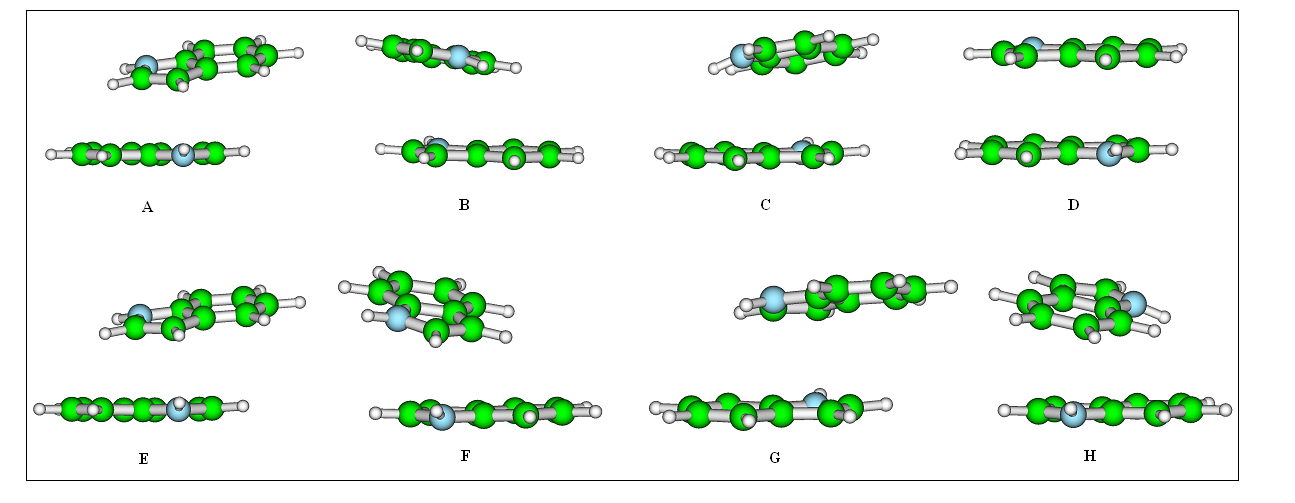
\includegraphics[scale=0.5]{anex/image/Indole-dimers}
		\caption{ Configurations of Indole dimers optimized at the $\omega$B97X-D/6-311++G** level of theory} \label{fig-indoleDI}
	\end{figure}
	
	
	
	\begin{table}[H]
		\caption{ Interaction energies of Indole dimers (kcal/mol) in 8 differents configurations using $\omega$B97X-D/6-311++G**, and compared with SAPT-DFT.}
		\begin{threeparttable}
			\resizebox{17cm}{!}{
				\begin{tabular}{c c c c c c c c c}
					\hline
					& A & B & C & D & E & F & G & H \\ \hline
					\textbf{$\omega$B97X-D/
						6-311++G**} & -9.22 & -9.49 & -10.06 & -9.34 & -9.22 & -6.76 & -9.22 & -10.06 \\ 
					\multicolumn{1}{l}{\textbf{SAPT- DFT(PBE0)
							aug-cc pvtz 
						}} & -7.54 & -7.75 & -8.76 & -8.19 & -7.54 & -5.50 & -7.54 & -8.76 \\ 
						\textbf{LMP2/ 
							aug-cc-pVTZ$^{a}$} &  &  &  & -7.77 &  &  &  &  \\ 
						\textbf{CAM-B3LYP/
							6-31+G*} &  &  & -0.91 &  &  &  &  &  \\ \hline
					\end{tabular}}
					
					\begin{tablenotes}
						\item[a] Ref \cite{fomine2002local}
					\end{tablenotes}
				\end{threeparttable}
				\label{energie-indoleDi}
			\end{table}




\begin{figure}[H]
	\centering
	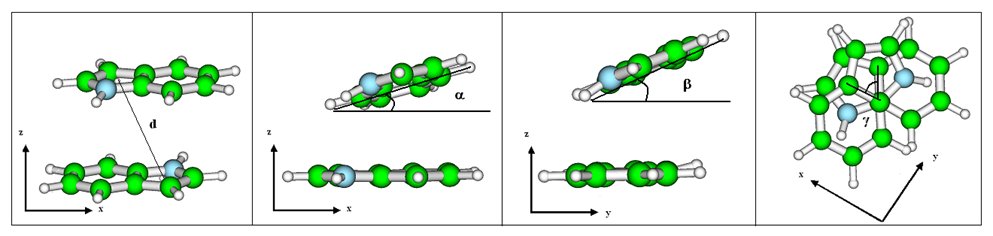
\includegraphics[scale=0.6]{anex/image/Indole-ejes}
	\caption{Structural parameters of Indole dimers}
\end{figure}

	\begin{table}[H]
		\caption{Intermolecular distance between pyrrole rings center of Indole dimers (Å)}
		\begin{center}
			\begin{tabular}{c c c c c c}
				\hline
				\multicolumn{1}{l}{} & \textbf{A=E=G} & \textbf{B} & \textbf{C = H} & \textbf{D} & \textbf{F} \\ \hline
				\textbf{$\omega$B97x-D/
					6-311++G**} & 3.71 & 3.55 &3.44 &4.12 & 4.01 \\
				\textbf{DFT-SAPT(PBE0)/
					aug-cc pvtz} & 3.72 &3.57  &3.46 & 4.13 & 4.04\\ 
				\textbf{CAM-B3LYP/
					6-31+G*} &  &  & 3.57 &  &  \\ 
				\bottomrule
			\end{tabular}
			\label{distance-indoleDi}
		\end{center}
	\end{table}
	
	
	\begin{table}[H]
		\caption{Angle between ring planes of Indole dimers ($^{\circ}$) at the $\omega$B97x-D/6-311++G** level of theory, according to figure }
		\begin{center}
			\begin{tabular}{c c c c c c c}
				\hline
				& \textbf{A = E =G} & \textbf{B} & \textbf{C = H } & \multicolumn{1}{p{4cm}}{\centering \textbf{C (CAM-B3LYP/ \\ 6-31+G*)}} & \textbf{D} & \textbf{F} \\ \hline
				\textbf{$\alpha$
				} & 21.80 & 16.82 & 18.19 & 22.91 & 0.59 & 15.73 \\ 
				\textbf{$\beta$
				} & 26.05 & 6.06 & 15.06 & 23.94 & 2.11 & 22.04 \\ 
				\textbf{$\gamma$
				} & 45.40 & 76.65 & 61.23 & 59.43 & 0.003 & 87.25 \\ \hline
			\end{tabular}
		\end{center}
		\label{indoleDi-parameter}
	\end{table}




	\begin{table}[H]
		\caption{Calculated low wavenumber Raman ad PA infrared spectra of Indole Dimer.}
		\begin{center}
			\begin{threeparttable}
				\begin{tabular}{c c c c c c c c}
					\toprule
					\textbf{Mode} & \textbf{$\omega$ cm$^{-1}$} & \multicolumn{1}{p{3cm}}{\centering \textbf{Intensities} \\ \textbf{($^{a}$) [$^{b}$]}}&  &  & \textbf{Mode} & \textbf{$\omega$ cm$^{-1}$} & \multicolumn{1}{p{3cm}}{\centering \textbf{Intensities} \\ \textbf{($^{a}$) [$^{b}$]}}\\
					\midrule
		$\nu_{1}$	&	29	&	(0.44)	[1.84]& & &	$\nu_{13}$	&	437	&	(35.80)	[0.23]\\
		$\nu_{2}$	&	40	&	(0.57)	[7.68]& & &	$\nu_{14}$	&	444	&	(0.67)	[0.70]\\
		$\nu_{3}$	&	47	&	(0.03)	[5.44]& & &	$\nu_{15}$	&	474	&	(140.28)	[2.59]\\
		$\nu_{4}$	&	73	&(2.63)	[0.58]	& & & 	$\nu_{16}$	&	513	&	(134.92)	[2.75]\\
		$\nu_{5}$	&	89	&	(0.09)	[2.10]& & & 	$\nu_{17}$	&	555	&	(0.30)	[5.40]\\
		$\nu_{6}$	&	129	&	(0.43)	[4.17]&&  & 	$\nu_{18}$	&	556	&	(0.88)	[6.59]\\
		$\nu_{7}$	&	230	&	(18.65)	[1.38]& & &	$\nu_{19}$&	594	&	(0.33)	[0.08]	\\
		$\nu_{8}$	&	234	&	(0.37)	[1.05]& & &	$\nu_{20}$	&	596	&	(0.49)	[0.22]\\
		$\nu_{9}$	&	259	&	(1.03)	[0.13]&  & &	$\nu_{21}$	&	618	&	(4.31)	[1.08]\\
		$\nu_{10}$	&	262	&	(3.19)	[0.06]& & &	$\nu_{22}$	&	623	&	(8.48)	[0.88]\\
		$\nu_{11}$	&	406	&	(1.38)	[0.11]&  & &	$\nu_{23}$	&	626	&	(4.37)	[8.28]\\
		$\nu_{12}$	&	408	&	(5.90)	[0.43]&  & &	$\nu_{24}$	&	627	&	(19.85)	[1.87]\\
		\bottomrule			
				\end{tabular}
				
				\begin{tablenotes}
					\item[a] km/mole
					\item[b] A$^{4}$/AMU
				\end{tablenotes}
			\end{threeparttable}
		\end{center}
		\label{lowfreq-IndoleDi}
	\end{table}


	\begin{table}[H]
		\caption{Calculated Raman and PA infrared spectra of Indole Dimer, 700–2000 cm$^{-1}$}
		\begin{center}
			\begin{threeparttable}
				\begin{tabular}{c c c c c c c c}
					\toprule
					\textbf{Mode} & \textbf{$\omega$ cm$^{-1}$} & \multicolumn{1}{p{3cm}}{\centering \textbf{Intensities} \\ \textbf{($^{a}$) [$^{b}$]}}& &  & \textbf{Mode} & \textbf{$\omega$ cm$^{-1}$} & \multicolumn{1}{p{3cm}}{\centering \textbf{Intensities} \\ \textbf{($^{a}$) [$^{b}$]}}\\
					\midrule
					$\nu_{25}$&	734&	(63.11)	[0.08]	& & &	$\nu_{51}$&	1150&	(0.25)	[0.22]\\
					$\nu_{26}$&	743	&(0.57)	[1.09]& & &	$\nu_{52}$&	1152&	(1.13)	[9.76]\\
					$\nu_{27}$&	769	&(231.13)	[0.35] & & &	$\nu_{53}$&	1179&	(0.75)	[1.87]\\
					$\nu_{28}$&	771	&(4.75)	[0.66] & & & 	$\nu_{54}$&	1179&	(0.82)	[0.40]\\
					$\nu_{29}$&	784&	(9.54)	[0.99] & & &	$\nu_{55}$&	1237&	(4.46)	[2.12]\\
					$\nu_{30}$&	785&	(0.65)	[40.14] & & &	$\nu_{56}$&	1237&	(4.58)	[1.47]\\
					$\nu_{31}$&	794&	(65.87)	[0.48] & & &$\nu_{57}$&	1278&	(10.76)	[8.48]\\
					$\nu_{32}$&	797&	(0.36)	[0.79] & & &	$\nu_{58}$&	1279&	(3.50)	[3.26]\\
					$\nu_{33}$&	872&	(0.75)	[0.22] & & &	$\nu_{59}$&	1318&	(2.92)	[25.37]\\
					$\nu_{34}$&	877&	(1.59)	[0.16] & & &	$\nu_{60}$&	1321&	(16.15)	[7.90]\\
					$\nu_{35}$&	893&	(0.08)	[0.58] & & &	$\nu_{61}$&	1381&	(25.17)	[1.48]\\
					$\nu_{36}$&	894&	(0.22)	[2.32] & & &	$\nu_{62}$&	1382&	(30.25)	[38.1]\\
					$\nu_{37}$&	898&	(1.63)	[1.53] & & &	$\nu_{63}$&	1391&	(6.47)	[13.89]\\
					$\nu_{38}$&	899&	(0.73)	[2.74] & & &	$\nu_{64}$&	1391&	(4.12)	[5.82]\\
					$\nu_{39}$&	921&	(2.94)	[9.77] & & &	$\nu_{65}$&	1469&	(19.27)	[21.23]\\
					$\nu_{40}$&	921&	(7.25)	[0.57] & & &	$\nu_{66}$&	1506&	(4.04)	[3.07]\\
					$\nu_{41}$&	960&	(5.44)	[0.22] & & &	$\nu_{67}$&	1508&	(55.53)	[15.45]\\
					$\nu_{42}$&	964&	(1.32)	[0.45] & & &	$\nu_{68}$&	1540&	(8.42)	[9.06]\\
					$\nu_{43}$&	995&	(0.20)	[0.03] & & &	$\nu_{69}$&	1543&	(0.06)	[3.52]\\
					$\nu_{44}$&	996&	(0.35)	[0.24] & & &	$\nu_{70}$&	1576&	(10.62)	[41.44]\\
					$\nu_{45}$&	1042&	(4.32)	[45.88]	 & &&$\nu_{71}$&	1578&	(6.87)	[103.97]\\
					$\nu_{46}$&	1043&	(9.13)	[1.20] & & &	$\nu_{72}$&	1649&	(0.09)	[7.24]\\
					$\nu_{47}$&	1097&	(2.00)	[21.10] & & &	$\nu_{73}$&	1650&	(0.58)	[7.24]\\
					$\nu_{48}$&	1097&	(2.57)	[3.72] & & &	$\nu_{74}$&	1691&	(0.08)	[7.09]\\
					$\nu_{49}$&	1128&	(12.77)	[5.03] & & &	$\nu_{75}$&	1692&	(3.47)	[21.19]\\
					\bottomrule
				\end{tabular}
				
				\begin{tablenotes}
					\item[a] km/mole
					\item[b] A$^{4}$/AMU
				\end{tablenotes}
			\end{threeparttable}
		\end{center}
		\label{freq-IndoleDi}
	\end{table}
	
		\begin{figure}[H]
			\centering
			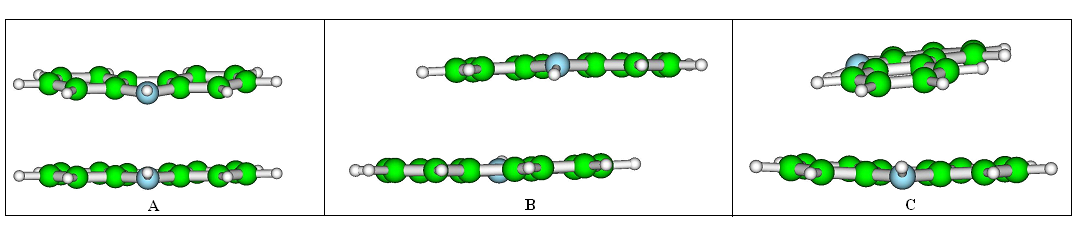
\includegraphics[scale=0.5]{image/Carbazole-dimer}
			\caption{Configurations of Carbazole dimers optimized at the $\omega$B97x-D/6-311++G** level of theory.}  \label{fig-carbazoleDi}
		\end{figure}
		
		
		\begin{table}[H]
			\caption{Interaction energies of Carbazole dimers (kcal/mol) in 3 different configurations using $\omega$B97x-D/6-311++G**.}
			\begin{center}
				\begin{tabular}{c c c c}
					\hline
					& \textbf{A} & \textbf{B} & \textbf{C} \\ \hline
					$\omega$B97x-D/
					6-311++G** & -10.09 & -12.08 & -14.57 \\ \hline
				\end{tabular}
			\end{center}
			\label{energie-carbazoleDi}
		\end{table}
		
		
		\begin{table}[H]
			\caption{Intermolecular distance between pyrrole ring center (Å) and angles ($^{\circ}$) according figure  of  Carbazole dimers using $\omega$B97x-D/6-311++G**.}
			\begin{center}
				\begin{tabular}{c c c c}
					\hline
					& \multicolumn{1}{c}{\textbf{A}} & \multicolumn{1}{c}{\textbf{B}} & \multicolumn{1}{c}{\textbf{C}} \\ \hline
					\textbf{d} & \multicolumn{1}{r}{3.68} & \multicolumn{1}{r}{4.02} & \multicolumn{1}{r}{3.30} \\ 
					\textbf{$\alpha$}& 5.01 & 1.59 & 4.30 \\ 
					\textbf{$\beta$} & 12.60 & 4.17 &6.01 \\ 
					\textbf{$\gamma$} & \multicolumn{1}{c}{} & \multicolumn{1}{c}{} & \multicolumn{1}{c}{76.83} \\ \hline
				\end{tabular}
			\end{center}
			\label{}
		\end{table}
		
		
			\begin{table}[H]
				\caption{Calculated low wavenumber Raman ad PA infrared spectra of Carbazole Dimer.}
				\begin{center}
					\begin{threeparttable}
						\begin{tabular}{c c c c c c c c }
							\toprule
							\textbf{Mode} & \textbf{$\omega$ cm$^{-1}$} & \multicolumn{1}{p{3cm}}{\centering \textbf{Intensities} \\ \textbf{($^{a}$) [$^{b}$]}}& &  &\textbf{Mode} & \textbf{$\omega$ cm$^{-1}$} & \multicolumn{1}{p{3cm}}{\centering \textbf{Intensities} \\ \textbf{($^{a}$) [$^{b}$]}} \\
							\midrule
							$\nu_{1}$&	26&	(0.05)	[4.28]& & &	$\nu_{19}$&	437&	(77.32)	[9.71]\\
							$\nu_{2}$&	31&	(0.03)	[8.66]& & & 	$\nu_{20}$	&438&	(11.67)	[2.22]\\
							$\nu_{3}$&	43&	(0.02)	[8.30]& & &	$\nu_{21}$&	446&	(203.96)	[0.35]\\
							$\nu_{4}$&	65&	(1.32)	[0.40] & & &	$\nu_{22}$&	447&	(30.19)	[0.63]\\
							$\nu_{5}$&	70&	(0.008)	[1.17]& & & 	$\nu_{23}$&	457&	(13.23)	[0.08]\\
							$\nu_{6}$&	95&	(0.51)	[2.21]& & & 	$\nu_{24}$&	458&	(0.01)	[0.37]\\
							$\nu_{7}$&	115&	(2.85)	[0.89]& & &	$\nu_{25}$&	520&	(1.52)	[0.18]\\
							$\nu_{8}$&	153	&(0.12)	[0.08]& & & 	$\nu_{26}$&	521&	(3.61)	[1.57]\\
							$\nu_{9}$&	158&	(0.11)	[0.54]& & &	$\nu_{27}$&	568&	(0.37)	[0.68]\\
							$\nu_{10}$&	168	&(0.04)	[0.85]& & &	$\nu_{28}$&	568&	(0.61)	[12.89]\\
							$\nu_{11}$&	221&	(0.47)	[1.28]& & &$\nu_{29}$&	584&	(0.02)	[0.31]\\
							$\nu_{12}$&	221&	(0.35)	[1.46]& & &	$\nu_{30}$&	585&	(22.52)	[0.20]\\
							$\nu_{13}$&	301&	(0.74)	[4.64]& & &	$\nu_{31}$	&594&	(1.87)	[0.07]\\
							$\nu_{14}$&	305&	0.005	[3.61]& & &	$\nu_{32}$&	596&	(0.01)	[0.03]\\
							$\nu_{15}$&	321&	(0.01)	[0.05]& & &	$\nu_{33}$&	635&	(2.63)	[0.01]\\
							$\nu_{16}$&	325&	(2.83)	[0.06]& & &	$\nu_{34}$&	635&	(4.06)	[0.02]\\
							$\nu_{17}$&	431&	(7.50)	[0.09]& & &	$\nu_{35}$&	678&	(4.03)	[0.48]\\
							$\nu_{18}$&	435&	(5.63)	[17.54]& & &	$\nu_{36}$&	679&	(1.77)	[1.81]\\
							\bottomrule
						\end{tabular}
						
						\begin{tablenotes}
							\item[a] km/mole
							\item[b] A$^{4}$/AMU
						\end{tablenotes}
					\end{threeparttable}
				\end{center}
				\label{low-freqCarbazoleDi}
			\end{table}
			
			
	\begin{table}[H]
		\caption{Calculated Raman and PA infrared spectra of Carbazole Dimer, 700–2000 cm$^{-1}$}
		\begin{center}
			\begin{threeparttable}
				\begin{tabular}{c c c c c c c c}
					\toprule
					\textbf{Mode} & \textbf{$\omega$ cm$^{-1}$} & \multicolumn{1}{p{3cm}}{\centering \textbf{Intensities} \\ \textbf{($^{a}$) [$^{b}$]}}& &  & \textbf{Mode} & \textbf{$\omega$ cm$^{-1}$} & \multicolumn{1}{p{3cm}}{\centering \textbf{Intensities} \\ \textbf{($^{a}$) [$^{b}$]}}\\
					\midrule
					$\nu_{37}$&	750&(241.17)	[0.24]& & & 	$\nu_{73}$&	1179&	(6.29)	[0.40]\\
					$\nu_{38}$&	754	&(0.02)	[0.26]& & & 	$\nu_{74}$&	1179&	(3.39)	[7.54]\\
					$\nu_{39}$&	762&	(4.39)	[1.11]& & & 	$\nu_{75}$&	1187&	(0.41)	[3.90]\\
					$\nu_{40}$&	765	&(4.98)	[2.93]& & &	$\nu_{76}$&	1187&	(1.02)	[0.43]\\
					$\nu_{41}$&	767	&(15.18)	[0.45]& & & 	$\nu_{77}$&	1244&	(9.48)	[17.02]\\
					$\nu_{42}$&	767	&(0.32)	[44.78]& & & 	$\nu_{78}$&	1245&	(2.29)	[31.39]\\
					$\nu_{43}$&	781	&(0.07)	[1.06]& & & 	$\nu_{79}$&	1254&	(0.38) [3.53]\\
					$\nu_{44}$&	782	&(108.04)	[0.10]& & & 	$\nu_{80}$&	1254&	(1.17)	[1.38]\\
					$\nu_{45}$&	796	&(1.02)	[0.73]& & & 	$\nu_{81}$&	1277&	(44.62)	[0.76]\\
					$\nu_{46}$&	802	&(0.62)	[1.65]& & & 	$\nu_{82}$&	1278&	(73.55)	[13.45]\\
					$\nu_{47}$&	869	&(3.99)	[0.41]& & & 	$\nu_{83}$&	1328&	(0.17)	[89.36]\\
					$\nu_{48}$&	870	&(3.84)	[0.19]& & & 	$\nu_{84}$&	1329&	(2.37)	[30.66]\\
					$\nu_{49}$&	873	&(1.59)	[0.04]& & & 	$\nu_{85}$&	1347&	(1.42)	[44.81]\\
					$\nu_{50}$&	873	&(1.99)	[1.14]& & & 	$\nu_{86}$&	1348&	(0.02)	[169.47]\\
					$\nu_{51}$&	877	&(4.42)	[0.36]& &  &	$\nu_{87}$&	1365&	(4.44)	[0.08]\\
					$\nu_{52}$&	881	&(2.57)	[0.67]& & & 	$\nu_{88}$&	1365&	(57.98)	[2.21]\\
					$\nu_{53}$&	902	&(2.28)	[3.33]& & & 	$\nu_{89}$&	1375&	(9.18)	[23.33]\\
					$\nu_{54}$&	902	&(0.009)	[30.50]& & & 	$\nu_{80}$&	1377&	(11.37)	[7.82]\\
					$\nu_{55}$&	958	&(0.14)	[0.30]	& & & $\nu_{81}$&	1438&	(9.27)	[5.06]\\
					$\nu_{56}$&	958	&(6.99)	[0.08]& & & 	$\nu_{82}$&	1439&	(5.14)	[0.35]\\
					$\nu_{57}$&	962	&(0.83)	[0.08]& & & 	$\nu_{83}$&	1501&	(12.98)	[10.05]\\
					$\nu_{58}$&	963	&(1.56)	[0.28]& &  &	$\nu_{84}$&	1503&	(31.33)	[30.01]\\
					$\nu_{59}$&	994	&(0.03)	[0.15]& &  &	$\nu_{85}$&	1509&	(34.71)	[0.57]\\
					$\nu_{60}$&	996	&(1.08)	[0.01]& &  &	$\nu_{86}$&	1509&	(43.83)	[0.85]\\
					$\nu_{61}$&	996	&(0.59)	[0.26]& & & 	$\nu_{87}$&	1538&	(0.64)	[27.23]\\
					$\nu_{62}$&	997	&(0.00)	[0.09]& & & 	$\nu_{88}$&	1539&	(0.95)	[39.33]\\
					$\nu_{63}$&	1028&	(3.64)	[0.93]& & & 	$\nu_{89}$&	1547&	(33.20)	[2.87]\\
					$\nu_{64}$&	1028&	(5.18)	[2.21]& & & 	$\nu_{90}$&	1549&	(43.02)	[4.01]\\
					$\nu_{65}$&	1048&	(0.00)	[88.19]& &  &	$\nu_{91}$&	1649	&(1.39)	[57.62]\\
					$\nu_{66}$&	1049&	(2.21)	[5.40]	& &  &$\nu_{92}$&	1649&	(0.02)	[19.29]\\
					$\nu_{67}$&	1053&	(4.46)	[0.42]& & & 	$\nu_{93}$&	1657&	(2.86)	[2.36]\\
					$\nu_{68}$&	1054&	(7.89)	[3.51]& & & 	$\nu_{94}$&	1658&	(5.23)	[20.96]\\
					$\nu_{69}$&	1140&	(5.75)	[1.19]& & & 	$\nu_{95}$&	1681&	(29.56)	[17.35]\\
					$\nu_{70}$&	1140&	(3.15)	[17.48]& & & 	$\nu_{96}$&	1682&	(26.68)	[0.31]\\
					$\nu_{71}$&	1151&	(2.91)	[0.10]	& & & $\nu_{97}$&	1707&	(9.47)	[121.78]\\
					$\nu_{72}$&	1151&	(5.66)	[2.23]& & & 	$\nu_{98}$&	1707&	(1.58)	[124.42]\\
					\bottomrule
				\end{tabular}
				
				\begin{tablenotes}
					\item[a] km/mole
					\item[b] A$^{4}$/AMU
				\end{tablenotes}
			\end{threeparttable}
		\end{center}
		\label{freqCarbazoleDi}
	\end{table}
	
	
	\begin{figure}[H]
		\centering
		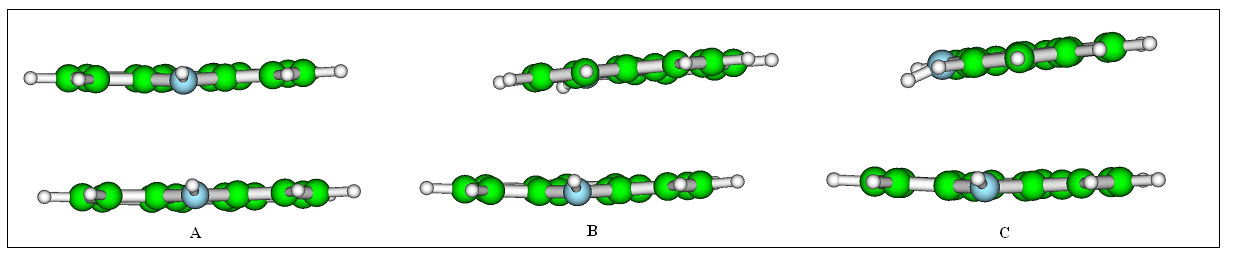
\includegraphics[scale=0.5]{image/45-iminopphenanthrene}
		\caption{Configurations of 4,5-iminophenanthrene dimers optimized at the $\omega$B97X-D/6-311++G** level of theory.}  \label{fig-45-iminoDi}
	\end{figure}
	
	
	\begin{table}[H]
		\caption{Interaction energies of 4,5-iminophenanthrene dimers (kcal/mol) using $\omega$B97X-D/6-311++G**.}
		\begin{center}
			\begin{tabular}{c c c c}
				\hline
				& \textbf{A} & \textbf{B} & \textbf{C} \\ \hline
				\textbf{$\omega$B97x-D/
					6-311++G**} & -12.78 & -15.13 & -14.78 \\ \hline
			\end{tabular}
		\end{center}
		\label{}
	\end{table}
	
	\begin{table}[H]
		\caption{Intermolecular distance between pyrrole ring center (Å) and angles ($^{\circ}$) according figure  of  4,5-iminophenanthrene dimers using $\omega$B97x-D/6-311++G**.}
		\begin{center}
			\begin{tabular}{c c c c}
				\hline
				& \multicolumn{1}{c}{\textbf{A}} & \multicolumn{1}{c}{\textbf{B}} & \multicolumn{1}{c}{\textbf{C}} \\ \hline
				\textbf{d} & \multicolumn{1}{r}{3.66} & \multicolumn{1}{r}{3.59} & \multicolumn{1}{r}{3.66} \\ 
				\textbf{$\alpha$}& 2.60 &10.25 & 5.76 \\ 
				\textbf{$\beta$} & 4.84 & 8.42 & 8.65\\ 
				\textbf{$\gamma$} & &  &73.64 \\ \hline
			\end{tabular}
		\end{center}
		\label{}
	\end{table}
	
	
	\begin{table}[H]
		\caption{Calculated low wavenumber Raman ad PA infrared spectra of 4,5-iminophenanthrene Dimer.}
		\begin{center}
				\begin{tabular}{c c c c c c c c}
					\toprule
					\textbf{Mode} & \textbf{$\omega$ cm$^{-1}$} & \multicolumn{1}{p{3cm}}{\centering \textbf{Intensities} \\ \textbf{($^{a}$) [$^{b}$]}}&  & &\textbf{Mode} & \textbf{$\omega$ cm$^{-1}$} & \multicolumn{1}{p{3cm}}{\centering \textbf{Intensities} \\ \textbf{($^{a}$) [$^{b}$]}} \\
					\midrule			
$\nu_{1}$&	19&	(0.05)	[1.55]&  & &	$\nu_{11}$&	220	&(0.19)	[0.07]\\
$\nu_{2}$&	31&	(0.86)	[10.03]	& & &$\nu_{12}$&	224	&(17.06)	[0.10]\\
$\nu_{3}$&	38&	(0.06)	[8.52]& & &	$\nu_{13}$&	313	&(0.15)	[0.93]\\
$\nu_{4}$&	61&	(0.60)	[0.89]&  & &	$\nu_{14}$&	314&	(0.22)	[0.06]\\
$\nu_{5}$&	75&	(1.88)	(0.84)& & &	$\nu_{15}$&	322&	(2.12)	[2.57]\\
$\nu_{6}$&	92&	(1.31)	[5.95]& & &	$\nu_{16}$&	326&	(0.97)	[1.26]\\
$\nu_{7}$&	114&	(6.79)	[0.33]& & &	$\nu_{17}$&	352&	(3.60)	[0.45]\\
$\nu_{8}$&	128	&(0.52)	[3.59]& & &	$\nu_{18}$&	353&	(3.52)	[0.28]\\
$\nu_{9}$&	202&	(0.71)	[0.62]& & &	$\nu_{19}$&	376&	(192.54)	[11.49]\\
$\nu_{10}$&	205&	(0.10)	[1.07]& & &	$\nu_{20}$&	416&	(144.55)	[7.09]\\
	\bottomrule
	\end{tabular}
\end{center}
\end{table}



	\begin{table}[H]
		\begin{center}
			\begin{threeparttable}
            	\begin{tabular}{c c c c c c c c}
            		\toprule
            		\textbf{Mode} & \textbf{$\omega$ cm$^{-1}$} & \multicolumn{1}{p{3cm}}{\centering \textbf{Intensities} \\ \textbf{($^{a}$) [$^{b}$]}}&  & &\textbf{Mode} & \textbf{$\omega$ cm$^{-1}$} & \multicolumn{1}{p{3cm}}{\centering \textbf{Intensities} \\ \textbf{($^{a}$) [$^{b}$]}} \\
            		\midrule	
  $\nu_{21}$&	446&	(0.18)	[2.38]& & &	$\nu_{32}$&	581&	(0.03)	[1.82]\\
  $\nu_{22}$&	447&	(0.12)	[1.83]& & &	$\nu_{33}$&	586&	(0.03)	[0.26]\\
  $\nu_{23}$&	458&	(0.52)	[20.91]& & &	$\nu_{34}$&	586&	(0.02)	[0.17]\\
  $\nu_{24}$&	458&	(5.85)	[10.36]& & &	$\nu_{35}$&	613&	(1.60)	[0.18]\\
  $\nu_{25}$&	492&	(2.23)	[2.10]& & &	$\nu_{36}$&	616&	(0.48)	[0.49]\\
  $\nu_{26}$&	492&	(2.63)	[2.11]& & &	$\nu_{37}$&	621&	(6.47)	[5.71]\\
  $\nu_{27}$&	508&	(5.40)	[0.10]& & &	$\nu_{38}$&	622&	(1.86)	[44.52]\\
  $\nu_{28}$&	509&	(0.38)	[0.53]& & &	$\nu_{39}$&	664&	(0.69)	[0.15]\\
  $\nu_{29}$&	549&	(0.10)	[1.74]& & &	$\nu_{40}$&	666&	(0.17)	[0.11]\\
  $\nu_{30}$&	550&	(0.07)	[1.54]& & &	$\nu_{41}$&	698&	(2.18)	[8.38]\\
  $\nu_{31}$&	581&	(0.02)	[1.66]& & &	$\nu_{42}$&	699&	(1.51)	[22.84]\\
  \bottomrule
   \end{tabular}
         		
         		\begin{tablenotes}
         			\item[a] km/mole
         			\item[b] A$^{4}$/AMU
         		\end{tablenotes}
         	\end{threeparttable}
         \end{center}
         \label{lowfreq-45-iminoDi}
        \end{table}   		




  \begin{table}[H]
  	\caption{Calculated Raman and PA infrared spectra of 4,5-iminophenantrene Dimer, 700–2000 cm$^{-1}$}
  	\begin{center}
  			\begin{tabular}{c c c c c c c c}
  				\toprule
  				\textbf{Mode} & \textbf{$\omega$ cm$^{-1}$} & \multicolumn{1}{p{3cm}}{\centering \textbf{Intensities} \\ \textbf{($^{a}$) [$^{b}$]}}& &  & \textbf{Mode} & \textbf{$\omega$ cm$^{-1}$} & \multicolumn{1}{p{3cm}}{\centering \textbf{Intensities} \\ \textbf{($^{a}$) [$^{b}$]}}\\
  				\hline
  				$\nu_{43}$&	711&	0,27	0,07& & &	$\nu_{62}$&	1204&	3,46	1\\
  				$\nu_{44}$&	711	&0,04	0,28& & &	$\nu_{63}$&	1214	&5,39	10,15\\
  				$\nu_{45}$&	739&	128,75	0,53& & &	$\nu_{64}$&	1214&	7,53	7,26\\
  				$\nu_{46}$&	740&	8,29	0,91& & &	$\nu_{65}$&	1246&	6,75	15,67\\
  				$\nu_{47}$&	772&	28,65	0,63& & & 	$\nu_{66}$&	1246&	0,32	64,88\\
  				$\nu_{48}$&	775&	28,81	0,23& & &	$\nu_{67}$&	1250&	0,52	0,41\\
  				$\nu_{49}$&	776&	3,79	1,89& & &	$\nu_{68}$&	1251&	0,15	2,34\\
  				$\nu_{50}$&	778&	8,6	0,79& & &	$\nu_{69}$&	1264	&4,78	2,77\\
  				$\nu_{51}$&	822&	0,06	0,43& & &	$\nu_{70}$&	1265&	11,08	2.3\\
  				$\nu_{52}$&	823&	0,01	0,68& & &	$\nu_{71}$&	1283&	1,07	31,8\\
  				$\nu_{53}$&	831&	1,96	1,33& & &	$\nu_{72}$&	1284&	2,77	8,74\\
  				$\nu_{54}$&	834&	1,06	2,16& & &	$\nu_{73}$&	1363&	7,13	3,08\\
  				$\nu_{55}$&	843&	43,96	2,87& & &	$\nu_{74}$&	1364&	52,26	1,89\\
  				$\nu_{56}$&	843&	8,2	7,55& & & 	$\nu_{75}$&	1366	&2,83	73,43\\
  				$\nu_{57}$&	846&	137,09	0,3& & &	$\nu_{56}$&	1367&	29,2	34,08\\
  				$\nu_{58}$&	847&	2,55	1,88& & &	$\nu_{57}$&	1395&	0,34	14,67\\
  				$\nu_{59}$&	894&	1,29	0,51& & &	$\nu_{58}$&	1395&	0,29	16,55\\
  				$\nu_{60}$&	896&	1,13	0,46& & & 	$\nu_{59}$&	1433&	28.00	0,77\\
  				$\nu_{61}$&	903&	6,39	0,17& & & 	$\nu_{60}$&	1434&	46,35	0,22\\
  				$\nu_{62}$&	904&	1,81	0,36& & & 	$\nu_{61}$&	1447&	4,55	36,99\\
  				$\nu_{63}$&	983&	0,7	0,2& & &	$\nu_{62}$&	1447	&1,53	36,46\\
  				$\nu_{64}$&	985&	0,12	0,11& & &	$\nu_{63}$&	1485&	9,86	0,84\\
  				$\nu_{65}$&	986&	0,88	0,09& & & 	$\nu_{64}$&	1485&	5,65	0,84\\
  				\bottomrule
  			\end{tabular}
  		\end{center}
  	\end{table}
  	
  	
  	
  	
  	
  	
  	\begin{table}[H]
  		\begin{center}
  			\begin{threeparttable}
  				\begin{tabular}{c c c c c c c c}
  					\toprule
  					\textbf{Mode} & \textbf{$\omega$ cm$^{-1}$} & \multicolumn{1}{p{3cm}}{\centering \textbf{Intensities} \\ \textbf{($^{a}$) [$^{b}$]}}& &  & \textbf{Mode} & \textbf{$\omega$ cm$^{-1}$} & \multicolumn{1}{p{3cm}}{\centering \textbf{Intensities} \\ \textbf{($^{a}$) [$^{b}$]}}\\
  					\hline  				
  				$\nu_{66}$&	987&	2,61	0,07& & & 	$\nu_{65}$&	1491&	8,97	45,65\\
  				$\nu_{67}$&	1001&	0,11	0,79& &  &	$\nu_{66}$&	1492&	26,35	11,69\\
  				$\nu_{68}$&	1001&	0,45	2,85& & &	$\nu_{67}$&	1532&	1,09	327,53\\
  				$\nu_{69}$&	1030&	0,26	0,81& & & 	$\nu_{68}$&	1533&	0,87	141,8\\
  				$\nu_{70}$&	1030&	0,45	1,22& & & 	$\nu_{69}$&	1555&	0,62	0,79\\
  				$\nu_{71}$&	1050&	0,05	5,17& & &	$\nu_{70}$&	1556&	1,31	0,22\\
  				$\nu_{72}$&	1051&	0,59	0,12& & & 	$\nu_{71}$&	1567&	6,88	8,72\\
  				$\nu_{73}$&	1060&	0,83	35,07& & & 	$\nu_{72}$&	1568&	27,68	3,99\\
  				$\nu_{74}$&	1060&	0,56	24,98& & & 	$\nu_{73}$&	1670&	37,28	0,89\\
  				$\nu_{75}$&	1076&	0,27	2,12& &  &	$\nu_{74}$&	1672&	110,36	2,52\\
  				$\nu_{56}$&	1077&	0,64	2,08& & &	$\nu_{75}$&	1674&	0,85	11,45\\
  				$\nu_{57}$&	1104&	15,85	5,11& & &	$\nu_{56}$&	1675&	14,04	13,97\\
  				$\nu_{58}$&	1105&	57,86	6,45& & &	$\nu_{57}$&	1708&	3,04	66,33\\
  				$\nu_{59}$&	1165&	0,75	2,8	& & &$\nu_{58}$&	1709&	7	81,57\\
  				$\nu_{60}$&	1165&	0,19	6,46& & & 	$\nu_{59}$&	1738&	0,23	4,52\\
  				$\nu_{61}$&	1202&	0,6	0,4	& & & $\nu_{60}$&	1740	&0,6	5,4\\
  			\bottomrule
  			\end{tabular}
  			
  			\begin{tablenotes}
  				\item[a] km/mole
  				\item[b] A$^{4}$/AMU
  			\end{tablenotes}
  		\end{threeparttable}
  	\end{center}
  	\label{freq-45-iminoDi}
  \end{table}



\begin{figure}[H]
	\centering
	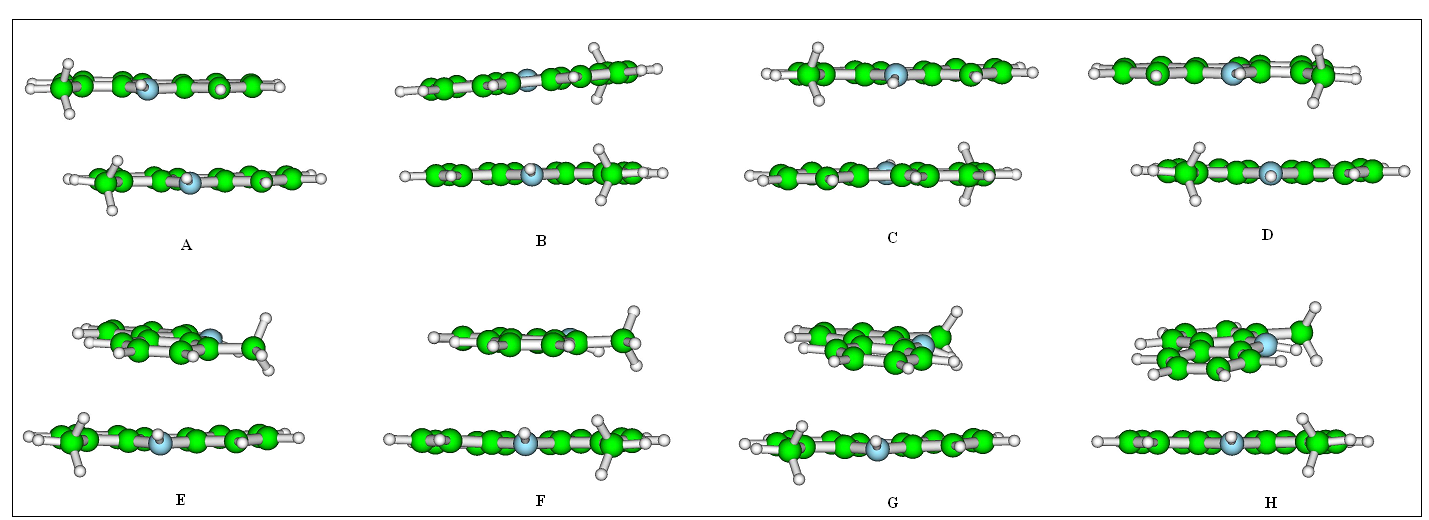
\includegraphics[scale=0.42]{image/1-methylcarbazole}
	\caption{Configurations of 1-methylcarbazole dimers optimized at the $\omega$B97X-D/6-311++G** level of theory.}
\end{figure}



\begin{table}[H]
	\caption{Interaction energies of 1-methylcarbazole dimers (kcal/mol) using $\omega$B97X-D/6-311++G**.}
	\begin{center}
		\begin{tabular}{c c c c c c c c c}
			\hline
			& A & B & C & D & E & F & G & H \\ \hline
			\textbf{$\omega$B97X-D/
				6-311++G**} & -11.81 & -15.04 & -15.03 & -12.27 & -15.62 & -16.10 & -15.91 & -14.81 \\ \hline
		\end{tabular}
	\end{center}
	\label{}
\end{table}

	\begin{table}[H]
		\caption{Intermolecular distance between pyrrole ring center (Å) and plane angles ($^{\circ}$)  of 1-methylcarbazole dimers with the $\omega$B97x-D/6-311++G**.}
		\begin{center}
			\begin{tabular}{ c c c c c c c c c}
				\hline
				\multicolumn{1}{l}{} & \textbf{A} & \textbf{B} & \textbf{C} & \textbf{D} & \textbf{E} & \textbf{F} & \textbf{G} & \textbf{H} \\ \hline
				\textbf{d
				} & 3.83 & 3.78 & 3.76 & 3.86 & 3.35 & 3.36 & 3.34 & 3.46 \\ 
				\textbf{$\alpha$
				} & 6.21 & 5.65 & 3.65 & 1.58 & 5.79 & 1.62 & 18.04 & 8.37 \\ 
				\textbf{$\beta$
				} & 6.28 & 4.10 & 5.94 & 5.98 & \multicolumn{1}{r}{10.34} & 10.32 & 6.35 & 16.92 \\ 
				\textbf{$\gamma$
				} &  &  &  &  & 136.11 & 139.65 & 135.39 & 121.90 \\ \hline
			\end{tabular}
		\end{center}
		\label{}
	\end{table}


	\begin{table}[H]
		\caption{Calculated low wavenumber Raman ad PA infrared spectra of 1-methylcarbazole Dimer.}
		\begin{center}
		\begin{threeparttable}
			\begin{tabular}{c c c c c c c c}
				\toprule
				\textbf{Mode} & \textbf{$\omega$ cm$^{-1}$} & \multicolumn{1}{p{3cm}}{\centering \textbf{Intensities} \\ \textbf{($^{a}$)}}&  & &\textbf{Mode} & \textbf{$\omega$ cm$^{-1}$} & \multicolumn{1}{p{3cm}}{\centering \textbf{Intensities} \\ \textbf{($^{a}$)}} \\
				\midrule		
$\nu_{1}$&	28&	(0.13)& & &	$\nu_{22}$& 332& (3.67) \\
$\nu_{2}$&	33&	(0.02)& & &	$\nu_{23}$& 440 &(9.09)\\
$\nu_{3}$&	51&	(0.00)& &	&$\nu_{24}$& 442 &(0.40)\\
$\nu_{4}$& 74 &(0.23)	& & &		$\nu_{25}$& 448& (0.39)\\
$\nu_{5}$&	76 &(0.01)	& & &	$\nu_{26}$& 449& (1.55)\\
$\nu_{6}$&	103& (3.40)& & &		$\nu_{27}$& 510 &(42.79)\\
$\nu_{7}$&	108 &(0.00)	& & &	$\nu_{28}$& 513 &(3.08)\\
$\nu_{8}$&	125& (0.08)	& & &	$\nu_{29}$&  522 &(23.58)\\
$\nu_{9}$&	136& (0.21)& & &		$\nu_{30}$&  523 &(11.52)\\
$\nu_{10}$&	144& (0.27)&  &	&	$\nu_{31}$&  532 &(30.72)\\
$\nu_{11}$&	149& (0.09)	&& &	$\nu_{32}$&  535& (156.32)\\
$\nu_{12}$&	160& (1.74)& & &		$\nu_{33}$&  571 &(30.52)\\
$\nu_{13}$&	190& (0.49)	 & & &	$\nu_{34}$&  572 &(0.27)\\
$\nu_{14}$&	191& (0.19)&&&		$\nu_{35}$&  591 &(21.30)\\
$\nu_{15}$&	234& (0.01)	& & &	$\nu_{36}$&  591 &(0.92)\\
$\nu_{16}$&	235& (1.82)& & &		$\nu_{37}$&  595 &(4.02)\\
$\nu_{17}$&	298& (0.29)	& & &	$\nu_{38}$&  597 &(0.22)\\
$\nu_{18}$&	303& (0.07)	& & &	$\nu_{39}$&  598 &(4.52)\\
$\nu_{19}$&	306& (0.16)& & &		$\nu_{40}$&  598 &(1.61)\\
$\nu_{20}$&	311& (0.00)& & &		$\nu_{41}$&  660 &(4.41)\\
$\nu_{21}$&	328& (0.34)	& & &	$\nu_{42}$&  660 &(5.78)\\
	\bottomrule
\end{tabular}

\begin{tablenotes}
	\item[a] km/mole
\end{tablenotes}
\end{threeparttable}
\end{center}
\label{lowfreq-1-methylcarbazoleDi}
\end{table}				
				
	
\begin{table}[H]
	\caption{Raman ad PA infrared spectra of 1-methylcarbazole Dimer, 700- 200 cm$^{-1}$.}
	\begin{center}
		\begin{threeparttable}
			\begin{tabular}{c c c c c c c c}
				\toprule
				\textbf{Mode} & \textbf{$\omega$ cm$^{-1}$} & \multicolumn{1}{p{3cm}}{\centering \textbf{Intensities} \\ \textbf{($^{a}$)}}&  & &\textbf{Mode} & \textbf{$\omega$ cm$^{-1}$} & \multicolumn{1}{p{3cm}}{\centering \textbf{Intensities} \\ \textbf{($^{a}$)}} \\
				\midrule		
	$\nu_{43}$&	725	&(1.53)& & &	$\nu_{83}$&	1194&	(0.30)\\
	$\nu_{44}$&	725	&(0.02)& & &	$\nu_{84}$&	1194	&(0.82)\\
	$\nu_{45}$&	755	&(119.18)& & &	$\nu_{85}$&	1251&	(5.99)\\
	$\nu_{46}$&	759	&(3.30)	& & &$\nu_{86}$&	1251	&(0.03)\\
	$\nu_{47}$&	771	&(72.00)& & &	$\nu_{87}$&	1273&	(33.85)\\
	$\nu_{48}$&	774	&(0.21)& & &	$\nu_{88}$&	1275&	(57.37)\\
	$\nu_{49}$&	778	&(111.76)& & &	$\nu_{89}$&	1284	&(0.07)\\
	$\nu_{50}$&	778	&(0.25)	& & &$\nu_{90}$&	1284&	(0.17)\\
	$\nu_{51}$&	814	&(0.01)& & &	$\nu_{91}$&	1321&	(3.08)\\
	$\nu_{52}$&	815	&(8.52)& & &	$\nu_{92}$&	1322&	(5.15)\\
	$\nu_{53}$&	863	&(0.19)& & &	$\nu_{93}$&	1350&	(0.99)\\
	$\nu_{54}$&	864	&(4.19)& & &	$\nu_{94}$&	1351&	(11.68)\\
	$\nu_{55}$&	873	&(0.57)& & &	$\nu_{95}$&	1361&	(38.49)\\
	$\nu_{56}$&	873	&(4.46)& & &	$\nu_{96}$&	1361&	(56.34)\\
	$\nu_{57}$&	883	&(1.44)& & &	$\nu_{97}$&	1376&	(2.20)\\
	$\nu_{58}$&	884	&(4.35)& & &	$\nu_{98}$&	1377&	(17.18)\\
	$\nu_{59}$&	920	&(0.63)& & &	$\nu_{99}$&	1420&	(14.61)\\
	$\nu_{60}$&	921	&(0.00)& & &	$\nu_{100}$&	1421&	(4.72)\\
	$\nu_{61}$&	928	&(1.70)& & &	$\nu_{101}$&	1441&	(0.39)\\
	$\nu_{62}$&	930	&(1.94)& & &	$\nu_{102}$&	1442&	(16.31)\\
	$\nu_{63}$&	959	&(0.52)	& & &$\nu_{103}$&	1466&	(3.15)\\
	$\nu_{64}$&	960	&(3.76)& & &	$\nu_{104}$&	1470&	(37.22)\\
	$\nu_{65}$&	984	&(1.72)& & &	$\nu_{105}$&	1485&	(18.25)\\
	$\nu_{66}$&	984	&(0.00)& & &	$\nu_{106}$&	1493&	(1.58)\\
	$\nu_{67}$&	994	&(0.66)& & &	$\nu_{107}$&	1505&	(8.23)\\
	$\nu_{68}$&	996	&(0.10)& & &	$\nu_{108}$&	1505&	(37.77)\\
	$\nu_{69}$&	1014&	(1.61)& & &	$\nu_{109}$&	1512&	(19.90)\\
	$\nu_{70}$&	1015&	(2.10)& & &	$\nu_{110}$&	1513&	(30.90)\\
	$\nu_{71}$&	1051&	(1.31)& & &	$\nu_{111}$&	1542&	(10.13)\\
	$\nu_{72}$&	1051&	(8.90)& & &	$\nu_{112}$&	1543&	(4.43)\\
	$\nu_{73}$&	1066&	(0.64)& & &	$\nu_{113}$&	1556&	(25.32)\\
	$\nu_{74}$&	1066&	(6.92)& & &	$\nu_{114}$&	1557&	(30.94)\\
	$\nu_{75}$&	1094&	(16.80)& & &	$\nu_{115}$&	1654&	(0.41)\\
	$\nu_{76}$&	1095&	(1.56)& & &	$\nu_{116}$&	1655&	(1.90)\\
	$\nu_{77}$&	1121&	(0.00)& & &	$\nu_{117}$&	1667&	(2.17)\\
	$\nu_{78}$&	1121&	(3.83)& & &	$\nu_{118}$&	1668&	(27.38)\\
	$\nu_{79}$&	1153&	(1.39)& & &	$\nu_{119}$&	1681&	(6.50)\\
	$\nu_{80}$&	1154&	(13.29)& & &	$\nu_{120}$&	1681&	(16.08)\\
	$\nu_{81}$&	1184&	(0.01)& & &	$\nu_{121}$&	1704&	(15.67)\\
	$\nu_{82}$&	1184&	(3.93)& & &	$\nu_{122}$&	1704&	(0.36)\\
	\bottomrule
\end{tabular}

\begin{tablenotes}
	\item[a] km/mole
\end{tablenotes}
\end{threeparttable}
\end{center}
\label{freq-1-methylcarbazoleDi}
\end{table}		
	
	
	\begin{figure}[H]
		\centering
		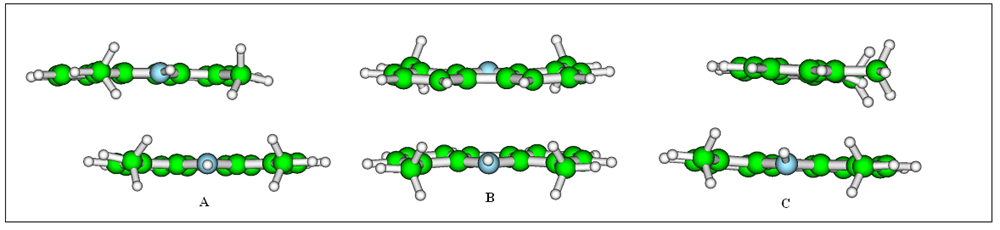
\includegraphics[scale=0.9]{image/18-N}
		\caption{Configurations of 1,8-dimethylcarbazole dimers optimized at the $\omega$B97X-D/6-311++G** level of theory.}
	\end{figure}
	
	\begin{table}[H]
		\caption{Interaction energies of 1,8-dimethylcarbazole dimers (kcal/mol) using $\omega$B97X-D/6-311++G**.}
		\begin{center}
			\begin{tabular}{c c c c}
				\hline
				& \textbf{A} & \textbf{B} & \textbf{C} \\ \hline
				\textbf{$\omega$B97x-D/
					6-311++G**} & -12.83 & -18.72 & -17.72  \\ \hline
			\end{tabular}
		\end{center}
		\label{}
	\end{table}	
	
	
	\begin{table}[H]
		\caption{Intermolecular distance between pyrrole ring center (Å) and angles ($^{\circ}$) according figure  of  1,8-dimethylcarbazole dimers using $\omega$B97x-D/6-311++G**.}
		\begin{center}
			\begin{tabular}{c c c c}
				\hline
				& \multicolumn{1}{c}{\textbf{A}} & \multicolumn{1}{c}{\textbf{B}} & \multicolumn{1}{c}{\textbf{C}} \\ \hline
				\textbf{d} & \multicolumn{1}{r}{} & \multicolumn{1}{r}{} & \multicolumn{1}{r}{} \\ 
				\textbf{$\alpha$}&  & &  \\ 
				\textbf{$\beta$} & &  & \\ 
				\textbf{$\gamma$} & &  & \\ \hline
			\end{tabular}
		\end{center}
		\label{}
	\end{table}		
	
	
\begin{table}[H]
	\caption{Calculated low wavenumber Raman ad PA infrared spectra of 1,8-dimethylcarbazole Dimer.}
	\begin{center}
			\begin{tabular}{c c c c c c c c}
				\toprule
				\textbf{Mode} & \textbf{$\omega$ cm$^{-1}$} & \multicolumn{1}{p{3cm}}{\centering \textbf{Intensities} \\ \textbf{($^{a}$)}}&  & &\textbf{Mode} & \textbf{$\omega$ cm$^{-1}$} & \multicolumn{1}{p{3cm}}{\centering \textbf{Intensities} \\ \textbf{($^{a}$)}} \\
				\midrule			
	$\nu_{1}$&	31&	(0.12)	& & &$\nu_{11}$&	160	&(0.00)\\
	$\nu_{2}$&	34&	(0.00)& & & 	$\nu_{12}$&	160	&(1.48)\\
	$\nu_{3}$&	54&	(0.00)& & & $\nu_{13}$&	180	&(6.56)	\\
	$\nu_{4}$&	73&	(0.00)& & & $\nu_{14}$&	198	&(0.00)	\\
	$\nu_{5}$&	84&	(1.31)& & & 	$\nu_{15}$&	202	&(0.00)\\
	$\nu_{6}$&	103&	(0.00)& & &	$\nu_{16}$&	214	&(0.90)\\
	$\nu_{7}$&	105	&(4.93)& && $\nu_{17}$&	229	&(0.00)	\\
	$\nu_{8}$&	117&	(0.00)& & &$\nu_{18}$	&245&	(4.36)	\\
	$\nu_{9}$&	123	&(0.00)& & &$\nu_{19}$&	250	&(0.02)	\\
	$\nu_{10}$&	125	&(0.00)& && $\nu_{20}$	&268&	(0.00)	\\	
		\bottomrule
	\end{tabular}
\end{center}
\end{table}
	
		
		\begin{table}[H]
			\begin{center}
				\begin{threeparttable}
				\begin{tabular}{c c c c c c c c}
					\toprule
					\textbf{Mode} & \textbf{$\omega$ cm$^{-1}$} & \multicolumn{1}{p{3cm}}{\centering \textbf{Intensities} \\ \textbf{($^{a}$)}}&  & &\textbf{Mode} & \textbf{$\omega$ cm$^{-1}$} & \multicolumn{1}{p{3cm}}{\centering \textbf{Intensities} \\ \textbf{($^{a}$)}} \\
					\midrule		
		$\nu_{20}$ & 280 & (0.00) & & & $\nu_{34}$ & 514 & (0.00) \\ 
		$\nu_{21}$ & 282 & (0.13) && &  $\nu_{35}$ & 515 & (9.44) \\ 
		$\nu_{22}$ & 301 & (0.19) &&& $\nu_{36}$ & 538 & (0.12) \\ 
		$\nu_{23}$ & 306 & (0.00) &&& $\nu_{37}$ & 541 & (0.00) \\ 
		$\nu_{24}$ & 314 & (10.50) &&& $\nu_{38}$ & 567 & (0.00) \\ 
		$\nu_{25}$ & 317 & (0.00) &&& $\nu_{39}$ & 567 & (0.98) \\ 
		$\nu_{26}$ & 329 & (5.77) &&& $\nu_{40}$ & 588 & (0.00) \\ 
		$\nu_{27}$ & 338 & (0.00) &&& $\nu_{41}$ & 589 & (15.27) \\ 
		$\nu_{28}$& 385 & (212.09)&& & $\nu_{42}$ & 591 & (0.00) \\ 
		$\nu_{29}$ & 390 & (0.00) &&& $\nu_{43}$ & 591 & (9.91) \\ 
		$\nu_{30}$ & 476 & (3.47) & &&$\nu_{44}$ & 597 & (0.00) \\ 
		$\nu_{31}$ & 476 & (0.00) & &&$\nu_{45}$ & 597 & (1.32) \\ 
		$\nu_{32}$ & 491 & (0.00) &&& $\nu_{46}$ & 603 & (0.00) \\ 
		$\nu_{33}$ & 492 & (0.00) &&& $\nu_{47}$ & 603 & (1.69) \\ 		
	\bottomrule
\end{tabular}

\begin{tablenotes}
	\item[a] km/mole
\end{tablenotes}
\end{threeparttable}
\end{center}
\label{lowfreq-18-dimethylcarbazoleDi}
\end{table}	









\begin{table}[H]
	\caption{Calculated Raman and PA infrared spectra of 1,8-dimethylcarbazole Dimer, 700–2000 cm$^{-1}$}
	\begin{center}
		\begin{tabular}{c c c c c c c c}
			\toprule
			\textbf{Mode} & \textbf{$\omega$ cm$^{-1}$} & \multicolumn{1}{p{3cm}}{\centering \textbf{Intensities} \\ \textbf{($^{a}$) [$^{b}$]}}& &  & \textbf{Mode} & \textbf{$\omega$ cm$^{-1}$} & \multicolumn{1}{p{3cm}}{\centering \textbf{Intensities} \\ \textbf{($^{a}$) [$^{b}$]}}\\
			\hline
$\nu_{49}$&  712 & [0.23]  & & & $\nu_{64}$&  883 & [0.00] \\ 
$\nu_{50}$&  712 & [0.00] & & &$\nu_{65}$&  921 &[0.11]  \\ 
$\nu_{51}$&  767 & [1.03] && &  $\nu_{66}$&  922 & [0.00] \\ 
$\nu_{52}$&  768 &[0.00]  && &  $\nu_{67}$&  924 & [0.00] \\ 
$\nu_{53}$&  771 & [0.00] && & $\nu_{68}$&  924 &  [1.52]\\ 
$\nu_{54}$&  774 & [71.06] && & $\nu_{69}$&  974 & [8.84] \\ 
$\nu_{55}$&  786 & [168.42] && & $\nu_{70}$&  975 & [0.00] \\ 
$\nu_{56}$&  787 & [0.00] && & $\nu_{71}$&  985 & [0.00] \\ 
$\nu_{57}$&  817 &[0.00]  && & $\nu_{72}$&  986 & [0.03] \\ 
$\nu_{58}$&  818 &[0.02]  && & $\nu_{73}$&  987 & [1.73] \\ 
$\nu_{59}$&  821 &[0.00]  && & $\nu_{74}$&  988 & [0.00] \\ 
$\nu_{60}$&  822 & [0.00] && & $\nu_{75}$& 1011 & [1.27] \\ 
$\nu_{61}$&  882 & [1.22] && & $\nu_{76}$&  1012 & [0.00] \\ 
$\nu_{62}$&  882 &[0.00]  && & $\nu_{77}$&  1054 & [0.00] \\ 
$\nu_{63}$&  882 & [8.78] && & $\nu_{78}$&  1054 & [0.25] \\ 
	\bottomrule
\end{tabular}
\end{center}
\end{table}



\begin{table}[H]
	\caption{Raman ad PA infrared spectra of 1,8-methylcarbazole Dimer, 700- 200 cm$^{-1}$.}
	\begin{center}
		\begin{threeparttable}
			\begin{tabular}{c c c c c c c c}
				\toprule
				\textbf{Mode} & \textbf{$\omega$ cm$^{-1}$} & \multicolumn{1}{p{3cm}}{\centering \textbf{Intensities} \\ \textbf{($^{a}$)}}&  & &\textbf{Mode} & \textbf{$\omega$ cm$^{-1}$} & \multicolumn{1}{p{3cm}}{\centering \textbf{Intensities} \\ \textbf{($^{a}$)}} \\
				\midrule		
$\nu_{78}$&  1069 &[0.00]  & & & $\nu_{107}$&  1427 & [14.30] \\ 
$\nu_{79}$&  1070 &[8.53]  &&& $\nu_{108}$&  1427 & [0.00] \\ 
$\nu_{80}$&  1071 & [1.42] &&& $\nu_{109}$&  1427 & [0.00] \\ 
$\nu_{81}$&  1071 &[0.00]  &&& $\nu_{110}$&  1440 &[12.74]  \\ 
$\nu_{82}$&  1101 & [0.00] &&& $\nu_{111}$&  1441 & [0.00] \\ 
$\nu_{83}$&  1101 & [26.06] &&& $\nu_{112}$&  1466 & [53.13] \\ 
$\nu_{84}$&  1107 &[26.52]  &&& $\nu_{113}$&  1466 & [0.00] \\ 
$\nu_{85}$&  1108 & [0.00] &&& $\nu_{114}$& 1469 & [68.57] \\ 
$\nu_{86}$&  1155 & [0.00] &&& $\nu_{115}$&  1470 & [0.00] \\ 
$\nu_{87}$&  1157 & [9.90] &&& $\nu_{116}$&  1486 & [44.27] \\ 
$\nu_{88}$&  1192 &[0.00]  & &&$\nu_{117}$&  1487 & [0.00] \\ 
$\nu_{89}$&  1192 &[0.32]  &&& $\nu_{118}$&  1488 & [20.51] \\ 
$\nu_{90}$&  1196 &[0.00]  &&& $\nu_{119}$&  1488 & [0.00] \\ 
$\nu_{91}$&  1197 &[1.52]  & &&$\nu_{120}$&  1510 & [12.21] \\ 
$\nu_{92}$&  1267 &[35.79]  &&& $\nu_{121}$&  1511 & [32.25] \\ 
$\nu_{93}$&  1269 &[0.00]  &&& $\nu_{122}$&  1512 &  [0.00]\\ 
$\nu_{94}$&  1279 &[0.62]  & &&$\nu_{123}$&  1514 & [0.00] \\ 
$\nu_{95}$&  1279 &[0.00]  &&& $\nu_{124}$&  1548 & [6.60] \\ 
$\nu_{96}$&  1285 &[17.08]  &&& $\nu_{125}$&  1550 &[0.00]  \\ 
$\nu_{97}$&  1286 & [0.00] &&& $\nu_{126}$&  1561 & [79.70] \\ 
$\nu_{98}$&  1313 & [0.37] &&& $\nu_{127}$&  1562 & [0.00] \\ 
$\nu_{99}$&  1316 & [0.00] & &&$\nu_{128}$&  1663 & [33.53] \\ 
$\nu_{100}$&  1354 & [0.00] &&& $\nu_{129}$&  1664 & [0.00] \\ 
$\nu_{101}$&  1355 & [15.93] & &&$\nu_{130}$&  1667 &  [13.77]\\ 
$\nu_{102}$&  1357 & [0.00] & &&$\nu_{131}$&  1668 & [20.03] \\ 
$\nu_{103}$&  1359 & [141.23] & &&$\nu_{132}$&  1682 & [0.00] \\ 
$\nu_{104}$&  1376 & [10.92] & &&$\nu_{133}$&  1683 & [2.44] \\ 
$\nu_{105}$&  1377 & [0.00] & &&$\nu_{134}$&  1694 & [0.00]\\ 
	\bottomrule
	\end{tabular}

\begin{tablenotes}
	\item[a] km/mole
\end{tablenotes}
\end{threeparttable}
\end{center}
\label{freq-18-dimethylcarbazoleDi}
\end{table}	



%%%%%%%%%%%%%%%%%%%%%%%%%%%%%%%%%%%%%%%%%%%%%%%%%%%%%%%%%%%%%%%%%%%%
%%%%%%%%%%%%%%%%%%%OXY DIMER%%%%%%%%%%%%%%%%%%%%%%%%%%%%%%
%%%%%%%%%%%%%%%%%%%%%%%%%%%%%%%%%%%%%%%%%%%%%%%%%%%%%%%%%%%%%%%%


\begin{figure}[H]
	\begin{center}
	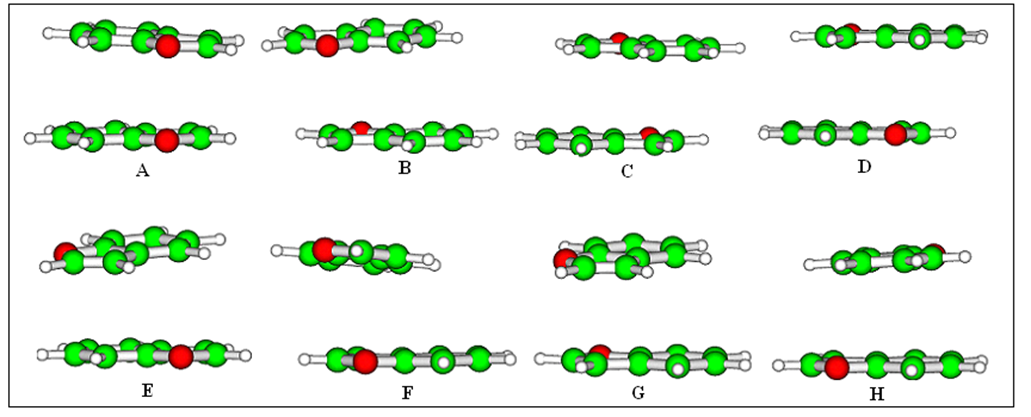
\includegraphics[scale=0.8]{image/Benzof-di}
\end{center}
	\caption{}Configurations of benzofuran dimers optimized at the $\omega$B97X-D/6-311++G** level of theory.
\end{figure}


\begin{table}[htbp]
	\caption{Interaction energies of benzofuran dimers (kcal/mol) in 8 different configurations using $\omega$B97X-D/6-311++G**. and compared with other methods.}
	\begin{tabular}{ccccccccc}
		\toprule
		\multicolumn{1}{l}{} & \textbf{A} & \textbf{B} & \textbf{C} & \textbf{D} & \textbf{E} & \textbf{F} & \textbf{G} & \textbf{H} \\ 
		\midrule
		\textbf{$\omega$97X-D/
		6-311++G**} & -5.79 & -6.21 & -6.40 & -6.72 & \multicolumn{1}{l}{-6.28} & -6.50 & -6.40 & -6.52 \\ 
		\textbf{DFT-SAPT(PBE0)
		aug-ccpvtz} & -4.47 & -4.81 & -5.00 & -5.29 & -4.84 & -5.24 & -4.91 & -4.99 \\ 
		\textbf{LMP2/ aug-ccpvtz}$^{a}$ & -4.60 &  &  &  &  &  &  &  \\ 
		\bottomrule
	\end{tabular}
	\label{}
\end{table}



\begin{table}[htbp]
	\caption{Intermolecular distance between furan rings center of benzofuran dimers (Å)}
	\begin{tabular}{cllllllll}
		\toprule
		\multicolumn{1}{l}{} & \multicolumn{1}{c}{\textbf{A}} & \multicolumn{1}{c}{\textbf{B}} & \multicolumn{1}{c}{\textbf{C}} & \multicolumn{1}{c}{\textbf{D}} & \multicolumn{1}{c}{\textbf{E}} & \multicolumn{1}{c}{\textbf{F}} & \multicolumn{1}{c}{\textbf{G}} & \multicolumn{1}{c}{\textbf{H}} \\ 
		\midrule
		\textbf{$\omega$B97x-D/
			6-311++G**} & 3.84 & 3.61 & 3.52 & 3.65 &4.37  & 3.46 & 3.68 & 4.08 \\ 
		\textbf{DFT-SAPT(PBE0)/
			aug-ccpvtz} & 3.86 & 3.63 & 3.53 & 3.65 & 4.39 & 3.47 & 3.71 & 4.08 \\ 
		\bottomrule
	\end{tabular}
	\label{}
\end{table}


\begin{table}[htbp]
	\caption{Angle between ring planes of benzofuran dimers ($^{\circ}$) at the $\omega$B97x-D/6-311++G** level of theory. according to figure }
	\begin{center}
	\begin{tabular}{cllllllll}
		\toprule
				& \multicolumn{1}{c}{\textbf{A}} & \multicolumn{1}{c}{\textbf{B}} & \multicolumn{1}{c}{\textbf{C}} & \multicolumn{1}{c}{\textbf{D}} & \multicolumn{1}{c}{\textbf{E}} & \multicolumn{1}{c}{\textbf{F}} & \multicolumn{1}{c}{\textbf{G}} & \multicolumn{1}{c}{\textbf{H}} \\ 
				\midrule
		\textbf{$\alpha$
		} & 18.10 & 4.12 & 9.26 & 5.80 & 9.82 & 6.47 & 5.54 & 9.89 \\ 
		\textbf{$\beta$
		} & 14.08 & 5.53 & 6.98 & 4.08 & 9.17 & 4.87 & 9.02 & 9.58 \\ 
		\textbf{$\gamma$
		} & \multicolumn{1}{c}{} & \multicolumn{1}{c}{} & \multicolumn{1}{c}{} & \multicolumn{1}{c}{} & \multicolumn{1}{c}{63.58} & \multicolumn{1}{c}{100.73} & \multicolumn{1}{c}{61.49} & \multicolumn{1}{c}{81.51} \\ 
		\bottomrule
	\end{tabular}
\end{center}
	\label{}
\end{table}

	\begin{table}[H]
		\caption{Calculated low wavenumber Raman ad PA infrared spectra of Benzofuran Dimer.}
		\begin{center}
			\begin{threeparttable}
				\begin{tabular}{c c c c c c c c}
					\toprule
					\textbf{Mode} & \textbf{$\omega$ cm$^{-1}$} & \multicolumn{1}{p{3cm}}{\centering \textbf{Intensities} \\ \textbf{($^{a}$) [$^{b}$]}}&  &  & \textbf{Mode} & \textbf{$\omega$ cm$^{-1}$} & \multicolumn{1}{p{3cm}}{\centering \textbf{Intensities} \\ \textbf{($^{a}$) [$^{b}$]}}\\
					\midrule
$\nu_{1}$& 16 & (0.13)    [0.00] & & &$\nu_{12}$&  413 & (8.20)  [0.00] \\ 
$\nu_{2}$& 33 & (0.00)    [7.09] && &  $\nu_{13}$&  433 & (20.00)  [0.00] \\ 
$\nu_{3}$&  60 & (0.00)   [7.03] & && $\nu_{14}$& 435 & (0.00)   [1.23] \\ 
$\nu_{4}$&  69 & (0.80)   [0.00] &&& $\nu_{15}$&  553 & (1.18)  [0.01] \\ 
$\nu_{5}$&  73 & (0.34)   [0.00] &&& $\nu_{16}$&  553 & (0.00)  [10.7] \\ 
$\nu_{6}$&  93 & (0.00)    [4.56] &&& $\nu_{17}$&  587 & (0.95)  [0.00] \\ 
$\nu_{7}$&  229 & (0.002)  [1.03] &&& $\nu_{18}$ & 588 & (0.00)  [0.47]\\ 
$\nu_{8}$&  232 & (15.24)  [0.00] &&& $\nu_{19}$ & 602 & (0.00)  [3.35] \\ 
$\nu_{9}$&  258 & (2.59)  [0.00] &&& $\nu_{20}$&  605 & (1.26)  [0.00] \\ 
$\nu_{10}$&  263 & (0.00) [0.93] &&& $\nu_{21}$ & 628 & (0.00)  [10.86] \\ 
$\nu_{11}$&  413 & (0.01)  [0.27] &&& $\nu_{22}$ & 628 & (2.02)  [0.00] \\ 
	\bottomrule
\end{tabular}

\begin{tablenotes}
	\item[a] km/mole
	\item[b] A$^{4}$/AMU
\end{tablenotes}
\end{threeparttable}
\end{center}
\label{low-freqBnzfDi}
\end{table}



\begin{table}[H]
	\caption{Raman ad PA infrared spectra of Benzofuran Dimer, 700- 2000 cm$^{-1}$}
	\begin{center}
			\begin{tabular}{c c c c c c c c }
				\toprule
				\textbf{Mode} &\textbf{$\omega$ cm$^{-1}$} & \multicolumn{1}{p{3cm}}{\centering \textbf{Intensities} \\ \textbf{($^{a}$) [$^{b}$]}}&  &  & \textbf{Mode} & \textbf{$\omega$ cm$^{-1}$} & \multicolumn{1}{p{3cm}}{\centering \textbf{Intensities} \\ \textbf{($^{a}$) [$^{b}$]}}\\
				\midrule
$\nu_{23}$ & 751 & (0.003)  [1.11] &  &  & $\nu_{43}$ & 1042 & (10.47)  [0.05] \\ 
$\nu_{24}$ & 755 & (23.17)  [0.00] &  &  & $\nu_{44}$ & 1042 & (0.01)  [42.05] \\ 
$\nu_{25}$ & 771 & (243.20) [0.00] &  &  & $\nu_{45}$ & 1073 & (0.00)  [17.51] \\ 
$\nu_{26}$ & 774 & (0.006)  [0.44] &  &  & $\nu_{46}$ & 1074 & (20.96)  [0.00] \\ 
$\nu_{27}$ & 789 & (11.41)  [0.00] &  &  & $\nu_{47}$ & 1136 & (0.003)  [6.05] \\ 
$\nu_{28}$ & 789 & (0.00)  [36.07] &  &  & $\nu_{48}$ & 1137 & (21.91)  [0.00] \\ 
$\nu_{29}$ & 792 & (42.03)  [0.00] &  &  & $\nu_{49}$ & 1165 & (31.38)  [0.00] \\ 
$\nu_{30}$ & 793 & (0.06) [0.47] &  &  & $\nu_{50}$&  1166 & (0.00)  [10.5] \\ 
$\nu_{31}$ & 878 & (0.00)  [0.49] &  &  & $\nu_{51}$&  1182 & (0.00)  [3.39] \\ 
$\nu_{32}$ & 878 & (2.03)  [0.00] &  &  & $\nu_{52}$&  1183 & (5.03)  [0.00] \\ 
$\nu_{33}$ & 882 & (0.00)  [4.95] &  &  & $\nu_{53}$&  1212 & (0.02)  [2.15] \\ 
$\nu_{34}$ & 882 & (13.55)  [0.00] &  &  & $\nu_{54}$&  1212 & (34.44)  [0.001] \\ 
$\nu_{35}$ & 897 & (0.04)  [6.85] &  &  & $\nu_{55}$&  1299 & (0.002)  [28.04] \\ 
$\nu_{36}$ & 897 & (5.37)  [0.04] &  &  & $\nu_{56}$&  1300 & (9.36)  [0.01] \\ 
$\nu_{37}$ & 922 & (0.005) [0.01] &  &  & $\nu_{57}$&  1301 & (0.00)  [48.82] \\ 
$\nu_{38}$ & 922 & (5.15)  [0.01] &  &  & $\nu_{58}$&  1305 & (58.62)  [0.00] \\ 
$\nu_{39}$ & 964 & (6.58)  [0.00] &  &  & $\nu_{59}$&  1371 & (9.76)  [0.001] \\ 
$\nu_{40}$ & 965 & (0.00)  [0.21] &  &  & $\nu_{60}$&  1373 & (0.00)  [28.56] \\ 
$\nu_{41}$ & 997 & (0.00)  [0.49] &  &  & $\nu_{61}$&  1396 & (3.53)  [0.001] \\ 
$\nu_{42}$ & 998 & (0.26)  [0.00] &  &  & $\nu_{62}$&  1396 & 0.00)  [20.70] \\ 
	\bottomrule
\end{tabular}
\end{center}
\end{table}



\begin{table}[H]
	\begin{center}
		\begin{threeparttable}
		\begin{tabular}{c c c c c c c c}
			\toprule
			\textbf{Mode} & \textbf{$\omega$ cm$^{-1}$} & \multicolumn{1}{p{3cm}}{\centering \textbf{Intensities} \\ \textbf{($^{a}$) [$^{b}$]}}&  &  & \textbf{Mode} & \textbf{$\omega$ cm$^{-1}$} & \multicolumn{1}{p{3cm}}{\centering \textbf{Intensities} \\ \textbf{($^{a}$) [$^{b}$]}}\\
			\midrule
$\nu_{63}$&  1502 & (76.23)  0.003 &  &  & $\nu_{68}$&  1609 & (24.08)  0.00 \\ 
$\nu_{64}$&  1503 & (0.02)  10,81 &  &  & $\nu_{69}$&  1664 & (0.18)  0.01 \\ 
$\nu_{65}$&  1524 & (7.06)  0.002 &  &  & $\nu_{70}$&  1664 & (0.00)  15.60 \\ 
$\nu_{66}$&  1525 & (0.002)  8,11 &  &  & $\nu_{71}$&  1691 & 0.50)  0.96 \\ 
$\nu_{67}$&  1608 & (0.00)  143.49 &  &  & $\nu_{72}$&  1691 & (0.008) 65.93 \\ 

	\bottomrule
\end{tabular}

\begin{tablenotes}
	\item[a] km/mole
	\item[b] A$^{4}$/AMU
\end{tablenotes}
\end{threeparttable}
\end{center}
\label{freqBnzfDi}
\end{table}


\begin{figure}[H]
	\begin{center}
		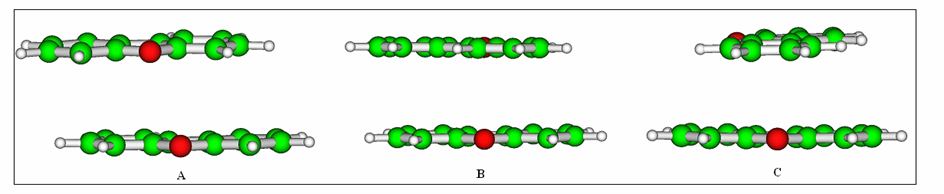
\includegraphics[scale=0.9]{image/dibenf-dim}
	\end{center}
	\caption{Configurations of dibenzofuran dimers optimized at the $\omega$B97x-D/6-311++G** level of theory.}
\end{figure}

\begin{table}[htbp]
	\caption{Interaction energies of dibenzofuran dimers (kcal/mol) in 3 different configurations using $\omega$B97x-D/6-311++G**.}
		\begin{center}
	\begin{tabular}{cccc}
		\toprule
		& \textbf{A} & \textbf{B} & \textbf{C} \\ 
		\midrule
		\textbf{$\omega$B97x-D/
		6-311++G** }& -10.03	& -10.38	& -9.58	\\ 
	\bottomrule
	\end{tabular}
\end{center}
	\label{}
\end{table}


\begin{table}[htbp]
	\caption{ntermolecular distance between furan ring center (Å) according figure of dibenzofuran dimers using $\omega$B97x-D/6-311++G**.}
	\begin{center}
		\begin{tabular}{cccc}
			\toprule
			& \textbf{A} & \textbf{B} & \textbf{C} \\ 
			\midrule
			\textbf{d}& 3.67	& 3.82	& 3.39\\ 
			\bottomrule
		\end{tabular}
	\end{center}
	\label{}
\end{table}



\begin{table}[H]
	\caption{Calculated low wavenumber Raman ad PA infrared spectra of Dibenzofuran Dimer.}
	\begin{center}
		\begin{threeparttable}
			\begin{tabular}{c c c c c c c c}
				\toprule
				\textbf{Mode} & \textbf{$\omega$ cm$^{-1}$} & \multicolumn{1}{p{3cm}}{\centering \textbf{Intensities} \\ \textbf{($^{a}$) [$^{b}$]}}&  &  & \textbf{Mode} & \textbf{$\omega$ cm$^{-1}$} & \multicolumn{1}{p{3cm}}{\centering \textbf{Intensities} \\ \textbf{($^{a}$) [$^{b}$]}}\\
				\midrule
$\nu_{1}$&  12 & (0.03)  [2.29] &  &  & $\nu_{18}$&  436 & (1.47)  [5.71] \\ 
$\nu_{2}$&  27 & (0.04)  [5.45] &  &  & $\nu_{19}$&  436 & (1.41)  [7.34] \\ 
$\nu_{3}$&  37 & (0.09)  [9.99] &  &  & $\nu_{20}$&  437 & (2.71)  [1.85] \\ 
$\nu_{4}$&  63 & (0.5) [0.69] &  &  & $\nu_{21}$ & 447 & (0.12)  [0.38] \\ 
$\nu_{5}$&  78 & (0.26)  [1.31] &  &  & $\nu_{22}$ & 449 & (0.19)  [0.41] \\ 
$\nu_{6}$&  88 & (0.08)  [1.92] &  &  & $\nu_{23}$ & 531 & (0.01)  [2.63] \\ 
$\nu_{7}$&  121 & (4.03)  [0.50] &  &  & $\nu_{24}$ & 532 & (0.20)  [1.01] \\ 
$\nu_{8}$& 126 & (0.04)  [1.14 &  &  & $\nu_{25}$ & 573 & (3.35)  [4.98] \\ 
$\nu_{9}$&  163 & (0.04)  [0.36 &  &  & $\nu_{26}$ & 573 & (1.76)  [6.88] \\ 
$\nu_{10}$&  167 & (0.06)  [0.32] &  &  & $\nu_{27}$ & 580 & (1.47) [0.31] \\ 
$\nu_{11}$&  222 & (0.34)  [1.09] &  &  & $\nu_{28}$ & 580 & (7.51) [0.38] \\ 
$\nu_{12}$&  222 & (1.52)  [0.31] &  &  & $\nu_{29}$ & 586 & (0.15)  [0.16] \\ 
$\nu_{13}$&  299 & (0.05)  [6.95] &  &  & $\nu_{30}$ & 587 & (0.01)  [0.02] \\ 
$\nu_{14}$&  302 & (0.10)  [1.37] &  &  & $\nu_{31}$ & 633 & (0.86)  [0.05] \\ 
$\nu_{15}$&  321 & (0.28)  [0.09] &  &  & $\nu_{32}$ & 634 & (7.41)  [0.01] \\ 
$\nu_{16}$& 323 & (0.02)  [1.90] &  &  & $\nu_{33}$ & 678 & (0.08)  [1.58] \\ 
$\nu_{17}$&  434 & (10.51) [0.60] &  &  & $\nu_{31}$ & 679 & (1.07)  [0.12] \\ 
	\bottomrule
\end{tabular}

\begin{tablenotes}
	\item[a] km/mole
	\item[b] A$^{4}$/AMU
\end{tablenotes}
\end{threeparttable}
\end{center}
\label{low-freqDibenzofDi}
\end{table}


\begin{table}[H]
	\caption{Raman ad PA infrared spectra of Dibenzofuran Dimer, 700- 2000 cm$^{-1}$}
	\begin{center}
		\begin{tabular}{c c c c c c c c }
			\toprule
			\textbf{Mode} &\textbf{$\omega$ cm$^{-1}$} & \multicolumn{1}{p{3cm}}{\centering \textbf{Intensities} \\ \textbf{($^{a}$) [$^{b}$]}}&  &  & \textbf{Mode} & \textbf{$\omega$ cm$^{-1}$} & \multicolumn{1}{p{3cm}}{\centering \textbf{Intensities} \\ \textbf{($^{a}$) [$^{b}$]}}\\
			\midrule
$\nu_{32}$ & 746 & (140.16)  [0.05] &  &  & $\nu_{46}$ & 874 & (0.48) [0.36] \\ 
$\nu_{33}$ & 748 & (2.57)  [0.45] &  &  & $\nu_{47}$&  876 & (0.37)  [5.56] \\ 
$\nu_{32}$ & 763 & (0.39)  [0.64] &  &  & $\nu_{48}$&  876 & (12.21)  [5.69] \\ 
$\nu_{33}$ & 766 & (4.67)  [0.11] &  &  & $\nu_{49}$&  877 & (10.55)  [1.63] \\ 
$\nu_{32}$ & 767 & (0.56)  [2.67] &  &  & $\nu_{50}$&  877 & (23.66)  [8.54] \\ 
$\nu_{33}$ & 768 & 0.02)  [39.98] &  &  & $\nu_{51}$&  878 & (3.55)  [6.61] \\ 
$\nu_{32}$ & 774 & (0.20)  [2.90] &  &  & $\nu_{52}$&  879 & (4.99)  [0.55] \\ 
$\nu_{33}$ & 776 & (27.11) [0.30] &  &  & $\nu_{53}$&  962 & (4.95)  [0.25] \\ 
$\nu_{43}$&  777 & (180.51)  [180,51] &  &  & $\nu_{54}$ & 964 & (1.78)  [0.13] \\ 
$\nu_{44}$&  780 & (8.58)  [8,58] &  &  & $\nu_{55}$&  965 & (3.33)  [0.18] \\ 
$\nu_{45}$&	873&	(4.45)	[4,45]& & & $\nu_{56}$&	966	&(0.43)	[0.21]\\
 	\bottomrule
\end{tabular}
\end{center}
\end{table}



\begin{table}[H]
	\begin{center}
		\begin{threeparttable}
			\begin{tabular}{c c c c c c c c}
				\toprule
				\textbf{Mode} & \textbf{$\omega$ cm$^{-1}$} & \multicolumn{1}{p{3cm}}{\centering \textbf{Intensities} \\ \textbf{($^{a}$) [$^{b}$]}}&  &  & \textbf{Mode} & \textbf{$\omega$ cm$^{-1}$} & \multicolumn{1}{p{3cm}}{\centering \textbf{Intensities} \\ \textbf{($^{a}$) [$^{b}$]}}\\
				\midrule
	$\nu_{56}$&  966 & (0.43)  [0.21] &  &  & $\nu_{81}$&  1316 & (6.02)  [1.48] \\ 
	$\nu_{57}$&  996 & (0.23)  [0.31] &  &  & $\nu_{82}$&  1316 & (26.74) [1.35] \\ 
	$\nu_{58}$&  997 & (0.18) [0.11] &  &  & $\nu_{83}$&  1343 & (1.77)  [66.22] \\ 
	$\nu_{59}$&  999 & (0.05)  [0.24] &  &  & $\nu_{84}$&  1344 & (1.88)  [92.12] \\ 
	$\nu_{60}$&  1000 & (0.18)  [0.14] &  &  & $\nu_{85}$&  1368 & (17.78)  [0.90] \\ 
	$\nu_{61}$&  1031 & (0.08)  [1.49] &  &  & $\nu_{86}$&  1368 & (3.08)  [2.31] \\ 
	$\nu_{62}$&  1032 & (1.08)  [0.16] &  &  & $\nu_{87}$&  1389 & (4.41))  (26.90) \\ 
	$\nu_{63}$&  1045 & (0.81) [2.21] &  &  & $\nu_{88}$& 1390 & (3.81)  [24.86] \\ 
	$\nu_{64}$&  1045 & (0.09)  [81.70] &  &  & $\nu_{89}$&  1493 & (47.13) [8.24] \\ 
	$\nu_{65}$&  1052 & (3.86)  [0.18] &  &  & $\nu_{90}$&  1494 & (18.13) [19.34] \\ 
	$\nu_{66}$&  1052 & (17.66)  [0.05] &  &  & $\nu_{91}$&  1500 & (45.74)  [0.63] \\ 
	$\nu_{67}$&  1135 & (1.19)  [10.14] &  &  & $\nu_{92}$&  1500 & (11.05)  [1.09] \\ 
	$\nu_{68}$&  1135 & (14.60)  [0.54] &  &  & $\nu_{93}$&  1522 & (11.12)  [8.31] \\ 
	$\nu_{69}$&  1146 & (1.53)  [4.05] &  &  & $\nu_{94}$&  1522 & (67.33)  [4.38] \\ 
	$\nu_{70}$&  1146 & (9.83)  [1.44] &  &  & $\nu_{95}$&  1542 & (0.44)  [54.73] \\ 
	$\nu_{71}$&  1178 & (1.34)  [12.15] &  &  & $\nu_{96}$&  1543 & (1.04)  [6.90] \\ 
	$\nu_{72}$&  1179 & (2.83)  [8.51] &  &  & $\nu_{97}$&  1662 & (1.41)  [6.10] \\ 
	$\nu_{73}$&  1187 & (0.18)  [1.54] &  &  & $\nu_{98}$&  1662 & (11.95)  [1.93] \\ 
	$\nu_{74}$&  1187 & (0.14)  [1.41] &  &  & $\nu_{99}$&  1668 & (0.41)  [17.86] \\ 
	$\nu_{75}$&  1232 & (1.15)  [13.45] &  &  & $\nu_{100}$ & 1668 & (1.61)  [9.85] \\ 
	$\nu_{76}$&  1233 & (2.12)  [5.32] &  &  & $\nu_{101}$&  1675 & (1.42)  [3.71] \\ 
	$\nu_{77}$&  1244 & (27.73)  [6.88] &  &  & $\nu_{102}$&  1675 & (15.67)  [1.05] \\ 
	$\nu_{78}$&  1249 & (205.63) [2.36] &  &  & $\nu_{103}$&  1713 & (0.23)  [269.45] \\ 
	$\nu_{79}$&  1290 & (4.37)  [123.94] &  &  & $\nu_{104}$&  1713 & (0.50)  [199.85] \\ 			
		\bottomrule
\end{tabular}

\begin{tablenotes}
	\item[a] km/mole
	\item[b] A$^{4}$/AMU
\end{tablenotes}
\end{threeparttable}
\end{center}
\label{freqDibenfDi}
\end{table}
				
				
				
				

\begin{figure}[H]
	\begin{center}
		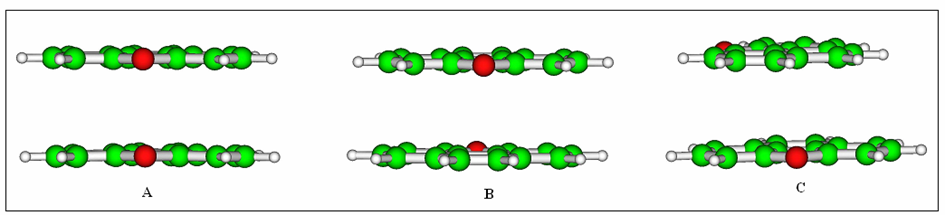
\includegraphics[scale=0.9]{anex/image/tribenzof-dim}
	\end{center}
	\caption{Configurations of Tribenzofuran dimers optimized at the $\omega$B97x-D/6-311++G** level of theory.}
\end{figure}


\begin{table}[htbp]
	\caption{Interaction energies of Tribenzofuran dimers (kcal/mol) in 3 different configurations using $\omega$B97x-D/6-311++G**.}
	\begin{center}
		\begin{tabular}{cccc}
			\toprule
			& \textbf{A} & \textbf{B} & \textbf{C} \\ 
			\midrule
			\textbf{$\omega$B97x-D/
				6-311++G** }& -12.31	& -13.30	& -13.58	\\ 
			\bottomrule
		\end{tabular}
	\end{center}
	\label{}
\end{table}


\begin{table}[htbp]
	\caption{ntermolecular distance between furan ring center (Å) according figure of Tribenzofuran dimers using $\omega$B97x-D/6-311++G**.}
	\begin{center}
		\begin{tabular}{cccc}
			\toprule
			& \textbf{A} & \textbf{B} & \textbf{C} \\ 
			\midrule
			\textbf{d}& 3.68	& 4.71	& 4.25\\ 
			\bottomrule
		\end{tabular}
	\end{center}
	\label{}
\end{table}


\begin{table}[H]
	\caption{Calculated low wavenumber Raman ad PA infrared spectra of Tribenzofuran Dimer.}
	\begin{center}
		\begin{threeparttable}
			\begin{tabular}{c c c c c c c c}
				\toprule
				\textbf{Mode} & \textbf{$\omega$ cm$^{-1}$} & \multicolumn{1}{p{3cm}}{\centering \textbf{Intensities} \\ \textbf{($^{a}$) [$^{b}$]}}&  &  & \textbf{Mode} & \textbf{$\omega$ cm$^{-1}$} & \multicolumn{1}{p{3cm}}{\centering \textbf{Intensities} \\ \textbf{($^{a}$) [$^{b}$]}}\\
				\midrule
$\nu_{1}$&  21 & (0.05)  [2.13] &  &  & $\nu_{21}$&  457 & (0.04)  [16.62] \\ 
$\nu_{2}$&  23 & (0.16)  [11.11] &  &  & $\nu_{22}$ & 458 & (0.01)  [17.46] \\ 
$\nu_{3}$&  49 & (0.00)  [9.65] &  &  & $\nu_{23}$ & 491 & (1.36)  [1.74] \\ 
$\nu_{4}$&  77 & (0.40)  [0.19] &  &  & $\nu_{24}$ & 491 & (1.93)  [3.62] \\ 
$\nu_{5}$&  79 & (0.01)  [2.70] &  &  & $\nu_{25}$ & 504 & (0.29)  [0.34] \\ 
$\nu_{6}$&  92 & (3.12)  [1.14] &  &  & $\nu_{26}$ & 506 & (8.12)  [0.03] \\ 
$\nu_{7}$&  98 & (4.42)  [1.12] &  &  & $\nu_{27}$ & 557 & (0.40)  [2.18] \\ 
$\nu_{8}$&  119 & (0.00)  [3.63] &  &  & $\nu_{28}$&  558 & (0.45)  [2.84] \\ 
$\nu_{9}$&  200 & (0.03)  [0.18] &  &  & $\nu_{29}$ & 576 & (0.004)  [0.09] \\ 
$\nu_{10}$&  212 & (0.01)  [1.01] &  &  & $\nu_{30}$ & 578 & (0.003)  [0.28] \\ 
$\nu_{11}$&  222 & (0.08)  [2.53] &  &  & $\nu_{31}$ & 585 & (2.60)  [0.57] \\ 
$\nu_{12}$&  228 & (5.98)  [0.46] &  &  & $\nu_{32}$ & 586 & (2.93)  [0.77] \\ 
$\nu_{13}$&  307 & (0.21)  [1.72] &  &  & $\nu_{33}$ & 611 & (8.03)  [0.17] \\ 
$\nu_{14}$&  309 & (0.09)  [1.22] &  &  & $\nu_{34}$ & 612 & (0.40)  [0.11] \\ 
$\nu_{15}$&  326 & (0.62)  [1.06] &  &  & $\nu_{35}$ & 623 & (1.39)  [48.21] \\ 
$\nu_{16}$&  329 & (0.11)  [1.82] &  &  & $\nu_{36}$ & 624 & (2.54)  [0.54] \\ 
$\nu_{17}$&  348 & (3.43)  [0.30] &  &  & $\nu_{37}$ & 663 & (0.09)  [0.11] \\ 
$\nu_{18}$&  348 & (4.57)  [0.26] &  &  & $\nu_{38}$ & 663 & (0.19)  [0.58] \\ 
$\nu_{19}$&  437 & (0.09) [1.52] &  &  & $\nu_{39}$ & 690 & (0.63)  [0.15] \\ 
$\nu_{20}$&  439 & (0.02)  [2.40] &  &  & $\nu_{40}$ & 691 & (0.30)  [13.37] \\ 
	\bottomrule
\end{tabular}

\begin{tablenotes}
	\item[a] km/mole
	\item[b] A$^{4}$/AMU
\end{tablenotes}
\end{threeparttable}
\end{center}
\label{low-freqTribenzofDi}
\end{table}



\begin{table}[H]
	\caption{Raman ad PA infrared spectra of Dibenzofuran Dimer, 700- 2000 cm$^{-1}$}
	\begin{center}
		\begin{threeparttable}
		\begin{tabular}{c c c c c c c c }
			\toprule
			\textbf{Mode} &\textbf{$\omega$ cm$^{-1}$} & \multicolumn{1}{p{3cm}}{\centering \textbf{Intensities} \\ \textbf{($^{a}$) [$^{b}$]}}&  &  & \textbf{Mode} & \textbf{$\omega$ cm$^{-1}$} & \multicolumn{1}{p{3cm}}{\centering \textbf{Intensities} \\ \textbf{($^{a}$) [$^{b}$]}}\\
			\midrule
$\nu_{41}$ & 707 & (1.30)  [0.10] &  &  & $\nu_{79}$&  1196 & (2.85)  [0.37] \\ 
$\nu_{42}$ & 707 & (1.01)  [0.08] &  &  & $\nu_{80}$&  1196 & (4.37)  [0.89] \\ 
$\nu_{43}$ & 734 & (91.56)  [0.03] &  &  & $\nu_{81}$&  1205 & (0.00)  [0.55] \\ 
$\nu_{44}$ & 735 & (0.70)  [0.38] &  &  & $\nu_{82}$&  1206 & (0.003)  [0.51] \\ 
$\nu_{45}$ & 767 & (1.42)  [0.20] &  &  & $\nu_{83}$&  1243 & (6.01)  [998.56] \\ 
$\nu_{46}$ & 768 & (2.08)  [0.16] &  &  & $\nu_{84}$&  1243 & (10.43)  [24.23] \\ 
$\nu_{47}$ & 775 & (12.66)  [0.13] &  &  & $\nu_{85}$&  1253 & (2.95)  [0.48] \\ 
$\nu_{48}$&  776 & (64.56)  [0.12] &  &  & $\nu_{86}$ & 1254 & (0.06)  [8.25] \\ 
$\nu_{49}$&  808 & (0.58)  [1.90] &  &  & $\nu_{87}$&  1257 & (9.46)  [2.56] \\ 
$\nu_{50}$&  208 & (2.49)  [1.20] &  &  & $\nu_{88}$&  1258 & (20.06)  [7.40] \\ 
$\nu_{51}$&  815 & (3.45)  [0.92] &  &  & $\nu_{89}$&  1274 & (16.27) [0.49] \\ 
$\nu_{52}$&  815 & (5.20)  [1.93] &  &  & $\nu_{90}$&  1275 & (35.04)  [3.28] \\ 
$\nu_{53}$&  838 & (3.35)  [7.73] &  &  & $\nu_{91}$&  1352 & (16.11)  [42.19] \\ 
$\nu_{54}$&  839 & (3.04)  [10.57] &  &  & $\nu_{92}$&  1352 & (10.15)  [62.41] \\ 
$\nu_{55}$&  842 & (173.42)  [0.30] &  &  & $\nu_{93}$&  1403 & (1.25)  [5.26] \\ 
$\nu_{56}$&  845 & (29.05)  [0.72] &  &  & $\nu_{94}$&  1404 & (3.42)  [14.86] \\ 
$\nu_{57}$&  906 & (0.12)  [0.48] &  &  & $\nu_{95}$&  1405 & (8.16)  [0.72] \\ 
$\nu_{58}$&  907 & (0.03)  [0.56] &  &  & $\nu_{96}$&  1407 & (19.96)  [0.53] \\ 
$\nu_{59}$&  913 & (3.04)  [0.23] &  &  & $\nu_{97}$&  1441 & (0.28)  [15.89] \\ 
$\nu_{60}$&  914 & (3.85)  [0.27] &  &  & $\nu_{98}$&  1442 & (0.33)  [25.67] \\ 
$\nu_{61}$&  987 & (0.61)  [0.13] &  &  & $\nu_{99}$&  1467 & (34.56)  [0.39] \\ 
$\nu_{62}$&  987 & (0.15)  [0.04] &  &  & $\nu_{100}$&  1467 & (20.10)  [0.61] \\ 
$\nu_{63}$&  989 & (0.35)  [0.06] &  &  & $\nu_{101}$&  1491 & (20.89)  [5.82] \\ 
$\nu_{64}$&  989 & (3.52)  [0.02] &  &  & $\nu_{102}$& 1492 & (11.19)  [34.98] \\ 
$\nu_{65}$&  998 & (1.54)  [1.93] &  &  & $\nu_{103}$&  1535 & (0.003)  [361.12] \\ 
$\nu_{66}$&  1000 & (1.47)  [2.13] &  &  & $\nu_{104}$&  1536 & (0.24)  [50.34] \\ 
$\nu_{67}$&  1025 & (5.30)  [1.67] &  &  & $\nu_{105}$&  1543 & (0.11  [0.83] \\ 
$\nu_{68}$&  1026 & (3.01)  [1.85] &  &  & $\nu_{106}$&  1543 & (0.25)  [2.20] \\ 
$\nu_{69}$&  1027 & (7.67)  [2.94] &  &  & $\nu_{107}$&  1563 & (12.63)  [2.49] \\ 
$\nu_{70}$&  1028 & (0.23)  [0.37] &  &  & $\nu_{108}$&  1564 & (21.52)  [0.59] \\ 
$\nu_{71}$&  1045 & (0.14)  [48.95] &  &  & $\nu_{109}$&  1657 & (34.71)  [0.18] \\ 
$\nu_{72}$&  1046 & (0.47)  [12.77] &  &  & $\nu_{110}$&  1658 & (67.22)  [3.42] \\ 
$\nu_{73}$&  1071 & (19.53)  [0.67] &  &  & $\nu_{111}$&  1699 & (0.82)  [29.36] \\ 
$\nu_{74}$&  1072 & (24.13)  [2.47] &  &  & $\nu_{112}$&  1699 & (1.19)  [16.13] \\ 
$\nu_{75}$&  1075 & (32.97)  [0.31] &  &  & $\nu_{113}$&  1722 & (1.37)  [70.71] \\ 
$\nu_{76}$&  1075 & (72.14)  [1.23] &  &  & $\nu_{114}$&  1722 & (0.74)  [38.60] \\ 
$\nu_{77}$&  1165 & (0.21)  [3.04] &  &  & $\nu_{115}$&  1752 & (0.06)  [23.64] \\ 
$\nu_{78}$&  1166 & (0.89)  [0.35] &  &  & $\nu_{116}$&  1753 & (0.58)  [26.38] \\ 
\bottomrule
\end{tabular}

\begin{tablenotes}
	\item[a] km/mole
	\item[b] A$^{4}$/AMU
\end{tablenotes}
\end{threeparttable}
\end{center}
\label{freqTribenzofDi}
\end{table}

\begin{figure}[H]
	\begin{center}
		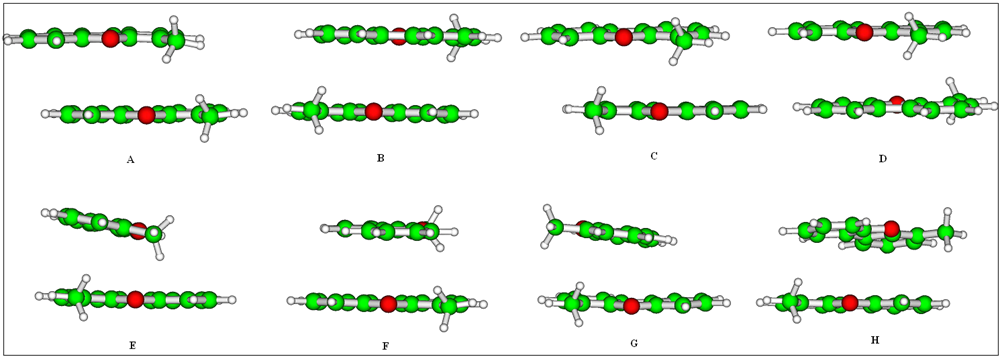
\includegraphics[scale=0.8]{image/4-mO-dim}
	\end{center}
	\caption{Configurations of 4-methyldibenzofuran dimers optimized at the $\omega$B97x-D/6-311++G** level of theory.}
\end{figure}

\begin{table}[H]
	\caption{Interaction energies of  4-methyldibenzofuran dimers (kcal/mol) using $\omega$B97X-D/6-311++G**.}
	\begin{center}
		\begin{tabular}{c c c c c c c c c}
			\hline
			& \textbf{A} & \textbf{B} & \textbf{C} & \textbf{D} & \textbf{E} & \textbf{F} & \textbf{G} & \textbf{H} \\ \hline
			\textbf{$\omega$B97X-D/
				6-311++G**} & -11.54 & -11.74 & -11.59 & -11.29 & -12.67 & -12.30 & -12.79 & -11.87 \\ \hline
		\end{tabular}
	\end{center}
	\label{}
\end{table}


\begin{figure}[H]
	\begin{center}
		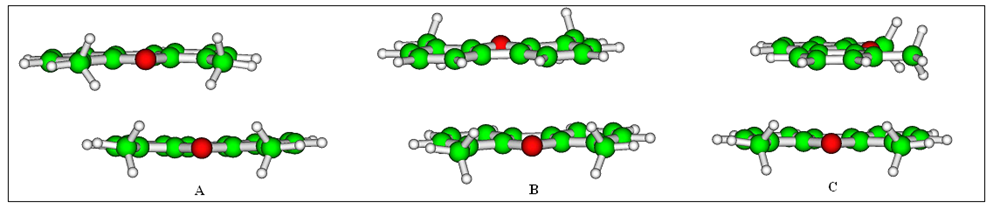
\includegraphics[scale=0.9]{image/46-dmdibf-dim}
	\end{center}
	\caption{Configurations of 4,6-dimethyldibenzofuran dimers optimized at the $\omega$B97x-D/6-311++G** level of theory.}
\end{figure}


\begin{table}[htbp]
	\caption{Interaction energies of 4,6-dimethyldibenzofuran dimers (kcal/mol) in 3 different configurations using $\omega$B97x-D/6-311++G**.}
	\begin{center}
		\begin{tabular}{cccc}
			\toprule
			& \textbf{A} & \textbf{B} & \textbf{C} \\ 
			\midrule
			\textbf{$\omega$B97x-D/
				6-311++G** }& -13.32	& -13.74	& -13.63	\\ 
			\bottomrule
		\end{tabular}
	\end{center}
	\label{}
\end{table}


\begin{table}[H]
	\caption{Calculated low wavenumber Raman ad PA infrared spectra of 4,6-dimethyldibenzofuran Dimer.}
	\begin{center}
		\begin{threeparttable}
			\begin{tabular}{c c c c c c c c}
				\toprule
				\textbf{Mode} & \textbf{$\omega$ cm$^{-1}$} & \multicolumn{1}{p{3cm}}{\centering \textbf{Intensities} \\ \textbf{($^{a}$) [$^{b}$]}}&  &  & \textbf{Mode} & \textbf{$\omega$ cm$^{-1}$} & \multicolumn{1}{p{3cm}}{\centering \textbf{Intensities} \\ \textbf{($^{a}$) [$^{b}$]}}\\
				\midrule
$\nu_{1}$&  15 & (0.01)  [0.00] &  &  & $\nu_{24}$ & 309 & (0.40)  [0.00] \\ 
$\nu_{2}$&  24 & (0.00)  [6.54] &  &  & $\nu_{25}$ & 319 & (0.00)  [6.38] \\ 
$\nu_{3}$&  39 & (0.00)  [7.95] &  &  & $\nu_{26}$ & 319 & (0.22)  [0.00] \\ 
$\nu_{4}$&  78 & (0.05)  [0.00] &  &  & $\nu_{27}$ & 341 & (3.68)  [0.00] \\ 
$\nu_{5}$&  79 & (0.40)  [0.00] &  &  & $\nu_{28}$&  345 & (0.00)  [3.36] \\ 
$\nu_{6}$&  90 & (0.00)  [1.58] &  &  & $\nu_{29}$ & 472 & (4.21)  [0.00] \\ 
$\nu_{7}$&  99 & (0.12)  [0.00] &  &  & $\nu_{30}$ & 472 & (0.00)  [3.31] \\ 
$\nu_{8}$&  102 & (0.00) [0.27] &  &  & $\nu_{31}$ & 493 & (0.00)  [5.85] \\ 
$\nu_{9}$&  111 & (0.001)  [1.7] &  &  & $\nu_{32}$ & 493 & (0.03)  [0.00] \\ 
$\nu_{10}$& 111 & (5.17)  [0.00] &  &  & $\nu_{33}$ & 507 & (0.00)  [2.00] \\ 
$\nu_{11}$&  120 & (0.18)  [0.00] &  &  & $\nu_{34}$ & 510 & (4.30)  [0.00] \\ 
$\nu_{12}$&  141 & (0.00)  [1.24] &  &  & $\nu_{35}$ & 534 & (0.43)  [0.00] \\ 
$\nu_{13}$&  149 & (0.00)  [0.75] &  &  & $\nu_{36}$ & 536 & (0.00)  [0.43] \\ 
$\nu_{14}$&  150 & (0.70)  [0.00] &  &  & $\nu_{37}$ & 571 & (2.60)  [0.00] \\ 
$\nu_{15}$&  162 & (0.00)  [0.46] &  &  & $\nu_{38}$ & 571 & (0.00)  [36.63] \\ 
$\nu_{16}$&  163 & (1.17)  [0.00] &  &  & $\nu_{39}$ & 589 & (0.62)  [0.00] \\ 
$\nu_{17}$&  209 & (6.26)  [0.00] &  &  & $\nu_{40}$ & 589 & (0.00)  [0.25] \\ 
$\nu_{18}$&  221 & (0.00)  [1.98] &  &  & $\nu_{41}$ & 593 & (0.21)  [0.00] \\ 
$\nu_{19}$&  247 & (0.00)  [2.5] &  &  & $\nu_{42}$ & 594 & (0.00)  [0.99] \\ 
$\nu_{20}$&  259 & (0.35)  [0.00] &  &  & $\nu_{43}$ & 597 & (0.00)  [2.52] \\ 
$\nu_{21}$ & 268 & (0.00)  [3.52] &  &  & $\nu_{44}$ & 597 & (12.52)  [0.00] \\ 
$\nu_{22}$ & 268 & (1.88)  [0.00] &  &  & $\nu_{45}$ & 606 & (1.37)  [0.00] \\ 
$\nu_{23}$ & 305 & (0.00)  [4.76] &  &  & $\nu_{46}$ & 606 & (0.00)  [6.12] \\ 
	\bottomrule
\end{tabular}

\begin{tablenotes}
	\item[a] km/mole
	\item[b] A$^{4}$/AMU
\end{tablenotes}
\end{threeparttable}
\end{center}
\label{low-freq46-dmDibenzofDi}
\end{table}







\begin{table}[H]
	\caption{Raman ad PA infrared spectra of 4,6-dimethyldibenzofuran Dimer, 700- 2000 cm$^{-1}$}
	\begin{center}
		\begin{tabular}{c c c c c c c c }
			\toprule
			\textbf{Mode} &\textbf{$\omega$ cm$^{-1}$} & \multicolumn{1}{p{3cm}}{\centering \textbf{Intensities} \\ \textbf{($^{a}$) [$^{b}$]}}&  &  & \textbf{Mode} & \textbf{$\omega$ cm$^{-1}$} & \multicolumn{1}{p{3cm}}{\centering \textbf{Intensities} \\ \textbf{($^{a}$) [$^{b}$]}}\\
			\midrule
$\nu_{47}$ & 710 & (1.11) [0.00] &  &  & $\nu_{55}$&  810 &(0.00) [2.44] \\
$\nu_{48}$&  710  &(0.00)  [19.60] &  &  & $\nu_{56}$&  810  &(2.31)  [0.00] \\
$\nu_{49}$&  766 & (0.00)  [0.38] &  &  & $\nu_{57}$&  818 & (0.00)  [1.11] \\
$\nu_{50}$&  767 & (9.31)  [0.00] &  &  &  $\nu_{58}$ & 818 & (4.17)  [0.00] \\
$\nu_{51}$&  773 & (74.58)  [0.00] &  &  &  $\nu_{60}$&  866 & (0.00)  [22.18] \\ 
$\nu_{52}$&  773 & (0.00)  [0.79] &  &  &  $\nu_{60}$&  866 & (0.00)  [22.18] \\
$\nu_{53}$&  786 & (0.004)  [1.25] &  &  & $\nu_{61}$&  887 & (0.00)  [2.73] \\
$\nu_{54}$&  786 & (187.62)  [0.00] &  &  & $\nu_{62}$ & 888 & (36.91) [0.00]\\
%$\nu_{55}$&  810 (0.00) & 2,44 &  &  &
%$\nu_{56}$&  810  (2.31) & 0 &  &  &  
 	\bottomrule
 \end{tabular}
\end{center}
\end{table}



\begin{table}[H]
	\begin{center}
		\begin{threeparttable}
			\begin{tabular}{c c c c c c c c}
				\toprule
				\textbf{Mode} & \textbf{$\omega$ cm$^{-1}$} & \multicolumn{1}{p{3cm}}{\centering \textbf{Intensities} \\ \textbf{($^{a}$) [$^{b}$]}}&  &  & \textbf{Mode} & \textbf{$\omega$ cm$^{-1}$} & \multicolumn{1}{p{3cm}}{\centering \textbf{Intensities} \\ \textbf{($^{a}$) [$^{b}$]}}\\
				\midrule
$\nu_{63}$&  916 & (2.51)  [0.00] &  &  & $\nu_{98}$& 1306 & (31.80) [0.00] \\ 
$\nu_{64}$&  917 & (0.00)  0.61 &  &  & $\nu_{99}$& 1348 & (0.00)  346.8 \\ 
$\nu_{65}$&  919 & (0.00)  0.21 &  &  & $\nu_{100}$ & 1349 & (12.02)  [0.00]\\ 
$\nu_{66}$&  920 & (1.53)  [0.00] &  &  & $\nu_{101}$&  1366 & (17.21)  [0.00] \\ 
$\nu_{67}$&  969 & (0.00)  45.72 &  &  & $\nu_{102}$ & 1367 & (0.00)  4.93 \\ 
$\nu_{68}$&  970 & (11.86) [0.00] &  & &$\nu_{103}$ & 1388 & (0.00)  31.6 \\ 
$\nu_{69}$&  987 & (0.13)  [0.00] &  &  & $\nu_{104}$&  1389 & (2.37)  [0.00] \\ 
$\nu_{70}$&  987 & (0.00)  0.09 &  &  & $\nu_{105}$ & 1420 & (7.25)  [0.00] \\ 
$\nu_{71}$&  989 & (0.00)  0.37 &  &  & $\nu_{106}$ & 1420 & (0.00)  6.78 \\ 
$\nu_{72}$&  989 & (1.63)  [0.00] &  &  & $\nu_{107}$&  1422 & (0.00)  21.9 \\ 
$\nu_{73}$&  1013 & (0.00) 0.74 &  &  & $\nu_{108}$ & 1423 & (26.66)  [0.00] \\ 
$\nu_{74}$&  1013 & (0.48)  [0.00] &  &  & $\nu_{109}$&  1455 & (0.00)  57.64 \\ 
$\nu_{75}$&  1052 & (0.44)  0 &  &  & $\nu_{110}$&  1455 & (24.46)  [0.00] \\ 
$\nu_{76}$&  1052 & (0.00)  11.36 &  &  & $\nu_{111}$& 1466 & (0.00)  8.92 \\ 
$\nu_{77}$&  1066 & (0.01)  1.33 &  &  & $\nu_{112}$&  1466 & (35.61)  [0.00] \\ 
$\nu_{78}$&  1066 & (3.87)  0.003 &  &  & $\nu_{113}$& 1483 & (0.13)  14.46 \\ 
$\nu_{79}$&  1067 & (0.03)  1.87 &  &  & $\nu_{114}$&  1483 & (14.89)  0.03 \\ 
$\nu_{80}$&  1067 & (11.96)  0.003 &  &  & $\nu_{115}$ & 1485 & (0.00) 21.69 \\ 
$\nu_{81}$&  1102 & (29.32)  0 &  &  & $\nu_{116}$&  1485 & (22.49)  [0.00] \\ 
$\nu_{82}$&  1103 & (0.00)  2.77 &  &  & $\nu_{117}$& 1507 & (29.69)  [0.00] \\ 
$\nu_{83}$&  1110 & (0.00)  27.92 &  &  & $\nu_{118}$ & 1507 & (0.003)  4.14 \\ 
$\nu_{84}$&  1110 & (17.19)  0 &  &  & $\nu_{119}$&  1508 & (0.002)  8.81 \\ 
$\nu_{85}$&  1175 & (9.69)  0 &  &  & $\nu_{120}$&  1508 & (68.98)  [0.00] \\ 
$\nu_{86}$& 1175 & (0.00)  1.37 &  &  & $\nu_{121}$ & 1545 & (0.00)  8.87 \\ 
$\nu_{87}$&  1192 & (0.23)  0 &  &  & $\nu_{122}$&  1546 & (29.91)  [0.00] \\ 
$\nu_{88}$&  1192 & (0.00)  2.28 &  &  & $\nu_{113}$ & 1552 & (4.52)  [0.00] \\ 
$\nu_{89}$&  1211 & (0.00)  2.26 &  &  & $\nu_{114}$ & 1552 & (0.00)  22.22 \\ 
$\nu_{90}$& 1211 & (11.49 0 &  & &  $\nu_{115}$&  1662 & (17.31)  [0.00]\\ 
$\nu_{91}$&  1238 & (0.00)  3.85 &  &  & $\nu_{116}$ & 1662 & (0.00)  9.86 \\ 
$\nu_{92}$&  1243 & (222.22)  0 &  &  & $\nu_{117}$& 1684 & (0.00) 22.97 \\ 
$\nu_{93}$&  1262 & (0.00)  5.19 &  &  & $\nu_{118}$ & 1684 & (7.09)  0 \\ 
$\nu_{94}$&  1263 & (3.02)  0 &  &  & $\nu_{119}$&  1685 & (0.00)  10.23 \\ 
$\nu_{95}$&  1299 & (0.00)  54.18 &  &  & $\nu_{120}$ & 1685 & (2.21)  0 \\ 
$\nu_{96}$&  1299 & (2.87)  0 &  &  & $\nu_{121}$&  1709 & (3.66)  0.02 \\ 
$\nu_{97}$&  1305 & (0.00)  4.15 &  &  & $\nu_{122}$&  1709 & (0.00)  440.26 \\ 
		\bottomrule
	\end{tabular}
	
	\begin{tablenotes}
		\item[a] km/mole
		\item[b] A$^{4}$/AMU
	\end{tablenotes}
\end{threeparttable}
\end{center}
\label{freq46-dmDibenfDi}
\end{table}
%%%%%%%%%%%%%%%%%%%%%%%%%%%%%%%%%%%%%%%%%%%%%
%%%%%%%%%%%%%%%%%%%%%%%%%%%%%%%%%%%%%%%%%%%%%%%
%%%%%%%%%%%%%%%%%%%%%%%%%%%%%%%%%%%%%%%%%%%%%%%%%
%%%%%%%%%Carbone%%%%%%%%%%%%%%%%%%%%%%%%%


\begin{figure}[H]
	\begin{center}
		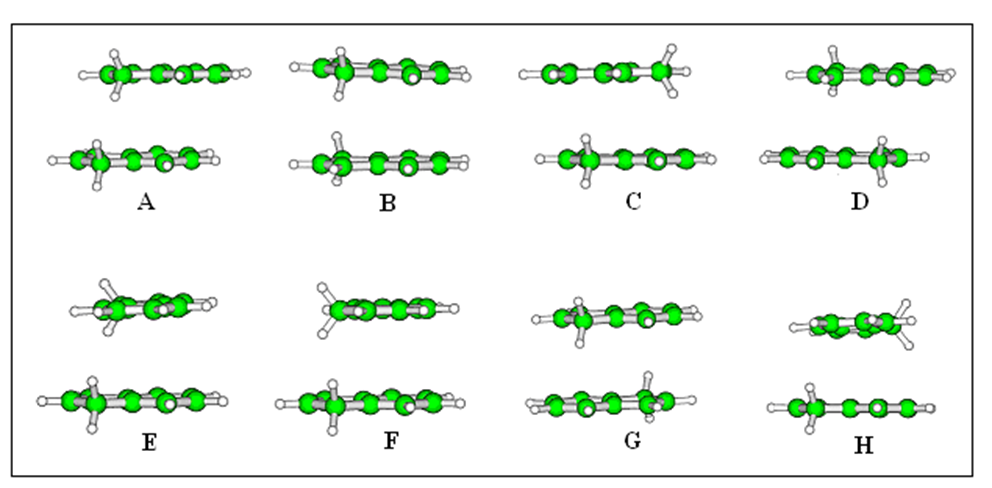
\includegraphics[scale=0.8]{anex/image/Ind-dim}
	\end{center}
	\caption{Configurations of Indene dimers optimized at the $\omega$B97X-D/6-311++G** level of theory.}
\end{figure}



\begin{table}[htbp]
	\caption{Interaction energies of Indene dimers (kcal/mol) in 8 differents configurations using $\omega$B97X-D/6-311++G**, and compared with SAPT-DFT.}
	\begin{tabular}{ccccccccc}
		\toprule
		& \textbf{A} & \textbf{B} & \textbf{C} & \textbf{D} & \textbf{E} & \textbf{F} & \textbf{G} & \textbf{H} \\ 
		\midrule
		\textbf{$\omega$97X-D/
		6-311++G** }& -7.06 & -7.53 & -8.20 & -7.19 & -7.47 & -7.33 & -8.97 & -7.98 \\ 
		\multicolumn{1}{l}{\textbf{SAPT- DFT(PBE0)
				aug-ccpvtz 
			}} & -5.11 & -5.29 & -6.05 & -5.15 & -5.27 & -5.22 & -6.76 & -5.81 \\
			\bottomrule 
		\end{tabular}
		\label{}
	\end{table}
	
	
	

\begin{table}[htbp]
	\caption{Intermolecular distance between ciclopentadiene rings center of  indene dimers (Å). }
	\begin{tabular}{ccccccccc}
		\toprule
		& \textbf{A} & \textbf{B} & \textbf{C} & \textbf{D} & \textbf{E} & \textbf{F} & \textbf{G} & \textbf{H} \\ 
		\midrule
		\textbf{$\omega$97X-D/
			6-311++G** }& 3.98 &3.93 &3.83 &3.67 &4.16 & 3.74 &4.20 &3.96 \\ 
		\multicolumn{1}{l}{\textbf{SAPT- DFT(PBE0)
				aug-ccpvtz 
			}} & 4.01 & 3.96 &3.86 &3.72 &4.21 & 3.78 &4.21 &3.99\\
			\bottomrule 
		\end{tabular}
		\label{}
	\end{table}


\begin{table}[H]
	\caption{Calculated low wavenumber Raman ad PA infrared spectra of Indene Dimer.}
	\begin{center}
			\begin{tabular}{c c c c c c c c}
				\toprule
				\textbf{Mode} & \textbf{$\omega$ cm$^{-1}$} & \multicolumn{1}{p{3cm}}{\centering \textbf{Intensities} \\ \textbf{($^{a}$) [$^{b}$]}} &  &  & \textbf{Mode} & \textbf{$\omega$ cm$^{-1}$} & \multicolumn{1}{p{3cm}}{\centering \textbf{Intensities} \\ \textbf{($^{a}$) [$^{b}$]}}\\
				\midrule	
$\nu_{1}$	&	28	&	(0.04)	[0.00]	&	&	&	$\nu_{7}$	&	205	&	(4.5)	[0.00]\\	
$\nu_{2}$	&	44	&	(0.00)	[8.00]	&	&	&	$\nu_{8}$	&	212	&	(0.00)	[1.15]	\\
$\nu_{3}$	&	62	&	(0.00)	[4.39]	&	&	&	$\nu_{9}$	&	230	&	(0.00)	[0.56]	\\
$\nu_{4}$	&	71	&	(0.34)	[0.00]	&	&	&	$\nu_{10}$	&	238	&	(7.39)	[0.00]	\\
$\nu_{5}$	&	86	&	(0.60)	[0.00]	&	&	&	$\nu_{11}$	&	390	&	(0.00)	[1.09]\\
$\nu_{6}$	&	116	&	(0.00)	[12.40]	&	&	&	$\nu_{12}$	&	390	&(2.78)		[0.00]	\\
\bottomrule
\end{tabular}
\end{center}
\end{table}


		\begin{table}[H]
			\begin{center}
				\begin{threeparttable}
					\begin{tabular}{c c c c c c c c}
						\toprule
						\textbf{Mode} & \textbf{$\omega$ cm$^{-1}$} & \multicolumn{1}{p{3cm}}{\centering \textbf{Intensities} \\ \textbf{($^{a}$) [$^{b}$]}} &  &  & \textbf{Mode} & \textbf{$\omega$ cm$^{-1}$} & \multicolumn{1}{p{3cm}}{\centering \textbf{Intensities} \\ \textbf{($^{a}$) [$^{b}$]}}\\
						\midrule	
$\nu_{13}$	&	400	&(0.00)	[0.95]	&	&	&	$\nu_{18}$	&	547&	(0.00)		[12.10]\\
$\nu_{14}$	&	402&	(9.13) [0.00]	&	&	&	$\nu_{19}$	&	570&	(11.82)	[0.00]\\
$\nu_{15}$	&	432	&(26.07)	[0.00]	&	&	&	$\nu_{20}$	&	570&	(0.00)		[0.50]\\
$\nu_{16}$	&	434	&(0.00)	[0.07]	&	&	&	$\nu_{21}$	&	610&	(2.32)		[0.00]\\
$\nu_{17}$	&	546	&(0.08)	[0.00]	&	&	&	$\nu_{22}$	&	610&	(0.00)		[10.13]\\
					
				\bottomrule
			\end{tabular}
			
			\begin{tablenotes}
				\item[a] km/mole
				\item[b] A$^{4}$/AMU
			\end{tablenotes}
		\end{threeparttable}
	\end{center}
	\label{lowfreq-IndeneDi}
\end{table}	


\begin{table}[H]
	\caption{Calculated Raman and PA infrared spectra of Indene Dimer, 700–2000 cm$^{-1}$}
	\begin{center}
			\begin{tabular}{c c c c c c c c}
				\toprule
				\textbf{Mode} & \textbf{$\omega$ cm$^{-1}$} & \multicolumn{1}{p{3cm}}{\centering \textbf{Intensities} \\ \textbf{($^{a}$) [$^{b}$]}}& &  & \textbf{Mode} & \textbf{$\omega$ cm$^{-1}$} & \multicolumn{1}{p{3cm}}{\centering \textbf{Intensities} \\ \textbf{($^{a}$) [$^{b}$]}}\\
				\midrule	
$\nu_{23}$	&	715	&	0.00)	[0.74]	&	&	&$\nu_{47}$	&	1053	&(0.00)	[47.16]	\\
$\nu_{24}$	&	716	&	(34.29)	[0.00]	&	&	&$\nu_{48}$	&	1053	&(8.74)	[0.00]	\\
$\nu_{25}$	&	742	&	(62.20)	[0.00]	&	&	&$\nu_{49}$	&	1096	&(0.00)	[13.49]	\\
$\nu_{26}$	&	743	&	(0.00)	[0.84]	&	&	&$\nu_{50}$	&	1096	&(3.09)	[0.00]	\\
$\nu_{27}$	&	751	&	(0.00)	[21.71]	&	&	&$\nu_{51}$	&	1140	&(1.96)	[0.00]	\\
$\nu_{28}$	&	752	&	(4.11)	[0.00]	&	&	&$\nu_{52}$	&	1141	&(0.00)	[23.12]	\\
$\nu_{29}$	&	794	&(146.91)	[0.00]	&	&	&$\nu_{53}$	&	1163	&	(4.90)	[0.00]	\\
$\nu_{30}$	&	795	&	(0.00)	[1.79]	&	&	&	$\nu_{54}$	&1164	&	(0.00)	[11.78]	\\
$\nu_{31}$	&	853	&	(0.00)	[17.94]	&	&	&	$\nu_{55}$	&1183	&	(0.16)	[0.00]	\\
$\nu_{32}$	&	853	&	(2.18)	[0.002]	&	&	&	$\nu_{56}$	&1184	&	(0.00)	[5.36]	\\
$\nu_{33}$	&	880	&	(0.00)	[9.36]	&	&	&	$\nu_{57}$	&	1196	&(0.00)	[1.84]\\
$\nu_{34}$	&	880	&	(3.55)	[0.00]	&	&	&	$\nu_{58}$	&1197	&	(2.81)	[0.00]	\\	
$\nu_{35}$	&	884	&	(0.00)	[1.33]	&	&	&$\nu_{59}$	&	1241	&	(0.00)	[45.29]	\\
$\nu_{36}$	&	885	&	(1.51)	[0.00]	&	&	&$\nu_{60}$	&	1242	&	(3.21)	[0.00]	\\
$\nu_{37}$	&	947	&	(16.20)	[0.00]	&	&	&$\nu_{61}$	&	1265	&	(5.49)	[0.00]	\\
$\nu_{38}$	&	947	&	(0.00)	[1.05]	&	&	&$\nu_{62}$	&	1266	&	(0.00)	[24.77]	\\
$\nu_{39}$	&	967	&	(0.00)	[1.24]	&	&	&$\nu_{63}$	&	1327	&	(0.00)	[11.63]	\\
$\nu_{40}$	&	969	&	(2.21)	[0.00]	&	&	&$\nu_{64}$	&	1327	&	(1.37)	[0.00]	\\
$\nu_{41}$	&	971	&	(0.00)	[7.77]	&	&	&$\nu_{65}$	&	1352	&	(0.00)	[11.06]	\\
$\nu_{42}$	&	971	&	(13.75)	[0.00]	&	&	&$\nu_{66}$	&	1353	&	(7.05)	[0.00]	\\
$\nu_{43}$	&	985	&	(3.54)	[0.00]	&	&	&$\nu_{67}$	&	1401	&	(4.87)	[0.00]	\\
$\nu_{44}$	&	986	&	(0.00)	[5.74]	&	&	&$\nu_{68}$	&	1401	&	(0.00)	[42.12]	\\
$\nu_{45}$	&	1007	&	(0.00)	[0.20]	&	&&$\nu_{69}$	&	1439&	(0.01)	[24.51]	\\
$\nu_{46}$	&	1008	&	(0.21)	[0.00]	&	&	&	$\nu_{70}$	&	1439	&	(18.54)	[0.01]	\\
\bottomrule
\end{tabular}
\end{center}
\end{table}


\begin{table}[H]
	\caption{Calculated Raman and PA infrared spectra of Indene Dimer, 700–2000 cm$^{-1}$}
	\begin{center}
		\begin{threeparttable}
			\begin{tabular}{c c c c c c c c}
				\toprule
				\textbf{Mode} & \textbf{$\omega$ cm$^{-1}$} & \multicolumn{1}{p{3cm}}{\centering \textbf{Intensities} \\ \textbf{($^{a}$) [$^{b}$]}}& &  & \textbf{Mode} & \textbf{$\omega$ cm$^{-1}$} & \multicolumn{1}{p{3cm}}{\centering \textbf{Intensities} \\ \textbf{($^{a}$) [$^{b}$]}}\\
				\midrule	
$\nu_{71}$	&	1505	&	(10.12)	[0.00]	&&&	$\nu_{76}$	&	1634	&	(0.00)	[122.78]\\
$\nu_{72}$	&	1505	&	(0.00)	[8.24]	&&&	$\nu_{77}$	&	1667	&	(0.00)	[40.40]\\
$\nu_{73}$	&	1510	&	(0.00)	[21.80]	&&&	$\nu_{78}$	&	1668	&	(0.86)	[0.00]\\
$\nu_{74}$	&	1511	&	(23.19)	[0.00]	&&&	$\nu_{79}$	&	1689	&	(5.18)	[0.00]\\
$\nu_{75}$	&	1634	&	(0.66)	[0.00]	&&&	$\nu_{80}$	&	1689	&	(0.00)	[102.66]\\
			\bottomrule
			\end{tabular}
			
			\begin{tablenotes}
				\item[a] km/mole
				\item[b] A$^{4}$/AMU
			\end{tablenotes}
		\end{threeparttable}
	\end{center}
	\label{freq-IndeneDi}
\end{table}	


\begin{figure}[H]
	\begin{center}
		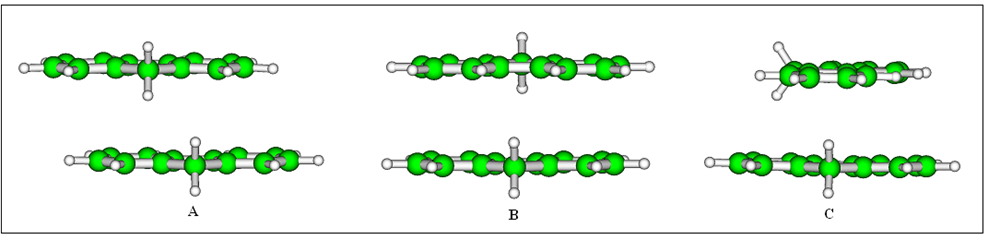
\includegraphics[scale=0.9]{image/Fluo-dim}
	\end{center}
	\caption{ Configurations of Fluorene dimers optimized at the $\omega$B97x-D/6-311++G** level of theory. }
\end{figure}


\begin{table}[htbp]
	\caption{Interaction energies of Fluorene dimers (kcal/mol) in 3 different configurations using $\omega$B97x-D/6-311++G**.}
	\begin{center}
		\begin{tabular}{cccc}
			\toprule
			& \textbf{A} & \textbf{B} & \textbf{C} \\ 
			\midrule
			\textbf{$\omega$B97x-D/
				6-311++G** }& -10.82	& -11.74	& -13.61	\\ 
			\bottomrule
		\end{tabular}
	\end{center}
	\label{}
\end{table}


	\begin{table}[H]
		\caption{Calculated low wavenumber Raman ad PA infrared spectra of Fluorene Dimer.}
		\begin{center}
			\begin{threeparttable}
				\begin{tabular}{c c c c c c c c}
					\toprule
					\textbf{Mode} & \textbf{$\omega$ cm$^{-1}$} & \multicolumn{1}{p{3cm}}{\centering \textbf{Intensities} \\ \textbf{($^{a}$) [$^{b}$]}} &  &  & \textbf{Mode} & \textbf{$\omega$ cm$^{-1}$} & \multicolumn{1}{p{3cm}}{\centering \textbf{Intensities} \\ \textbf{($^{a}$) [$^{b}$]}}\\
					\midrule	
					$\nu_{1}$ & 27 & (0.01) [2.45] &  &  & $\nu_{18}$ & 423 & (0.15)  [10.09] \\ 
					$\nu_{2}$ & 40 & (0.04)  [7.86] &  &  & $\nu_{19}$ & 426 & (8.62)  [2.33] \\ 
					$\nu_{3}$ & 45 & (0.01)  [7.26] &  &  & $\nu_{20}$ & 427 & (0.02)  [2.13] \\ 
					$\nu_{4}$ & 76 & (0.002)  [1.94] &  &  & $\nu_{21}$ & 443 & (0.42) [1.17] \\ 
					$\nu_{5}$ & 79 & (0.05)  [1.55] &  &  & $\nu_{22}$ & 444 & (0.37)  [0.84] \\ 
					$\nu_{6}$ & 93 & (0.02  [3.82] &  &  & $\nu_{23}$ & 484 & (0.001)  [1.08] \\ 
					$\nu_{7}$ & 111 & (0.74)  [0.36] &  &  & $\nu_{24}$ & 486 & (3.56)  [0.10] \\ 
					$\nu_{8}$ & 144 & (0.07)  [0.75] &  &  & $\nu_{25}$ & 502 & (0.21)  [0.05] \\ 
					$\nu_{9}$ & 144 & (0.03)  [1.60] &  &  & $\nu_{26}$ & 503 & (0.32)  [0.35] \\ 
					$\nu_{10}$ & 158 & (0.01)  [0.48] &  &  & $\nu_{27}$ & 558 & (0.16)  [0.75] \\ 
					$\nu_{11}$ & 218 & (0.20)  [0.49] &  &  & $\nu_{28}$ & 558 & (0.27)  [12.06] \\ 
					$\nu_{12}$ & 219 & (0.13  [0.58] &  &  & $\nu_{29}$ & 582 & (0.01)  [0.10] \\ 
					$\nu_{13}$ & 266 & (0.02)  [1.06] &  &  & $\nu_{30}$ & 584 & (0.08)  [0.31] \\ 
					$\nu_{14}$ & 272 & (15.68)  [1.55] &  &  & $\nu_{31}$ & 640 & (3.47)  [0.06] \\ 
					$\nu_{15}$ & 292 & (0.14)  [4.88] &  &  & $\nu_{32}$ & 640 & (5.65)  [0.26] \\ 
					$\nu_{16}$ & 292 & (4.08)  [3.92] &  &  & $\nu_{33}$ & 649 & (0.24)  [0.01] \\ 
					$\nu_{17}$ & 422 & (9.91)  [1.50] &  &  & $\nu_{34}$ & 650 & (0.12)  [0.10] \\ 	
					\bottomrule
				\end{tabular}
				
				\begin{tablenotes}
					\item[a] km/mole
					\item[b] A$^{4}$/AMU
				\end{tablenotes}
			\end{threeparttable}
		\end{center}
		\label{lowfreq-FluoreneDi}
	\end{table}	
	
	
	
	\begin{table}[H]
		\caption{Raman ad PA infrared spectra of Fluorene Dimer, 700- 2000 cm$^{-1}$}
		\begin{center}
				\begin{tabular}{c c c c c c c c}
					\toprule
					\textbf{Mode} & \textbf{$\omega$ cm$^{-1}$} & \multicolumn{1}{p{3cm}}{\centering \textbf{Intensities} \\ \textbf{($^{a}$) [$^{b}$]}} &  &  & \textbf{Mode} & \textbf{$\omega$ cm$^{-1}$} & \multicolumn{1}{p{3cm}}{\centering \textbf{Intensities} \\ \textbf{($^{a}$) [$^{b}$]}}\\
					\midrule
$\nu_{35}$	&	718	&	(0.03)	[0.58]	&	&	&	$\nu_{47}$	&	863	&	(0.10)	[5.61]\\
$\nu_{36}$	&	718	&	(18.08)	[0.06]	&	&	&	$\nu_{48}$	&	863	&	(0.10)	[30.70]\\
$\nu_{37}$	&	747	&	(15.67)	[0.41]	&	&	&	$\nu_{49}$	&	880	&	(2.27)	[0.52]\\
$\nu_{38}$	&	750	&	(1.89)	[0.50]	&	&	&	$\nu_{50}$	&	881	&	(5.50)	[0.30]\\
$\nu_{39}$	&	761	&	(275.51) [0.08]	&	&	&	$\nu_{51}$	&	891	&	(0.26)	[0.002]\\
$\nu_{40}$	&	765	&	(1.77)	[1.61]	&	&	&	$\nu_{53}$	&	943	&	(0.01)	[1.26]\\
$\nu_{41}$	&	765	&	(0.01)	[25.21]	&	&	&	$\nu_{54}$	&	943	&	(0.41)	[0.11]\\
$\nu_{42}$	&	765	&	(0.16)	[13.68]	&	&	&	$\nu_{55}$	&	970	&	(0.26)	[0.02]\\
$\nu_{43}$	&	806	&	(1.33)	[2.69]	&	&	&	$\nu_{56}$	&	971	&	(0.15)	[0.08]\\
$\nu_{44}$	&	807	&	(2.27)	[2.36]	&	&	&	$\nu_{57}$	&	978	&	(13.33)	[0.21]\\
$\nu_{45}$	&	826	&	(0.04)	[0.10]	&	&	&	$\nu_{58}$	&	989	&	(0.01)	[0.98]\\
$\nu_{46}$	&	826	&	(0.02)	[0.35]	&	&	&	$\nu_{59}$	&	1006&	(0.21)	[0.32]\\		
	
	\bottomrule
\end{tabular}
\end{center}
\end{table}






	\begin{table}[H]
		\begin{center}
			\begin{threeparttable}
				\begin{tabular}{c c c c c c c c}
					\toprule
					\textbf{Mode} & \textbf{$\omega$ cm$^{-1}$} & \multicolumn{1}{p{3cm}}{\centering \textbf{Intensities} \\ \textbf{($^{a}$) [$^{b}$]}}& &  & \textbf{Mode} & \textbf{$\omega$ cm$^{-1}$} & \multicolumn{1}{p{3cm}}{\centering \textbf{Intensities} \\ \textbf{($^{a}$) [$^{b}$]}}\\
					\midrule
$\nu_{60}$	&	1008&	(0.48)	[0.24]	&	&	&	$\nu_{37}$	&1331	&	(0.52)	[31.59]\\
$\nu_{61}$	&	1008&	(0.28)	[0.12]	&	&	&	$\nu_{38}$	&1331	&	(0.03)	[117.03]\\
$\nu_{62}$	&	1009&	(0.02)	[0.18]	&	&	&	$\nu_{39}$	&1337	&	(1.89)	[0.05]\\
$\nu_{63}$	&	1034&	(1.63)	[0.91]	&	&	&	$\nu_{40}$	&1337	&(2.26)	[1.26]\\		
$\nu_{64}$	&	1034&	(2.57)	[1.62]	&	&	&	$\nu_{41}$	&1357	&	(7.71)	[1.06]\\
$\nu_{65}$	&	1057&	(0.02)	[94.68]	&	&	&	$\nu_{42}$	&1358	&	(5.36)	[0.002]\\
$\nu_{66}$	&	1058&	(1.58)	[4.53]	&	&	&	$\nu_{43}$	&1381	&	(0.41)	[29.60]\\
$\nu_{67}$	&	1061&	(4.39)	[0.36]	&	&	&	$\nu_{44}$	&1381	&	(0.09)	[51.06]\\
$\nu_{68}$	&	1061&	(7.88)	[2.55]	&	&	&	$\nu_{45}$	&1452	&	(5.88)	[29.20]\\
$\nu_{69}$	&	1128&	(4.32)	[1.05]	&	&	&	$\nu_{46}$	&1452	&	(12.93)	[1.19]\\
$\nu_{70}$	&	1129&	(2.71)	[6.44]	&	&	&	$\nu_{47}$	&1495	&	(7.54)	[1.19]\\
$\nu_{71}$	&	1143&	(0.01)	[0.61]	&	&	&	$\nu_{48}$	&1495	&	(10.03)	[4.70]\\
$\nu_{72}$	&	1143&	(0.02)	[0.03]	&	&	&	$\nu_{49}$	&1498	&	(20.07)	[0.61]\\
$\nu_{73}$	&	1177&	(0.44)	[3.33]	&	&	&	$\nu_{50}$	&1499	&	(25.63)	[1.26]\\
$\nu_{74}$	&	1178&	(0.69)	[4.58]	&	&	&	$\nu_{51}$	&1528	&	(5.12)	[1.65]\\
$\nu_{75}$	&	1182&	(0.20)	[9.65]	&	&	&	$\nu_{52}$	&1529	&	(8.30)	[9.70]\\
$\nu_{76}$	&	1182&	(0.47)	[0.88]	&	&	&	$\nu_{53}$	&1534	&	(0.02)	[66.91]\\
$\nu_{77}$	&	1186&	(0.002)	[16.57]	&	&	&	$\nu_{54}$	&1534	&	(1.26)	[43.91]\\
$\nu_{78}$	&	1186&	(0.10)	[0.03]	&	&	&	$\nu_{55}$	&1652	&	(0.33)	[37.41]\\
$\nu_{79}$	&	1202&	(1.44)	[1.07]	&	&	&	$\nu_{56}$	&1652	&	(0.99)	[14.28]\\
$\nu_{80}$	&	1202&	(0.95)	[0.40]	&	&	&	$\nu_{57}$	&1660	&	(0.98)	[0.80]\\
$\nu_{31}$	&	1223&	(2.59)	[8.74]	&	&	&	$\nu_{58}$	&1660	&	(1.38)	[1.11]\\
$\nu_{32}$	&	1223&	(5.15)	[0.89]	&	&	&	$\nu_{59}$	&1686	&	(1.26)	[11.36]\\
$\nu_{33}$	&	1238&	(2.90)	[1.33]	&	&	&	$\nu_{60}$	&1687	&	(2.21)	[39.23]\\
$\nu_{34}$	&	1238&	(4.86)	[18.36]	&	&	&	$\nu_{61}$	&1692	&	(0.01)	[209.97]\\
$\nu_{35}$	&	1269&(2.36)	[36.28]	&	&	&	$\nu_{62}$	&	1693&	(0.07) [243.77]\\ $\nu_{36}$	&	1270	&	(0.57)	[108.92]	&	&	&	&  &  \\				
					
					\bottomrule
				\end{tabular}
				
				\begin{tablenotes}
					\item[a] km/mole
					\item[b] A$^{4}$/AMU
				\end{tablenotes}
			\end{threeparttable}
		\end{center}
		\label{freq-FluoreneDi}
	\end{table}					


\begin{figure}[H]
	\begin{center}
		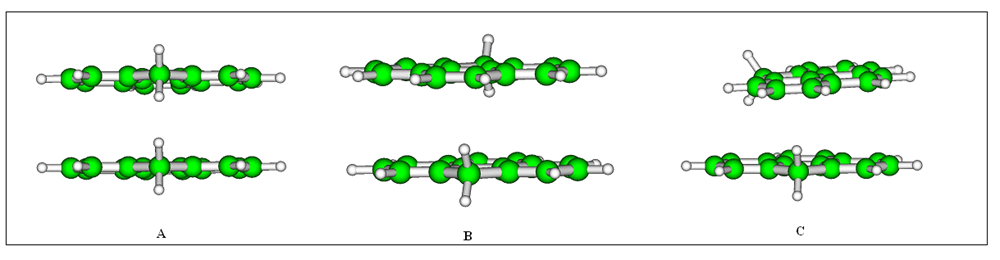
\includegraphics[scale=0.9]{anex/image/TCC}
	\end{center}
	\caption{ Configurations of Cyclopentaphenanthrene dimers optimized at the $\omega$B97x-D/6-311++G** level of theory. }
\end{figure}

\begin{table}[htbp]
	\caption{Interaction energies of Cyclopentaphenanthrene dimers (kcal/mol) in 3 different configurations using $\omega$B97x-D/6-311++G**.}
	\begin{center}
		\begin{tabular}{cccc}
			\toprule
			& \textbf{A} & \textbf{B} & \textbf{C} \\ 
			\midrule
			\textbf{$\omega$B97x-D/
				6-311++G** }& -13.20	& -14.61	& -15.21	\\ 
			\bottomrule
		\end{tabular}
	\end{center}
	\label{}
\end{table}

	\begin{table}[H]
		\caption{Calculated low wavenumber Raman ad PA infrared spectra of Cyclopentaphenanthrene Dimer.}
		\begin{center}
			\begin{threeparttable}
				\begin{tabular}{c c c c c c c c}
					\toprule
					\textbf{Mode} & \textbf{$\omega$ cm$^{-1}$} & \multicolumn{1}{p{3cm}}{\centering \textbf{Intensities} \\ \textbf{($^{a}$) [$^{b}$]}} &  &  & \textbf{Mode} & \textbf{$\omega$ cm$^{-1}$} & \multicolumn{1}{p{3cm}}{\centering \textbf{Intensities} \\ \textbf{($^{a}$) [$^{b}$]}}\\
					\midrule	
$\nu_{1}$ & 29 & (0.00) [1.77] & & & $\nu_{21}$& 447& (0.02) [16.59]\\
$\nu_{2}$ & 34 & (0.07) [10.73] & & & $\nu_{22}$& 447& (0.03) [18.27] \\
$\nu_{3}$ & 45 &  (0.00) [11.47] &  & & $\nu_{23}$& 478& (0.04) [0.66]\\
$\nu_{4}$ & 77& (0.01) [0.48] &  & &  $\nu_{24}$& 478 & (1.20) [0.15]\\
$\nu_{5}$ & 88 & (0.00) [2.91] &  & & $\nu_{25}$&495 & (0.88) [0.51] \\
$\nu_{6}$ &  90 & (0.32) [0.13] & & & $\nu_{26}$& 495 & (1.02) [3.95] \\
$\nu_{7}$ & 110 & (4.19) [0.90] & & & $\nu_{27}$&508 & (6.63) [0.01] \\
$\nu_{8}$ & 116 & (0.02) [0.92] & & & $\nu_{28}$&510 & (0.24) [0.36] \\
$\nu_{9}$ & 194 & (0.08) [1.62] & & & $\nu_{29}$& 534 & (0.28) [0.14]\\
$\nu_{10}$ & 195 & (0.01) [0.95] & & & $\nu_{30}$&534 & (0.77) [0.41]\\
$\nu_{11}$ & 206 & (25.22) [0.75] & & & $\nu_{31}$& 560 & (0.01) [0.44]\\
$\nu_{12}$ & 210 & (0.00) [3.23] & & & $\nu_{32}$& 561 & (0.01) [3.40]\\
$\nu_{13}$ & 257& (4.41) [0.57] & & & $\nu_{33}$& 579 & (0.02) [0.03]\\
$\nu_{14}$ & 264 & (0.00) [1.78] & & & $\nu_{34}$&579 & (0.03) [0.11]\\
$\nu_{15}$ & 294 & (0.34) [1.66] & & & $\nu_{35}$& 604& (2.33) [0.09]\\
$\nu_{16}$ & 295 & (0.18) [1.36] & & & $\nu_{36}$&605 & (0.80) [32.26]\\
$\nu_{17}$ & 344& (1.74) [0.50] & & & $\nu_{37}$&632 & (0.02) [0.05] \\
$\nu_{18}$ & 344& (0.82) [0.11] & & & $\nu_{38}$& 635 & (0.10) [0.03]\\
$\nu_{19}$ & 437 & (0.04) [3.63] & & & $\nu_{39}$&672 & (0.47) [0.97] \\
$\nu_{20}$ & 438 & (0.12) [3.09] & & & $\nu_{40}$&672 & (0.28) [40.10]\\
 	\bottomrule
\end{tabular}

\begin{tablenotes}
	\item[a] km/mole
	\item[b] A$^{4}$/AMU
\end{tablenotes}
\end{threeparttable}
\end{center}
\label{lowfreq-CyclopentaDi}
\end{table}	





\begin{figure}[H]
	\begin{center}
		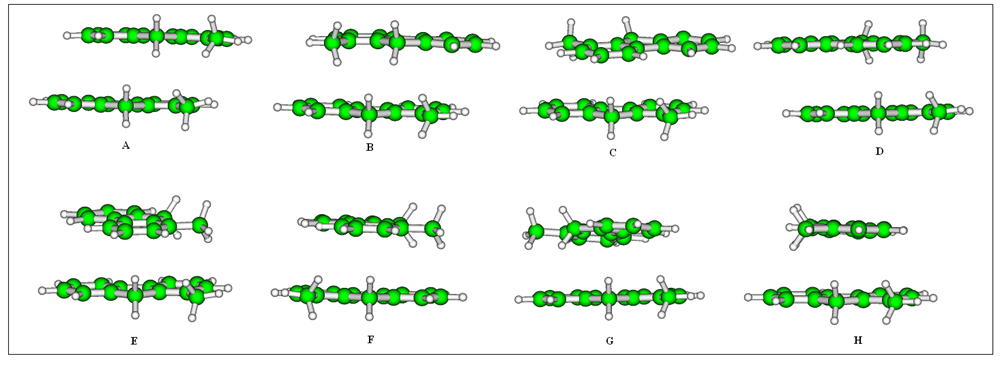
\includegraphics[scale=0.9]{image/1MCC}
	\end{center}
	\caption{ Configurations of 1-methylfluorene dimers optimized at the $\omega$B97x-D/6-311++G** level of theory. }
\end{figure}


\begin{table}[htbp]
	\caption{Interaction energies of 1-methylfluorene dimers (kcal/mol) in 8 differents configurations using $\omega$B97X-D/6-311++G**.}
	\begin{tabular}{ccccccccc}
		\toprule
		&\textbf{A} & \textbf{B} & \textbf{C} & \textbf{D} & \textbf{E} & \textbf{F} & \textbf{G} & \textbf{H} \\ 
		\midrule
		\textbf{$\omega$B97X-D/
		6-311++G**} & -12.13 & -12.92 & -15.78 & -14.95 & -15.94 & -15.45 & -14.80 & -15.01 \\ 
	\bottomrule
	\end{tabular}
	\label{}
\end{table}

\begin{table}[H]
	\caption{Calculated low wavenumber Raman ad PA infrared spectra of 1-methylfluorene Dimer.}
	\begin{center}
		\begin{threeparttable}
			\begin{tabular}{c c c c c c c c}
				\toprule
				\textbf{Mode} & \textbf{$\omega$ cm$^{-1}$} & \multicolumn{1}{p{3cm}}{\centering \textbf{Intensities} \\ \textbf{($^{a}$) [$^{b}$]}} &  &  & \textbf{Mode} & \textbf{$\omega$ cm$^{-1}$} & \multicolumn{1}{p{3cm}}{\centering \textbf{Intensities} \\ \textbf{($^{a}$) [$^{b}$]}}\\
				\midrule	
$\nu_{1}$&  22 & (0.02)  [1.74] &  &    & $\nu_{21}$ & 305 & (0.02)  [4.24]  \\ 
$\nu_{2}$&  40 & (0.00)  [5.00] &  &    & $\nu_{22}$ & 307 & (0.06)  [0.87] \\ 
$\nu_{3}$&  50 & (0.00)  [5.37] &  &    & $\nu_{23}$ & 433 & (1.65)  [0.48] \\ 
$\nu_{4}$&  52 & (0.02)  [3.48] &  &    & $\nu_{24}$ & 435 & (6.42)  [0.21] \\ 
$\nu_{5}$&  69 & (0.06)  [1.53] &  &    & $\nu_{25}$ & 439 & (0.66) [2.04] \\ 
$\nu_{6}$&  87 & (0.71)  [1.80] &  &    & $\nu_{26}$ & 440 & (0.18)  [5.68] \\ 
$\nu_{7}$&  93 & (0.02)  [0.73] &  &    & $\nu_{27}$ & 482 & (3.08)  [0.39] \\ 
$\nu_{8}$&  114 & (1.56)  [0.55] &  &    & $\nu_{28}$&  486 & (0.27)  [0.34] \\ 
$\nu_{9}$&  128 & (0.03)  [3.80] &  &    & $\nu_{29}$ & 508 & (0.04)  [6.34] \\ 
$\nu_{10}$& 131 & (0.12)  [1.77] &  &    & $\nu_{30}$ & 508 & (0.12)  [4.90] \\ 
$\nu_{11}$&  138 & (0.05)  [0.45] &  &    & $\nu_{31}$ & 518 & (1.16)  [0.46] \\ 
$\nu_{12}$&  187 & (0.25)  [0.31] &  &    & $\nu_{32}$ & 522 & (0.48)  [0.76] \\ 
$\nu_{13}$&  189 & (0.07)  [0.45] &  &    & $\nu_{33}$ & 550 & (1.49)  [1.74] \\ 
$\nu_{14}$&  213 & (0.09)  [1.67] &  &    & $\nu_{34}$ & 551 & (0.99)  [2.09] \\ 
$\nu_{15}$&  225 & (0.06)  [0.87] &  &    & $\nu_{35}$ & 589 & (2.08)  [3.48] \\ 
$\nu_{16}$&  245 & (0.06)  [0.61] &  &    & $\nu_{36}$ & 590 & (1.30)  [4.81] \\ 
$\nu_{17}$&  260 & (6.30)  [1.37] &  &    & $\nu_{37}$ & 593 & (2.94)  [0.49] \\ 
$\nu_{18}$&  277 & (14.65)  [1.88] &  &   & $\nu_{38}$ & 598 & (1.25)  [0.61] \\ 
$\nu_{19}$&  285 & (0.21)  [5.54] &  &    & $\nu_{39}$ & 644 & (1.57)  [1.08] \\ 
$\nu_{20}$&  290 & (7.49)  [2.74] &  &    & $\nu_{40}$ & 645 & (3.51  [0.13] \\ 
	\bottomrule
\end{tabular}

\begin{tablenotes}
	\item[a] km/mole
	\item[b] A$^{4}$/AMU
\end{tablenotes}
\end{threeparttable}
\end{center}
\label{lowfreq-1-methylflDi}
\end{table}	





\begin{figure}[H]
	\begin{center}
	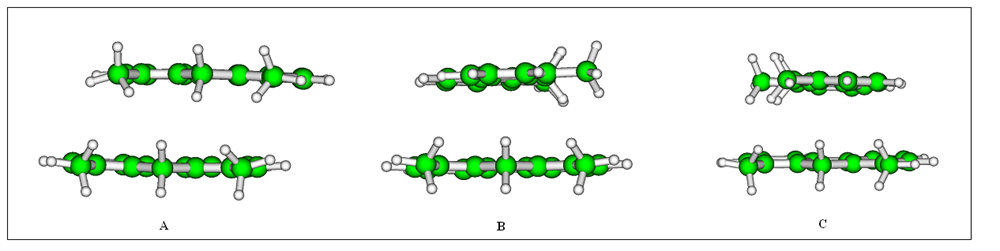
\includegraphics[scale=0.9]{image/18MCC}	
	\end{center}
	\caption{ Configurations of 1,8-dimethylfluorene dimers optimized at the $\omega$B97x-D/6-311++G** level of theory. }
\end{figure}


\begin{table}[htbp]
	\caption{Interaction energies of 18-dimethylfluorene dimers (kcal/mol) in 3 different configurations using $\omega$B97x-D/6-311++G**.}
	\begin{center}
		\begin{tabular}{cccc}
			\toprule
			& \textbf{A} & \textbf{B} & \textbf{C} \\ 
			\midrule
			\textbf{$\omega$B97x-D/
				6-311++G** }& -14.12	& -15.90	& -16.29	\\ 
			\bottomrule
		\end{tabular}
	\end{center}
	\label{}
\end{table}
		
	
		
		
		
		
		
		
		
	
	
